\section{Antinuclei in the cosmos}\label{sec:AntinucleiInTheCosmos}
Antinuclei are some of the rarest stable objects in cosmic rays, in fact, no compound antinuclei have ever been conclusively observed in cosmic rays. But it is this exact fact that makes them such promising candidates for the search of new physics beyond the Standard Model. Whereas for other particle species the signal-to-background ratio might be minuscule for any new effect, antinuclei production is so rare in standard model processes that any new physics might produce signals orders of magnitude greater than what can be explained with our current knowledge. While no conclusive observation of antinuclei in cosmic rays has been published, the AMS-02 Collaboration has repeatedly reported potential signals of antihelium\cite{}, motivating a renewed push of research interest into cosmic-ray antinuclei. \\
%todo: add a small section on primordial black holes (for antideuterons only)
The goal of this section is to discuss possible exotic sources of antinuclei in our galaxy focusing on WIMP dark matter and extragalactic WIMP dark matter. For antideuterons primordial black holes are also discussed as a possible source. These are compared to antinuclei produced in high-energy cosmic-ray collisions with the interstellar medium, which in the respective rest frame is an analogous process to the one used to produce antinuclei at accelerators. In the lab frame the collision is heavily boosted, which affects the produced spectra. Crucially, the new measurements of the inelastic cross sections of antihelium laid out in Section \ref{sec:ResHe3SigmaInel}, and the first low-energy measurements of the antideuteron--matter inelastic cross section laid out in \cite{antideuteronXS}, are for the first time incorporated in such studies. The discussion therefore focuses in particular on propagating these measurements to obtain the experimental uncertainites from inelastic interactions on the antinuclei flux near earth. This journey from creation to observation for antinuclei is illustrated in figure \ref{fig:Galaxy_story}.\\

\begin{figure}[bhtp]
    \centering
    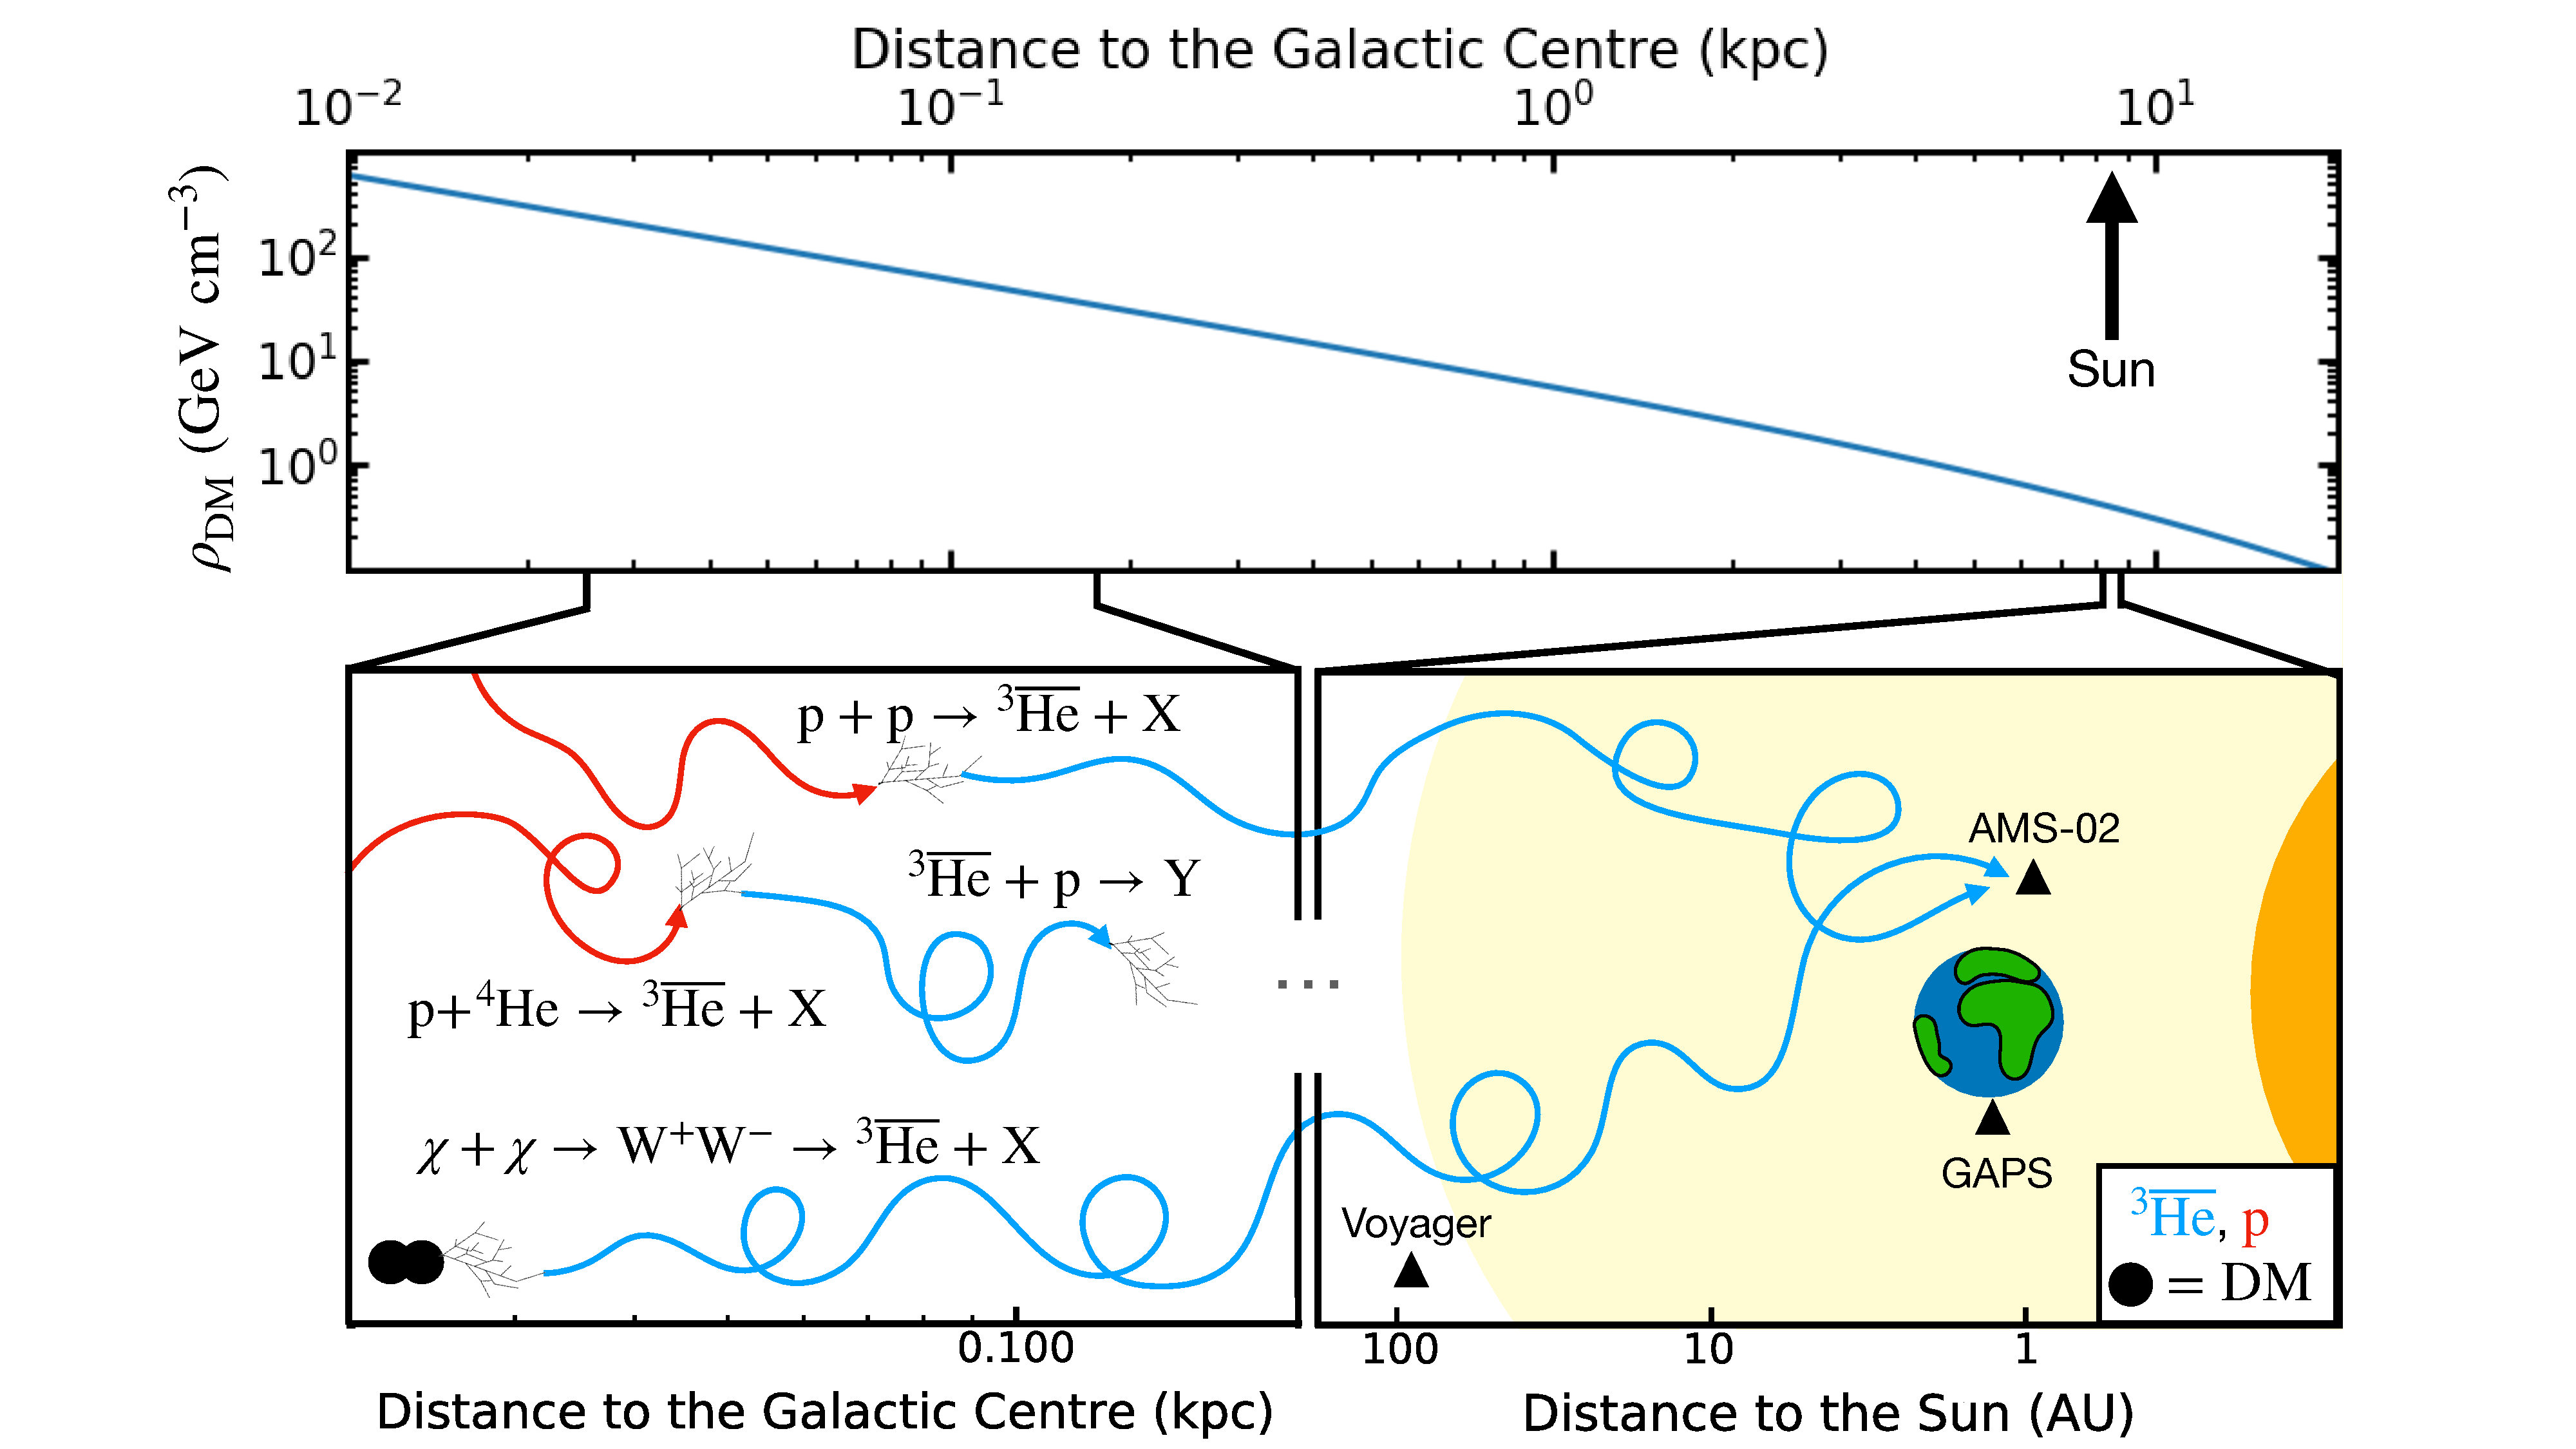
\includegraphics[width=\textwidth]{figures/GalaxyStory.pdf}
    \caption{Illustrated story of the journey which antinuclei undertake before being observed near earth. Red lines shown high energy cosmic ray protons, Blue lines shown \ahe\ . The antinuclei get created all throughout the galaxy, and in the galactic centre antinuclei from dark matter is the most concentrated, due to the higher dark matter density. Similarly, antinuclei from high energy cosmic rays are created all over the galaxy. The created antinuclei then travel through the interstellar medium, some of them annihilating along the way. The ones which do make it to earth then are affected by the solar magnetic field, before reaching detectors near earth. All these processes need to be understood in order to be able to interpret an antinuclei signal in cosmic rays.}
    \label{fig:Galaxy_story}
\end{figure}

In order to study the two sources we employ the GALPROP framework\cite{}. This framework propagates particles through our galaxy, simulating various effects such as diffusion, convection and also inelastic processes. The resulting fluxes near earth are then presented for both antideuterons and \ahe, for different dark matter masses and profiles. Finally, current and planned experiments for detecting antinuclei in cosmic rays are discussed. 
The antinuclei fluxes from high-energy cosmic-ray collisions shown in this thesis as comparisons to the fluxes from possible dark-matter sources are taken from \cite{dbar_prop} and \cite{ALICE-PUBLIC-2022-001}, for antideuteron and \ahe\ respectively.\\




\subsection{Sources of antinuclei in the cosmos}
Antinuclei are some of the rarest stable particles in our galaxy, since very few abundantly occurring processes will produce them in any detectable amount\cite{}. This is in contrast to nuclei, which are the most abundant stable particles within our galaxy. Indeed, nuclei up to Iron have been observed by a variety of methods: in the spectral lines of starts \cite{}, in cosmic rays by the AMS collaboration \cite{} and of course on earth. A large amount of the light matter nuclei (up to Lithium) was produced during Big Bang Nucleosynthesis (BBN)\cite{}, while all heavier nuclei were produced during stellar nucleosynthesis\cite{}. This process involves fusing hydrogen nuclei to create the necessary energy inside a star to counteract its own gravitational pull, creating helium in the process. This continues for most of the lifetime of the star, until its reserves of hydrogen run low. Without the sustained temperature and pressure provided by hydrogen fusion, the star's core will become inert and contract under gravity. Meanwhile, fusion will start in the outer layers of the star, where residual hydrogen is still found. This causes those layers to expand and cool, and the star /forms what is called a red giant\cite{} or red supergiant\cite{}. Over time, the core will contract and heat up\footnote{Red supergiants may have sufficient pressure immedeately to commence helium fusion in their core. For more information on stellar information please refer to \cite{}.}, until the conditions allow for even heavier elements (helium and sometimes carbon) to start fusing to create energy \cite{}. During this process, elements up to iron are created through nuclear fusion, and heavier elements can be created through slow neutron capture processes \cite{}. This process accounts for the production of roughly half of the elements heavier than iron \cite{}. When this source of energy becomes insufficient, the red giant's will implode and expell its outer shell, creating a planetary nebula. Red supergiants will explode in a supernovae\cite{}, expelling huge amounts of energy and matter. In this process, rapid neutron capture occurs, producing the other half of elements heavier than iron\cite{}. \\
However, due to the asymmetry of matter and antimatter in our galaxy, neither BBN nor stellar nucleosynthesis is thought to be a dominant source for antinuclei. Antimatter produced during BBN is likely to have annihilated propagating through the galaxy from the Big Bang until today. This can be shown by a back of the envelop calculation. Assuming an antinucleus with an annihilation cross section of $\approx$1b and a momentum of $\gtrapprox$ 0.1 GeV/n, the fraction surviving until this day is given by $N/N_0 = \mathrm{exp}(-\sigma n \beta c t)$, where $n$ is the average matter density in the regions traversed. Taking $n = 1 \mathrm{cm}^{-3}$ and using $\beta = p/\gamma m$ one finds that only about $e^{-100} \approx 10^{-44}$ of the initial population would still be left today.  And in order for stellar antinucleosynthesis to occur, anti-starts -- or at least large clouds of antimatter -- would have to exists. Any such regions would by default have to come in come in contact with the matter dominated regions which predominantly make up our galaxy. In those overlap regions, significant amounts of annihilations would cause a visible gamma ray signal \cite{}.  No signal of this kind has been reported, although if such regions were small enough, they would appear as point sources to current instruments and thus make up a part of the currently unidentified point sources within our galaxy \cite{Fermi Lat point source catalogue}. Recent work has claimed that such antimatter regions may have formed during the big bang and survived to this day\cite{}, making up $\approx$ 20 of the roughly 1000 unidentified point sources. However, these studies also note the necessity for the antimatter regions to have formed in places where the proton density is O($10^{-8}$) of the cosmic average.  The authors do not provide a viable mechanism by which this could have occurred. \\
We therefore have to look to other processes which could produce antinuclei. Due to baryon number conservation, all such processes are likely to produce at least an equal amount of light nuclei as well. However, since nuclei are far more abundant than antinuclei, these processes will only contribute a negligible amount to the total nuclei flux in our galaxy, while they might dominate the antinuclei flux. This extremely high expected signal-to-background ratio is the reason why antinuclei are considered such a promising probe into new physics.

\subsubsection{High-energy cosmic-ray collisions}
The most well-known source for antinuclei in cosmic rays --- and the only one which does not require new physics or as of yet undiscovered objects --- are collisions of high-energy cosmic rays with the interstellar medium. Such collisions, akin to collisions at particle accelerators, will produce antinuclei by converting the available mass--energy from the collision into (anti)nucleons which then coalesce (see section \ref{sec:IntroProductionAntinuclei} for a more detailed discussion on antinuclei production).  In order to predict the production of antinuclei in such high energy collisions we need to know the differential production cross section of the antinuclei in question, for each collision which can occur, and we need to know which collisions those are, i.e. we need to know the composition of cosmic rays and of the interstellar medium, as a function of energy. For both the interstellar gas and cosmic rays, the composition is $\approx$90\% protons, $\approx$9\% Helium-4 and $<$1\% heavier nuclei. Thus, the source term for nuclei from such secondary collisions can be written as 

\begin{equation}\label{eq:secSourceTerm}
    q (\vec{r}, p) = \sum_{CR=\mathrm{H}, \mathrm{He}} \sum_{ISM=\mathrm{H},\mathrm{He}} n_{ISM}(\vec{r} \int dp_{\mathrm{CR}}' \beta_{\mathrm{CR}} c \frac{d\sigma(p, p_{\mathrm{CR}}')}{dp} n_{\mathrm{CR}}(\vec{r}, p_{\mathrm{CR}}')
\end{equation}

, where $\sum_{CR=\mathrm{H}, \mathrm{He}} \sum_{ISM=\mathrm{H},\mathrm{He}}$ denote the sums over the particle species in cosmic rays and the interstellar medium, $n_{ISM}(\vec{r})$ is the density of the interstellar gas at a given point, $n_{\mathrm{CR}}(\vec{r}, p_{\mathrm{CR}}')$ is the density of cosmic rays at a given position and energy, and $\frac{d\sigma(p, p_{\mathrm{CR}}')}{dp}$ is the differential production cross section for an antinucleus, as a function of the momentum of the produced antinucleus $p$ and the momentum of the incoming cosmic ray $p_{\mathrm{CR}}'$. The particles in the interstellar medium are considered to be at rest in this calculation, which is a valid approximation since they move at  very low speeds in comparison to the incoming cosmic rays\footnote{Interstellar gas particles can be expected to move at speeds of the order of the rotational velocity of the milky way, which is O(100 km/s) or O($\beta = 10^-4$). This is much lower than the velocity of incoming protons at the threshold for antinuclei production, where O($\beta >0.999$).}. \\

The production cross section of antinuclei in such small collisions systems is suppressed at low energies due to the baryon number conservation, since it is necessary to produce at least 4 (6) new nucleons in order to produce antideuterons (\ahe). The requirement for these additional nucleons means that the threshold of the required COM energy is about $\sqrt{s}_{\mathrm{th}}\approx 6 (8)  m_p$ for antideuterons (\ahe ). Given that the ISM target is at rest, all the energy must come from the incoming cosmic ray particle. This means that the frame of reference of the collision will be highly boosted in comparison to the galactic frame, and that the centre of mass energy will only rise $\propto \sqrt{E_\mathrm{CR}}$. 
In the case of \ahe\ this corresponds to a threshold energy of the incoming proton of $E_p \approx 31$ GeV. In order to estimate these cross sections, Monte Carlo event generators are used to create the proton and neutron spectra and distributions, and coalescence afterburners are then applied in order to estimate the production of antinuclei. In this work, the production cross sections by \cite{Shukla} and \cite{Gomez} are used, referred to hereinafter as Shukla et. al. For \ahe\, O($10^{11}-10^{12}$) events are needed to get a statistical precision on the \% level on the total yield for a given incoming beam energy\cite{Shukla}. The resulting production cross sections for \ahe\ and antideuterons are shown in figure \ref{fig:CR_production_XS}, where they are shown for a wide array of incoming beam energies. As can be seen, it requires significantly above the threshold energy of $\sqrt{s}=$31 GeV in ordet to produce any significant \ahe\ flux\footnote{It is the lowest energy considered for antideuterons since the same simulations were used to determine both sets of spectra in Shukla et. al.}.

\begin{figure}[htbp]
    \centering
    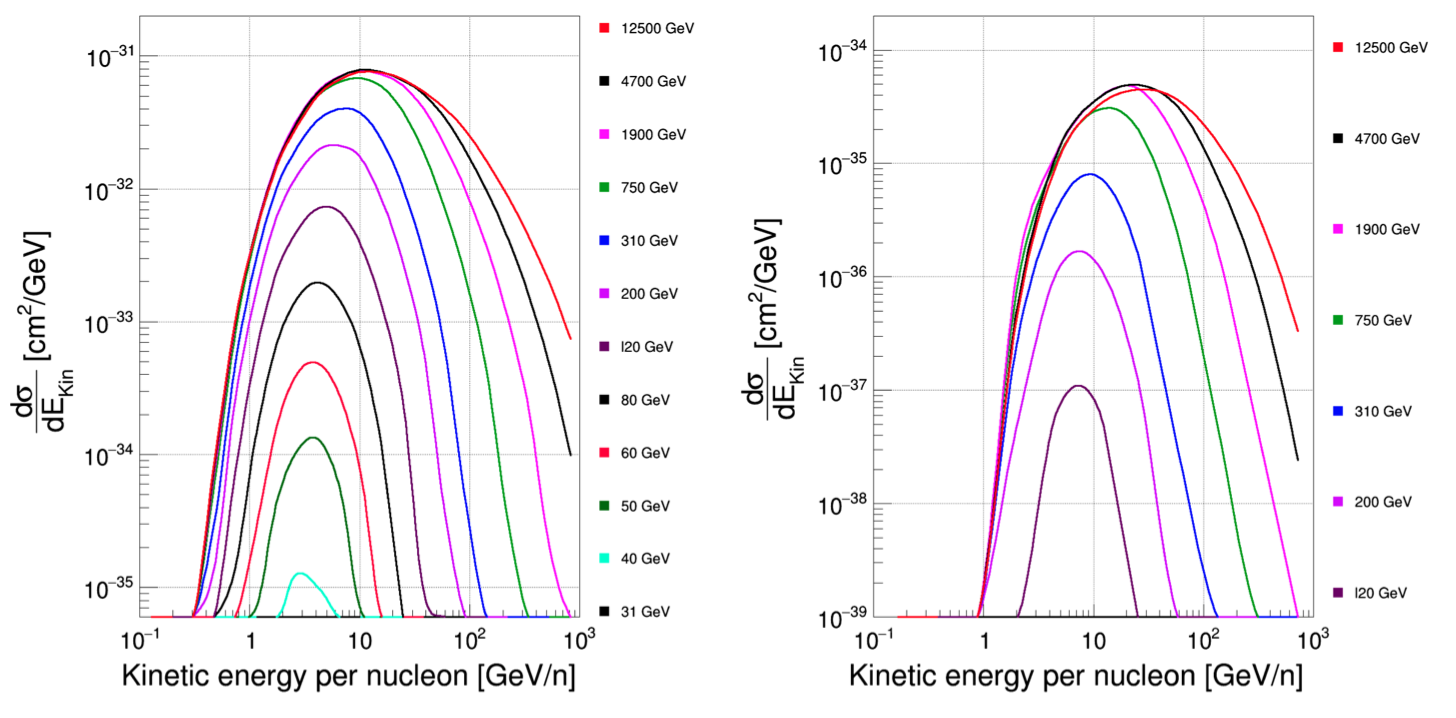
\includegraphics[width=\textwidth]{figures/production_xs_shukla.png}
    \caption{Production cross section for antideuterons (left) and \ahe\ (right), as a function of the energy of the antinucleus produced, for a range of different projectile energies, taken from Shukla et. al. The \ahe\ cross section includes the effect of antitritons which are produced and subsequently decay to \ahe\ . }
    \label{fig:CR_production_XS}
\end{figure}

The cross sections shown are constrained by data from a variety of accelerator experiments. The list of experiments used to constrain the production cross for antideuterons is shown in figure \ref{fig:dbar_prod_v_rapidity}, while for \ahe\ the data is very scarce for p-p collisions at low energies. In order to validate the production, the authors instead used their model to simulate pp collisions at $\sqrt{s}=7$ TeV, in order to compare with ALICE data. The resulting fit is shown in figure \ref{fig:prod_v_ALICE}, where the uncertainties are obtained by varying the coalescence momentum by 30\%. It can be seen from figure \ref{fig:dbar_prod_v_rapidity}, for $\sqrt{s} \gtrapprox 25$ GeV, there are only measurements at mid-rapidity. However, due to the highly boosted nature of the frame in CR collisions, antinuclei are likely to be produced at very forward rapidities. Thus, further experimental searches at forward rapidity are needed in order to better constrain antinuclei production in high energy CR collisions.  

\begin{figure}[htbp]
    \centering
    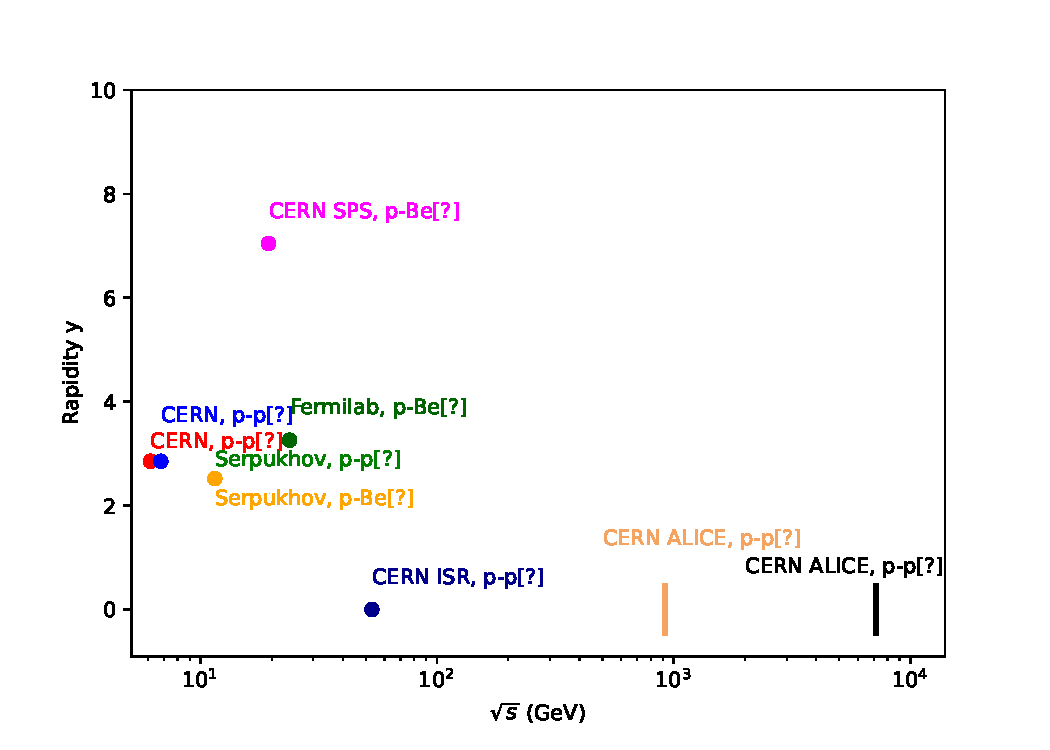
\includegraphics[width=\textwidth]{figures/dbar_production_experiments_sqrts_v_rapidity.pdf}
    \caption{A list of experiments with measurements of (anti)deuteron production, as a function of rapidity and $\sqrt{s}$. The compilation is taken from table 2 in \cite{Gomez}.}
    \label{fig:dbar_prod_v_rapidity}
\end{figure}

\begin{figure}[htbp]
    \centering
    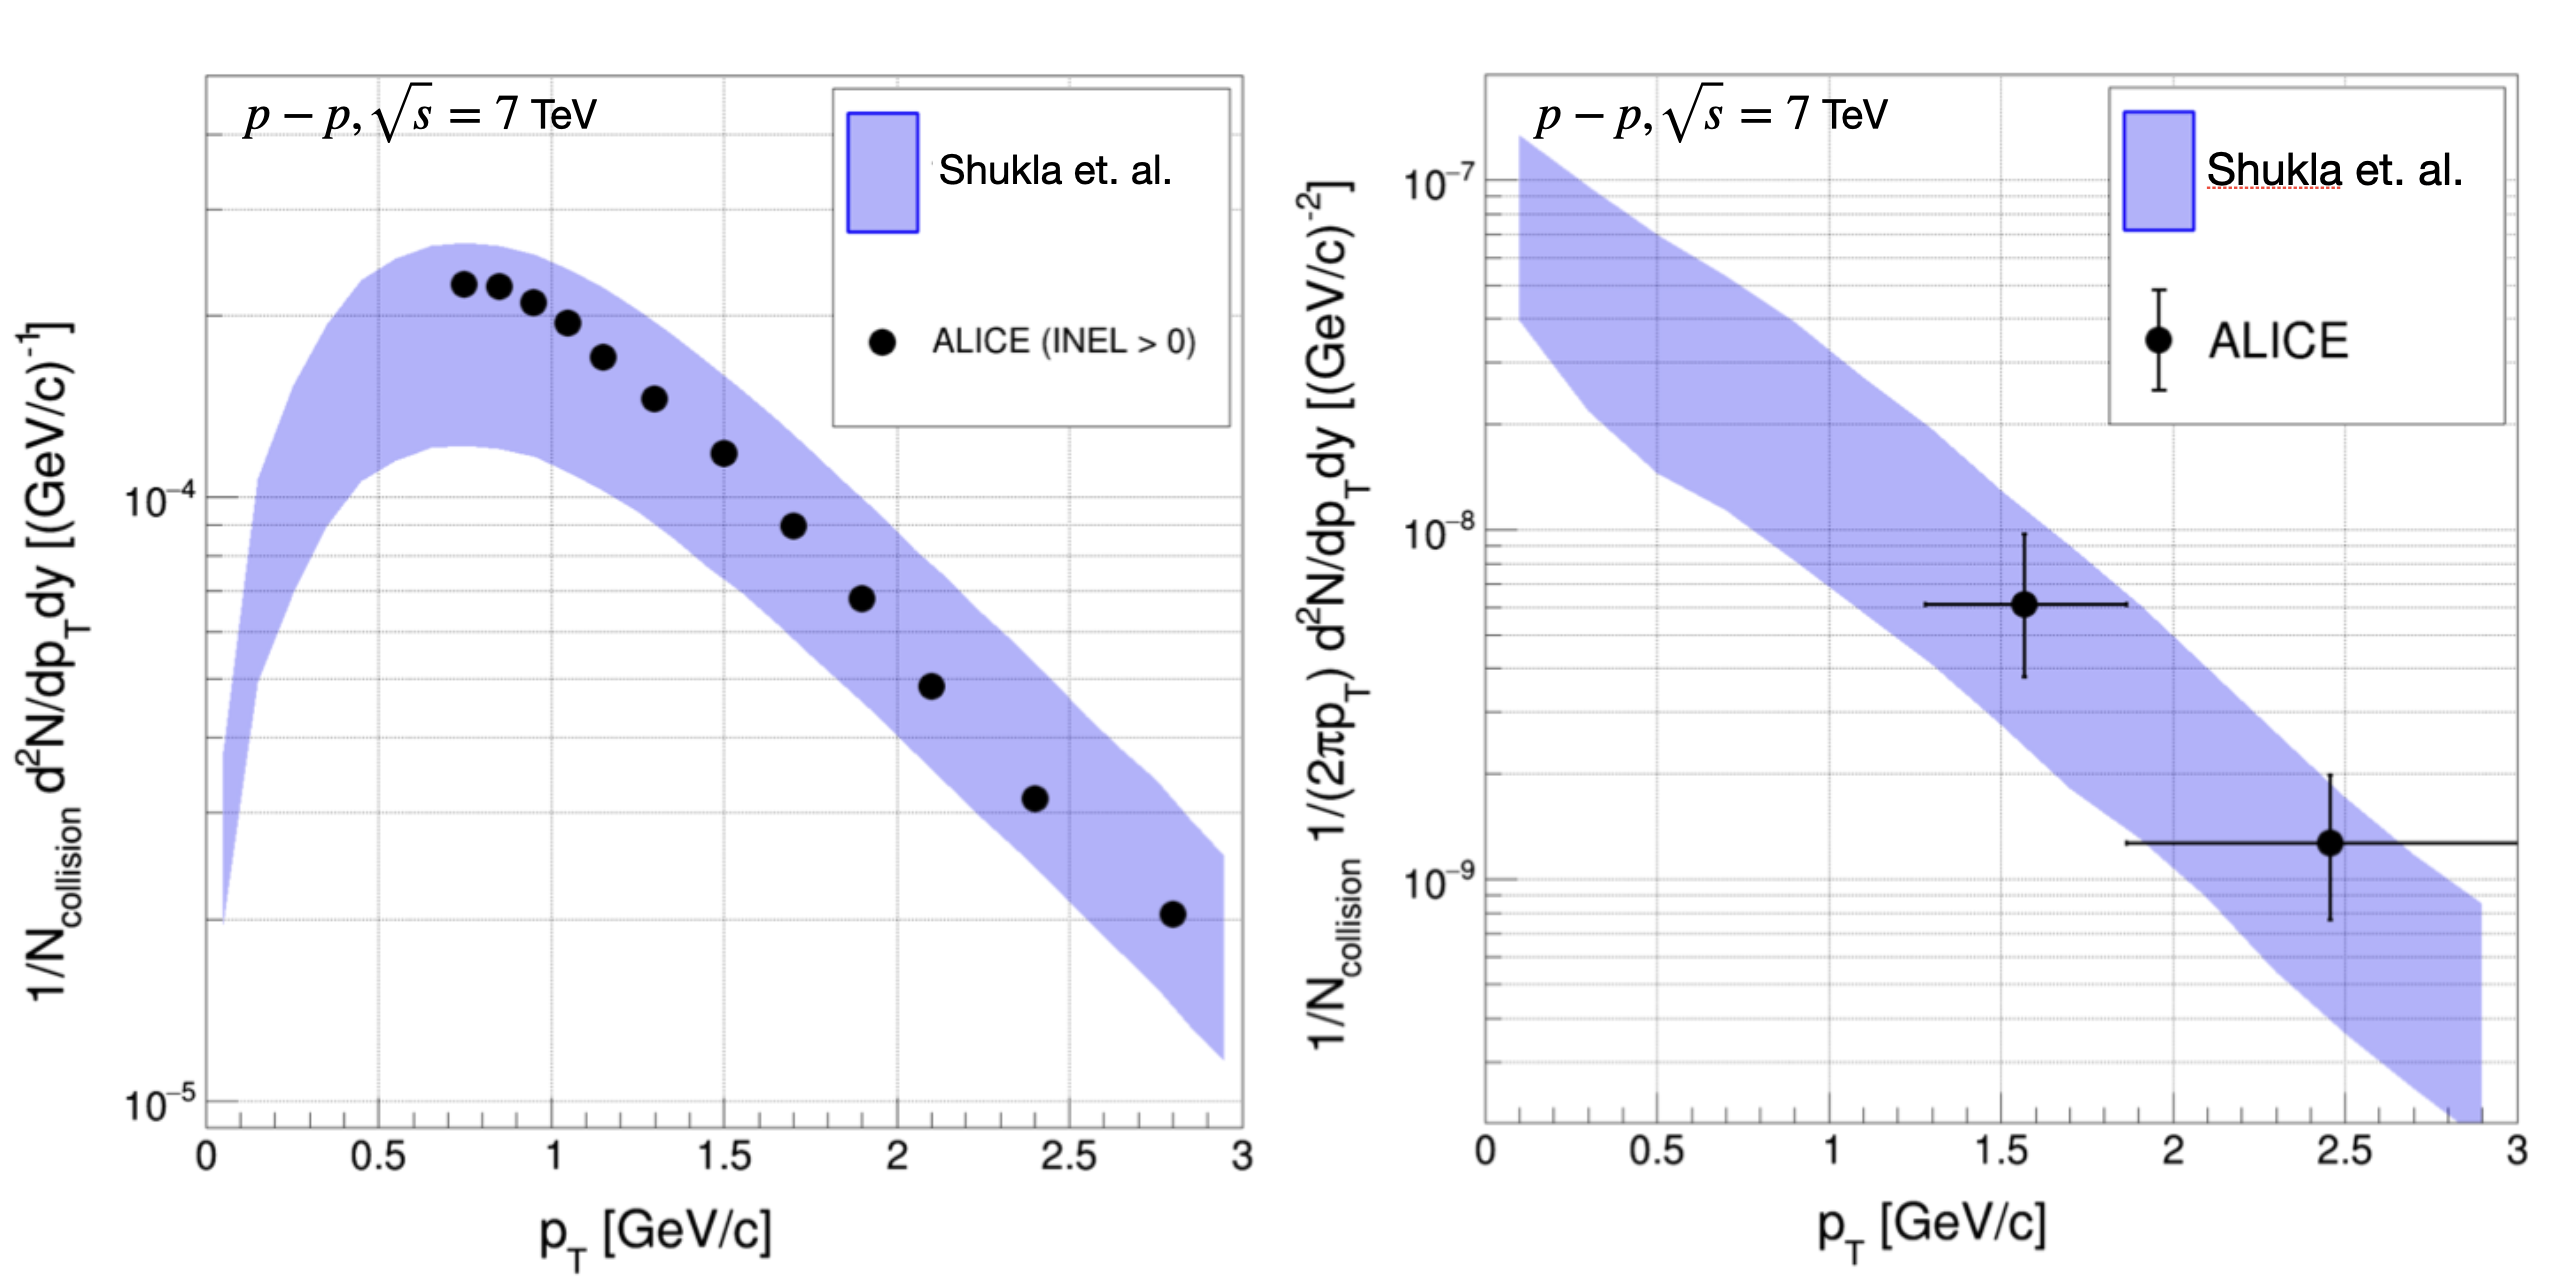
\includegraphics[width=\textwidth]{figures/production_xs_ALICE_comparison.png}
    \caption{Comparison of the antideuteron (left) and \ahe\ (right) spectra obtained by Shukla et. al. with ALICE data for $\sqrt{s}=7$ TeV pp collisions.}
    \label{fig:prod_v_ALICE}
\end{figure}

Once these cross sections are obtained, they need to be folded with the galactic cosmic ray spectrum at each point in space. This spectrum spans over more than 11 orders of magnitude if all particles are considered, and at least 6 orders of magnitude for protons. A compilation of available data on the cosmic ray spectrum can be found in figure \ref{fig:CR_spectra_Thomas}. The implementation of this process in Galprop is done by implementing the cross section above, and thus calculating equation \ref{eq:secSourceTerm} at each point in the space/momentum grid employed in GALPROP. For a more detailed discussion of Galprop see section \ref{sec:GALPROP}. Also shown in the left of this figure is the source term of antideuterons, as a function of both the incoming particle momentum and the momentum of the produced antideuteron. From this it can be seen that the most important momentum range to probe is 100-500 GeV/$c$. 

\begin{figure}
    \centering
    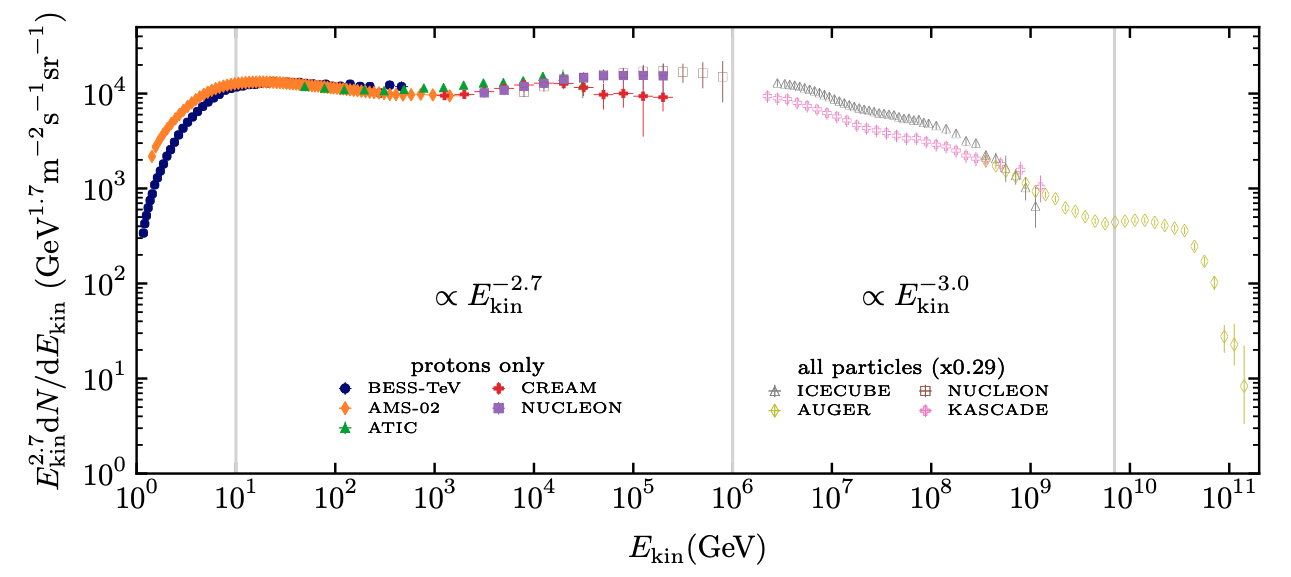
\includegraphics[width=0.62\textwidth]{figures/ThomasP_cosmic_ray_spectra.png}
    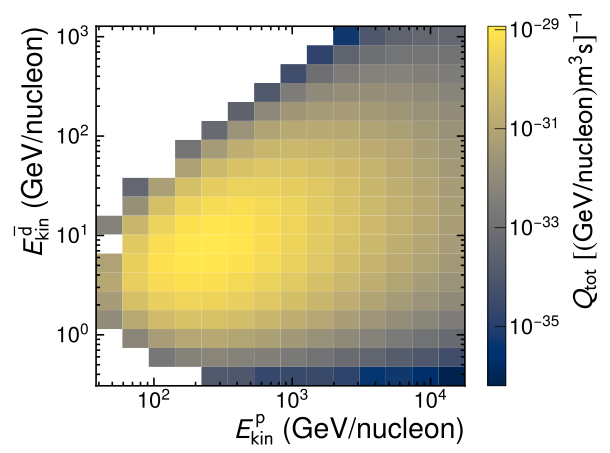
\includegraphics[width=0.37\textwidth]{figures/dbar_2dplot_production.png}
    \caption{(Left) Cosmic ray particle spectra, for protons and all particles, from relevant experiments. Figure taken from \cite{ThomasThesis}. (Right) the source term of antideuteron from high energy cosmic ray collisions, as a function of the incoming proton energy and the outgoing antideuteron energy. The figure is taken from \cite{dbar paper}.}
    \label{fig:CR_spectra_Thomas}
\end{figure}
%This whole section needs a rewrite. I need to mention:
% - Production cross sections for both antideuterons and anti-3He, with the plots, and discussing the difference between the two production models.
% - energy ranges for cosmic rays, and the shape of the produced spectra
% - Spectra of cosmic ray protons which might produce these antinuclei
% - talk about the data used to generate those production cross sections


\subsubsection{Weakly interacting massive particles (WIMPs) dark matter}\label{sec:WIMPS}
Some WIMP dark matter theories predict that WIMP annihilations can produce a significant amount of antinuclei \cite{}. Such theories are based on the assumption that dark matter is made of particles (hereinafter denoted $\chi$), which during the big bang were in thermal equilibrium with SM particles. This requires that some SM processes were able to create $\chi$. This can be understood kinematically from the available energy in such a process. If the SM particles colliding would have an energy which exceeds \Vs\ = $2\mathrm{m}_\chi$, they could create a dark matter particle pair. Similarly, the dark matter particles would have to be able to either decay or annihilate into SM particles, in order to maintain the equilibrium, as shown in figure \ref{fig:DM_ann_decay_processes}. We shall first consider the scenario that the dominant mechanism of interaction for dark matter into SM particles was decau. If they would only decay, there would have to be some mechanism which reduces this decay rate by many orders of magnitude once the thermal equilibrium is broken and dark matter decoupled from baryonic matter, since otherwise dark matter would have continued to decay rapidly and almost none would be left today\footnote{This would require a mechanism to destabilize dark matter particles in the very hot and dense medium which existed just after the big bang. During the period before dark matter decoupled -- which is assumed to have occurred around the quark-gluon-plasma phase of the early universe, i.e. $10^{-12}$s - $10^{-5}$ s after the big bang -- the decay rate would have had to be much less than $10^{-5}$s in order to achieve thermal equilibrium. In order to remain stable after decoupling, its lifetime would have to exceed the current lifetime of the universe, around $10^{17}$s. In medium modifications of decay widths is a known effect\cite{}, however, it is difficult to imagine a process which modifies the lifetime of such particles by at least 20 orders of magnitude.}. For dark matter annihilations no such effect is necessary, since the annihilation rate naturally decreases with the dark matter density squared (this will be explained in equation \ref{eq:DM_source_term}). Thus, as the universe expands, dark matter with a coupling into baryons through annihilation will naturally freeze out and its abundance from this point would remain almost constant. However, given that residual annihilations are still possible when two dark matter particles meet, any SM particles produced could be observed and shine a hint on its nature. It is this exact process which is looked for in cosmic ray antinuclei signals. A cold dark matter particle pair annihilating at rest has \Vs\ = $2\mathrm{m}_\chi$. The net baryon number would be 0 in such a process, resulting in no further penalty for the production of multiple antinucleons. Per definition, WIMPs interact only weakly, and thus their initial annihilation would occur through a weak channel. Since the weak bosons couple to all other standard model particles, this enables the production of particles such as antinuclei. \\
%(such as W$^+$W$^-$ or b$\overline{\mathrm{b}}$)

\begin{figure}[hbtp]
    \centering
    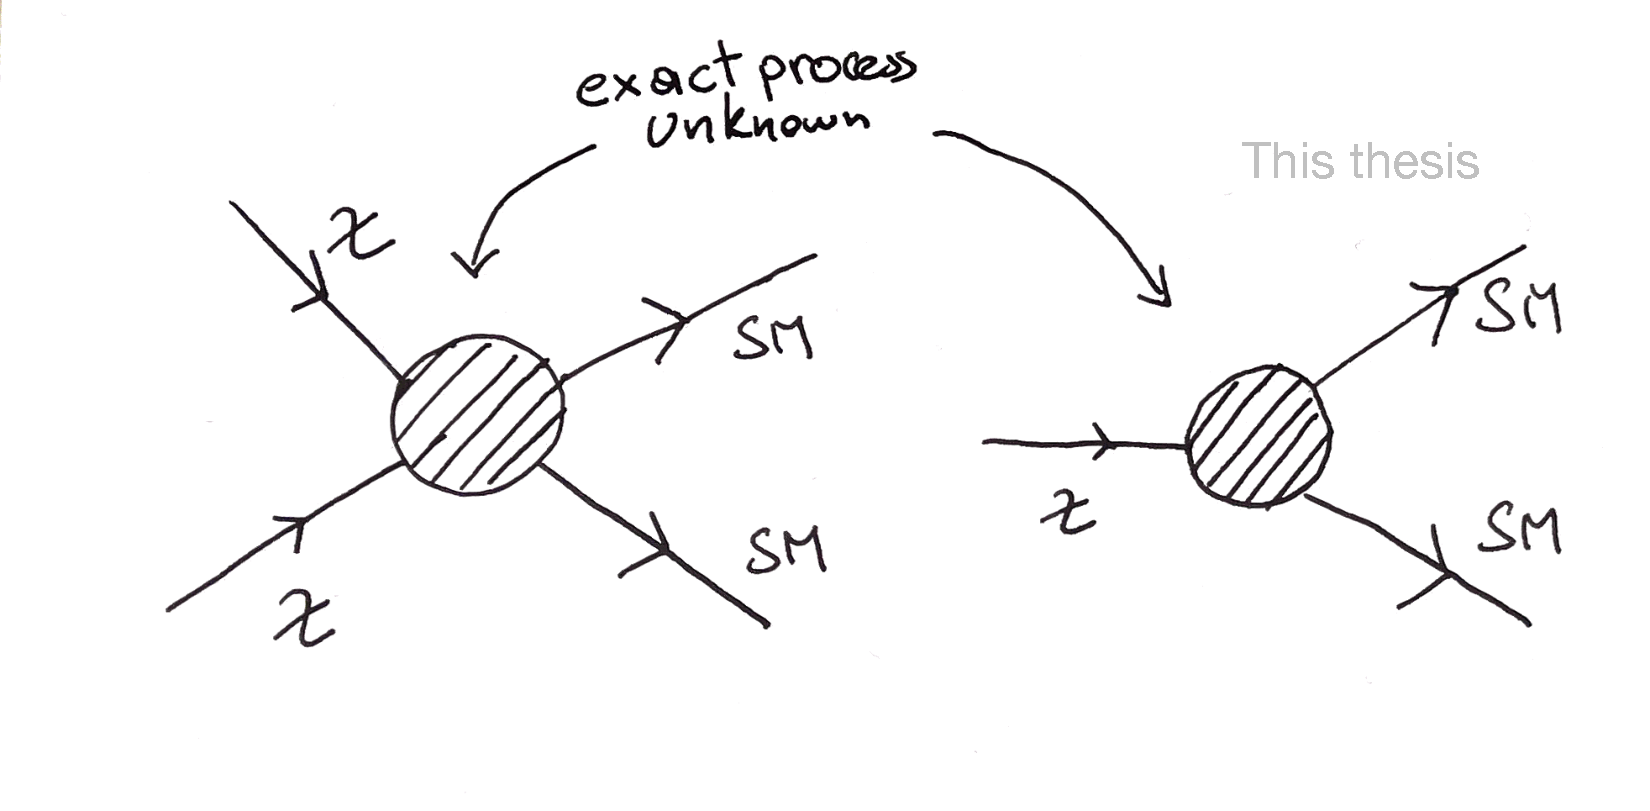
\includegraphics[width=\textwidth]{figures/DM_processes.pdf}
    \caption{A schematic of dark matter pair annihilation into standard model particles (left) and of dark matter decay into standard model particles (right) for a WIMP particle. The exact process by which this would occur is not known, and therefore currently model dependent. Note that a scattering process between a dark matter and a standard model particle would look very similar to the diagram on the left, with the space and time axes inverted (i.e. change the arrow direction of the top dark matter and bottom standard model particle). However, this scattering might happen via a very different internal process, so the two cannot be directly related in a model independent way.}
    \label{fig:DM_ann_decay_processes}
\end{figure}

The spectrum and yield of antinuclei produced in these annihilations has to be estimated based on known standard model processes. To this end, Monte Carlo event generators are employed\cite{}, in which the initial state is the first state of standard model particles which is assumed to occur in the annihilation process, with a COM energy equal to twice the dark matter mass \dmm \cite{cookbook}.%particle physics cookbook, also https://arxiv.org/pdf/hep-ph/9904481.pdf}. 
The exact initial state of SM particles is not known, but commonly the channels \WW\ and \bb\ are considered \cite{}. These two form a convinient subset, as over the range of expected masses (~10 GeV to about 1 TeV), they are consistently two of the more opimistic scenarios, and cover the different parameter space within these optimistic scenarios\cite{}. This can be seen from figure \ref{fig:DM_source_spectra_other_channels}. 
eince event generators do not produce (anti)nuclei -- but only the individual nucleons -- the (anti)nuclei yields and spectra have to be calculated using the coalescence model\footnote{See the appendix i\ref{App:statHadronModel} for an explaination for why the statistical hadronization model cannot be used to predict antinuclei spectra.}
The authors argue that while the branching ratio for the process $\overline{\Lambda}_b \rightarrow $ \ahe\ $+X$ is not well constrained by data, the default tunes\footnote{Tunes when used to talk to event generators are the specific settings which are used for the event generator to more accurately reproduce a given result, e.g. the proton spectra at a given energy.} of the event generators tends to underestimate this, and thus the amount of \ahe\ production (it also has an impact on the antideuteron production, but far less, as can be seen in section \ref{} below). In particular, the authors note a discrepancy between two commonly used event generators (Pythia\cite{} and EPOS\cite{}) of about X orders of magnitude. In order to rectify this, the authors suggest using a special setting of the Pythia event generator, to reproduce the branching fraction close to the one of EPOS. This setting is referred to as the $\overline{\Lambda}_b$ tune in the following discussion. According to their results, the authors note that there is an almost 100 fold increase in the resulting \ahe\ flux, in particular at high energies around X GeV. This is of particular interest since according to the authors, such an increase would cause a signal detectable by the AMS-02 experiment, with an event rate of about 1/year.  The authors also consider the decay of $\overline{\Lambda}_b$ through light intermediator particles, which provides a slightly different spectrum.\\
So in addition to the spectra obtained using default event generators from \cite{}, the spectra incorporating the $\overline{\Lambda}_b$ decay are also considered as part of this thesis. All the relevant spectra from these processes for antideuterons and \ahe\ are shown in figure \ref{fig:DMsource_spectra}. \\ 
\begin{figure}[hbpt]
    \centering
    \includegraphics[width=\textwidth]{figures/}
		\caption{Antiproton (top) and antideuteron (bottom) spectra from dark matter annihilations, normalized to a single annihilation event, for a wide variety of initial SM states. This figure is taken from \cite{cookbook}.}
    \label{fig:DMsource_spectra_other_channels}
\end{figure}
\begin{figure}[hbpt]
    \centering
    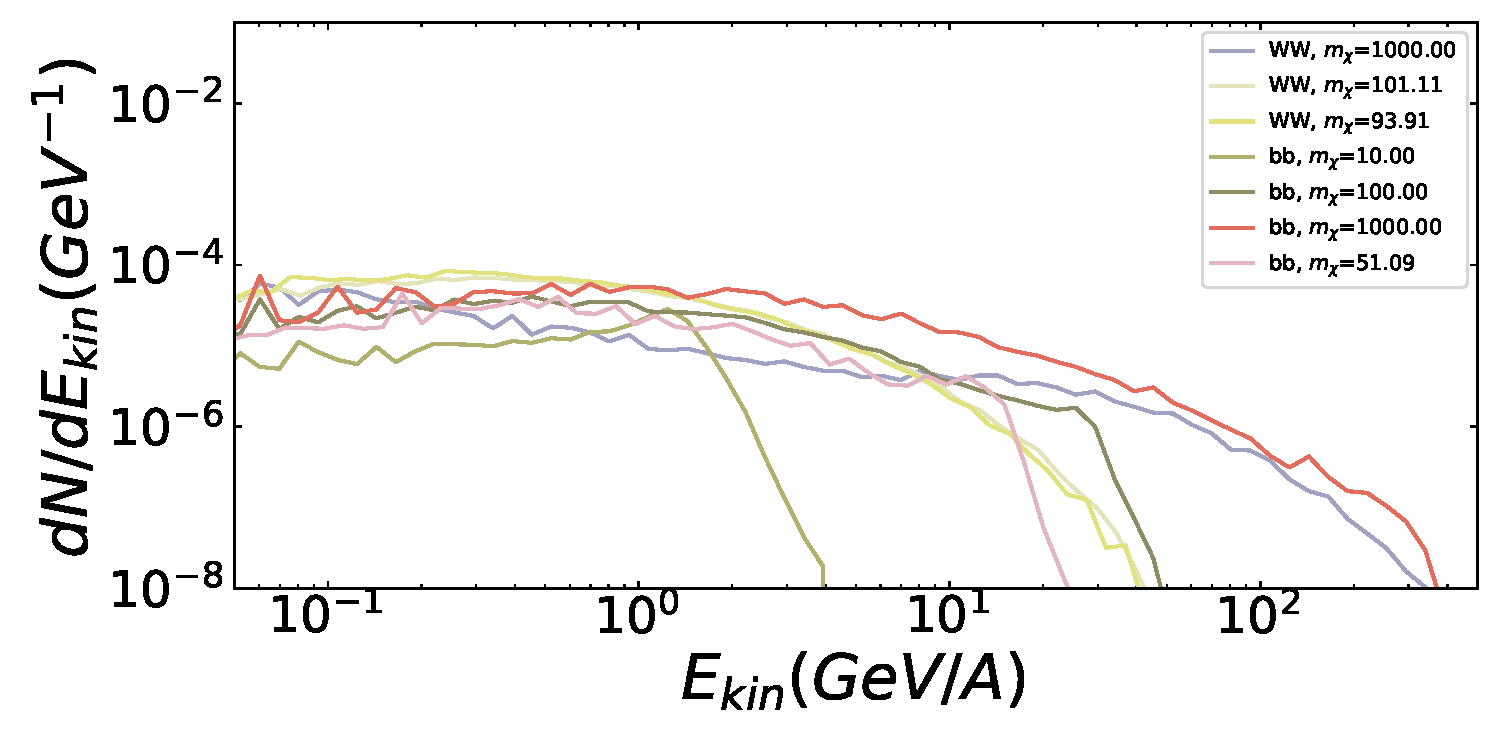
\includegraphics[width=0.45\textwidth]{figures/dbar_injectionSpectra.pdf}
    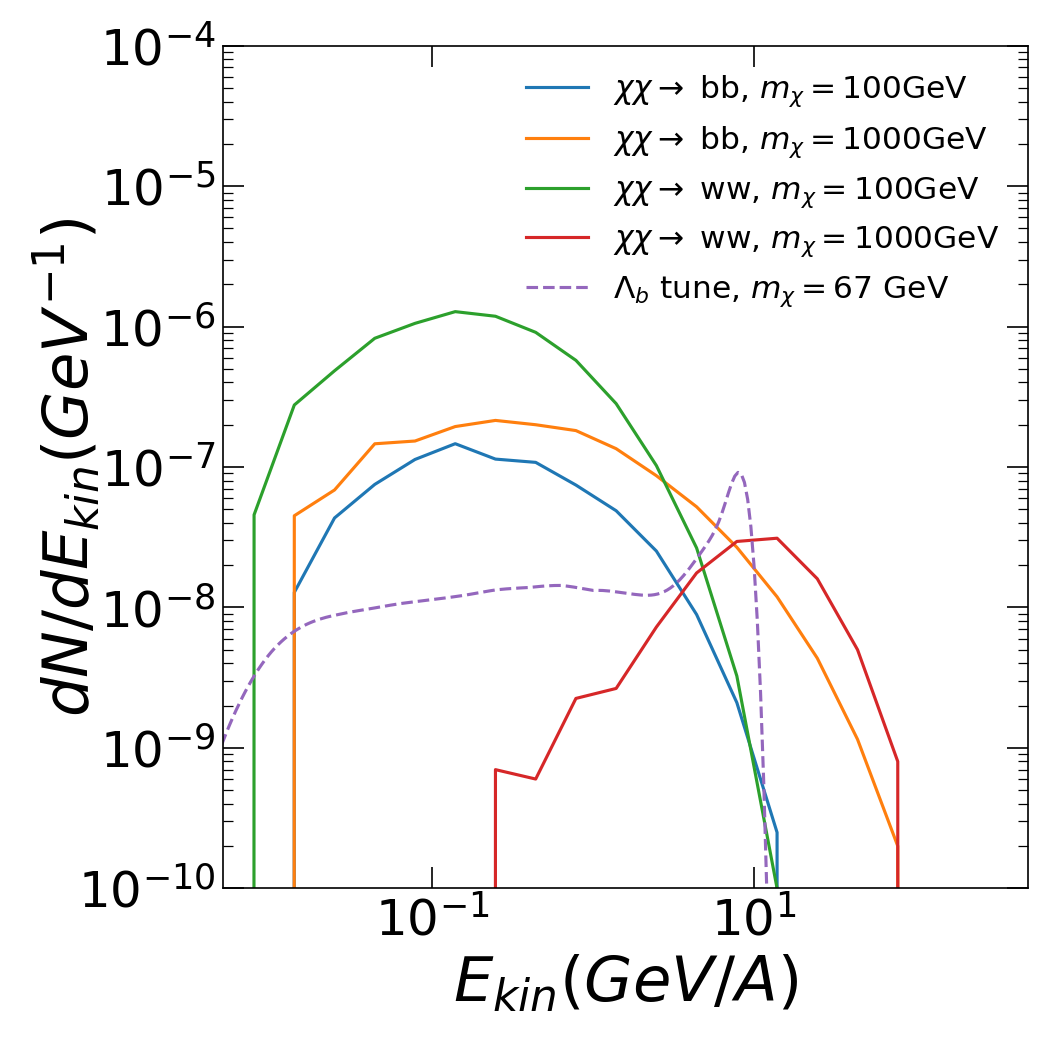
\includegraphics[width=0.45\textwidth]{figures/He3bar_injection_channels.png}
    \caption{Antideuteron (left) and \ahe\ (right) spectra from dark matter annihilations, normalized to a single annihilation event. Spectra for \WW\ \bb\ channels are taken from \cite{Ibarra:2012cc}, $\overline{\Lambda}_b$ tune is taken from \cite{}.}
    \label{fig:DMsource_spectra}
\end{figure}

%The WIMP dark matter is assumed to have been in thermal equilibrium with luminous matter after the Big Bang, and is believed to be responsible for the anisotropies seen in the cosmic microwave background (CMB) \cite{}. 
Since decoupling from baryonic matter, the dark matter would have cooled with the expanding universe, and thus is assumed to be at a similar temperature as the cosmic microwave background (CMB) today, of about 2.7K\cite{}. This is referred to as cold dark matter. Another consideration which supports cold dark matter is that the majority seems to be gravitationally bound within galaxies\cite{}. As such, the COM frame is assumed to be the same as the galactic frame, and no boost from the initial velocities are necessary. This is convenient, since one can therefore simply take the spectrum of produced antinuclei per dark matter annihilation -- which is obtained from applying a coalescence afterburner to the output of a Monte Carlo event generator -- and multiply it by the local annihilation rate of dark matter. Thus, one can write the source term $q(\vec{r}, E)$ for WIMP dark matter as: 

\begin{equation}\label{eq:DM_source_term}
    q(\vec{r}, E) = \frac{1}{2} \left( \frac{\rho_{\chi}(\vec{r})}{m_\chi}\right)^2 <\sigma v > (1+\epsilon) \frac{dN}{dE}
\end{equation}

where the factor $1/2$ comes from symmetry considerations for majorana dark matter\footnote{See section \ref{sec:IntroMajoranaDiracDM} for a discussion on the difference between Majorana and Dirac dark matter.}, the term $\left( \frac{\rho_{\chi}(\vec{r})}{m_\chi}\right)^2$ is the square of the number density of the WIMP dark matter, which is then multiplied by the velocity averaged dark matter annihilation cross section $<\sigma v>$, giving the rate of dark matter annihilations for a given point in space. The term 1+$\epsilon$ accounts for contributions from other particles which are produced and subsequently decay into the antinucleus in question, at timescales longer than the consideration of the MC event generator. The value of $\epsilon$ is 0 for antideuterons and 1 for for \ahe, to account for \atrit\ . The final term of equation \ref{eq:DM_source_term} is the spectrum of produced antinuclei normalised to a single dark matter annihilation. The terms of equation \ref{eq:DM_source_term}, their contraints and degeneracies are discussed below.\\

The dark matter density profile $\rho_\chi(\vec{r})$ affects both the total amount of antinuclei produced as well as their initial distribution. This parameter can be constrained from measurements of the Milky Way's rotation curve, similarly to how it is done for other galaxies. However, measuring the rotation curve of the Milky Way involves extra challenges, given that we are measuring from within. This is due to the fact that for other galaxies, measuring the difference in velocity through red/bluehisft at different positions is sufficient to measure the rotation curve, whereas for our own galaxies we need the measure both the 3d position and velocity of many stars. The most promising technique to do this is Very-Long-Baseline-Interferometry, which essentially uses telescope arrays spanning multiple continents as interferometers\cite{}. A more detailed discussion of measuring rotation curves can be found in \cite{Sofue_2016, Sofue2020}. Our galaxy's rotation curve  has been reported in \cite{Sofue2020}, found by combining multiple existing measurements. It is reproduced in figure \ref{fig:MilkyWayRotationCurve}. \\

\begin{figure}[hbtp]
    \centering
    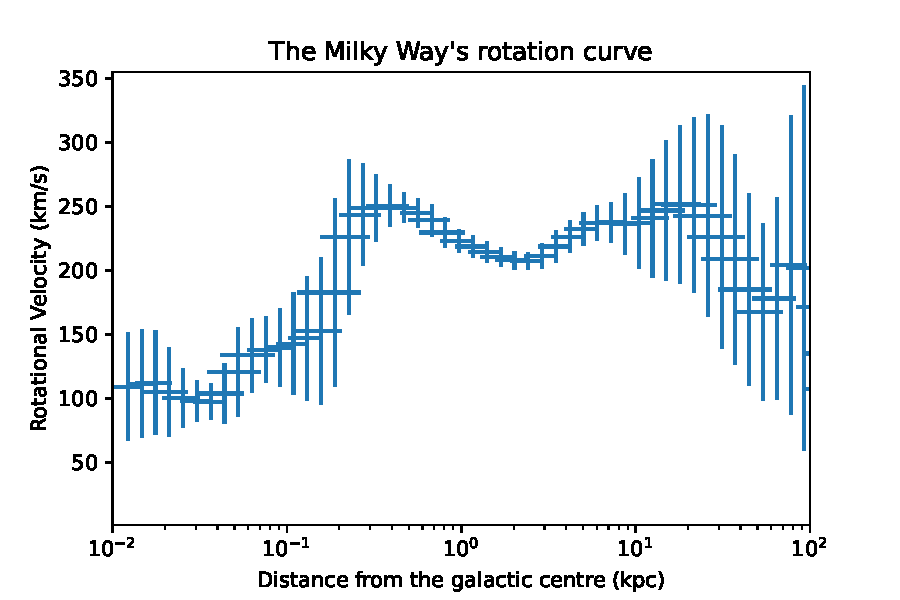
\includegraphics[width=\textwidth]{figures/RotationCurveMilkyWay.pdf}
    \caption{Rotation curve of stars in the Milky Way, as a function of distance from the galactic center. Reproduction of data reported in \cite{Sofue2020}.}
    \label{fig:MilkyWayRotationCurve}
\end{figure}

In order to fit such rotation curves, our galaxy is conventionally split into individual parts, each of which can be assumed to have a simpler shape. The usual breakdown of these parts is shown in table \ref*{tab:MilkyWayBreakdown}, and further details can be found in \cite{Sofue_2016}. The gravitational potentials of these parts can then be summed up linearly, and the rotational velocities caused by each such potential can be added in quadrature. In order to fit the contribution from dark matter, the shape of the dark matter distribution has to be chosen a priori, such that the exact parameters and normalization can then be obtained from the fit. This is an important point, since the total normalization of the dark matter profile is not well constrained. Rather, the relatively well constrained rotation curve in the proximity of the solar system results in the fact that the local dark matter density $\rho_\chi(\vec{r}=r_\odot) := \rho_\chi^\odot$ is much better constrained than the total normalization of the dark matter profile. Thus, the different dark matter profiles are constrained to their value at $r_\odot = 8.5$kpc\footnote{The value is currently estimated to be 0.4GeVcm$^-3$ \cite{}.}, the estimated position of our sun. \\
\begin{table}[h]
    \centering
    \begin{tabular}{|c|c|c|c|}
        \hline
        Part & Shape & Extent & Total Mass \\
        \hline
        Central black hole & Point mass & $<$ 0.1pc & 3.6$\times$ 10$^6$ M$\odot$ \\
        \hline
        Buldge(s) & Spherical exponential & $<$1kpc & 10$^{11}$ M$\odot$ \\
        \hline
        Flat disk & Constant flat disk & $<15$kpc & xx M$\odot$ \\
        \hline
        Dark matter halo & vaires & 100s of kpc & 10$^{12}$ M$\odot$ \\
        \hline
    \end{tabular}
    \label{tab:MilkyWayBreakdown}
    \caption{Individual axissymmetric parts of the Mikly Way used for fitting rotation curves. The distinction is made in order to simplify the fit, rather than a hard distinction within the actual galaxy. Non-axissymmetric components are neglected for rotation curves, based on the assumption that any effects would cancel out when averaged over the full rotation. The values for the total mass were taken from \cite{Sofue_2016}. The extent column is approximate and given in order to help the reader visualise the distributions. Due to the distributions being exponential, they only asymptotically approach 0.}

\end{table}

There are several profiles on the market, which achieve similar goodness-of-fit when fit to account for the dark matter component in the rotation curve\cite{}, while also achieving the required normalisation at $r_\odot$. The ones used in this work are the Navarro-Frenk-White(NFW) profile\cite{}, shown in equation \ref{eq:NFW}, 

\begin{equation}\label{eq:NFW}
    \rho_\chi^{NFW}(\vec{r}) = \frac{\rho_0}{(r/r_s)[1+(r/r_s)]^2}
\end{equation}
with scale radius $r_s=$24.42kpc, the Einasto profile\cite{}, shown in equation \ref{eq:Einasto}, 

\begin{equation}\label{eq:Einasto}
    \rho_\chi^{Einasto}(\vec{r}) = \rho_0 \mahtrm{exp} \left\{ -\frac{2}{\alpha}\left[ \left( \frac{r}{r_s}^\alpha -1\right) \right] \right\}
\end{equation}
with $\alpha$=0.17 and $r_s$=28.44kpc, and the much shallower isothermal profile \cite{} and the isothermal profile, shown in equation \ref{eq:isothermal}
\begin{equation}\label{eq:isothermal}
    \rho_\chi^{isothermal}(\vec{r}) = \frac{\rho_0}{r^2+r_s^2}
\end{equation}
with $r_s$=4.38kpc. The profiles are plotted in figure \ref{fig:DMProfiles}, using best fit values taken from \cite{Ibarra}. It can be seen that the isothermal profile has a very shallow rise towards the galactic center, while the Einasto profile rises very steeply. The NFW profile lies between the two\footnote{At very small radii, the NFW profile becomes larger than the Einasto profile.}, and is often used preferentially \cite{}. The stark difference between them is due to their origin. The isothermal profile is motivated purely by the fit to galactic rotation curves, while the NFW and Einasto profiles are motivated by the addition of numerical N-body simulations, which the isothermal profile struggles to replicate \cite{}. All these profiles assume spherical symmetry. Numerical simulations seem to prefer a triaxial ellipsoid, however, given the lack of data for the tidal motion of stars in the Milky Way, it is currently not possible to narrow down the shape more exactly than a simple spherically symmetric model. These three profiles cover most of the available parameter space for the dark matter profile. \\

\begin{figure}[hbtp]
    \centering
    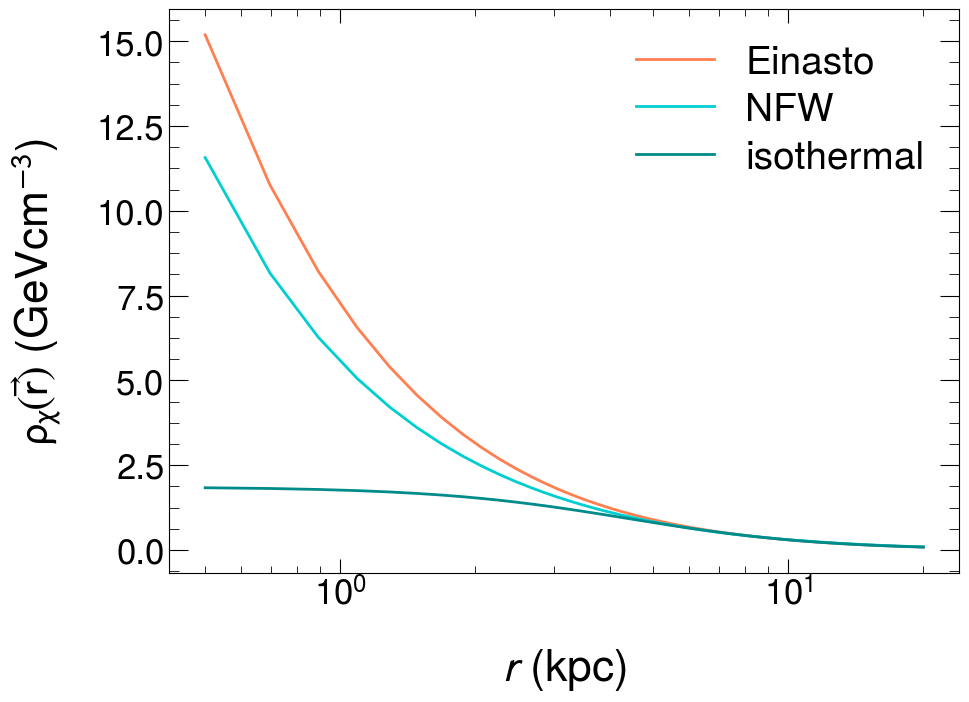
\includegraphics[width=0.8\textwidth]{figures/DMProfiles_distributions_log.png}
    \caption{Dark matter density profiles used in this work, as a function of the distance to the galactic centre. The best fit values for each profile are taken from \ref{Ibarra, IbarraSources}}
    \label{fig:DMProfiles}
\end{figure}

It is important to ask why the stark differences towards the center of the galaxy play such a reduced role that all three of these profiles are able to fit the data, and if such differences would therefore make any interpretation of an antinuclei flux from dark matter impossible. The answer to the first part of the question is twofold. Firstly, it is very challenging to measure the rotation curve of our own galaxy with high precision at positions far from the solar system, as can be seen from the uncertainties in figure \ref{fig:MilkyWayRotationCurve}. Secondly, the gravitational effect of the dark matter halo contributes mainly at distances larger than $\approx$ 2 kpc from the galactic center, where the presence of extra mass at the centre of our galaxy (from a steeper profile) is not as strongly felt. This can be seen from figure \ref{fig:RotationCurveFit}. The second question also has a fortunate answer: the effect of different profiles on a potential local flux of antinuclei from a dark matter source is rather small, as is discussed in section \ref{sec:ResDMProfiles}. 

\begin{figure}
    \centering
    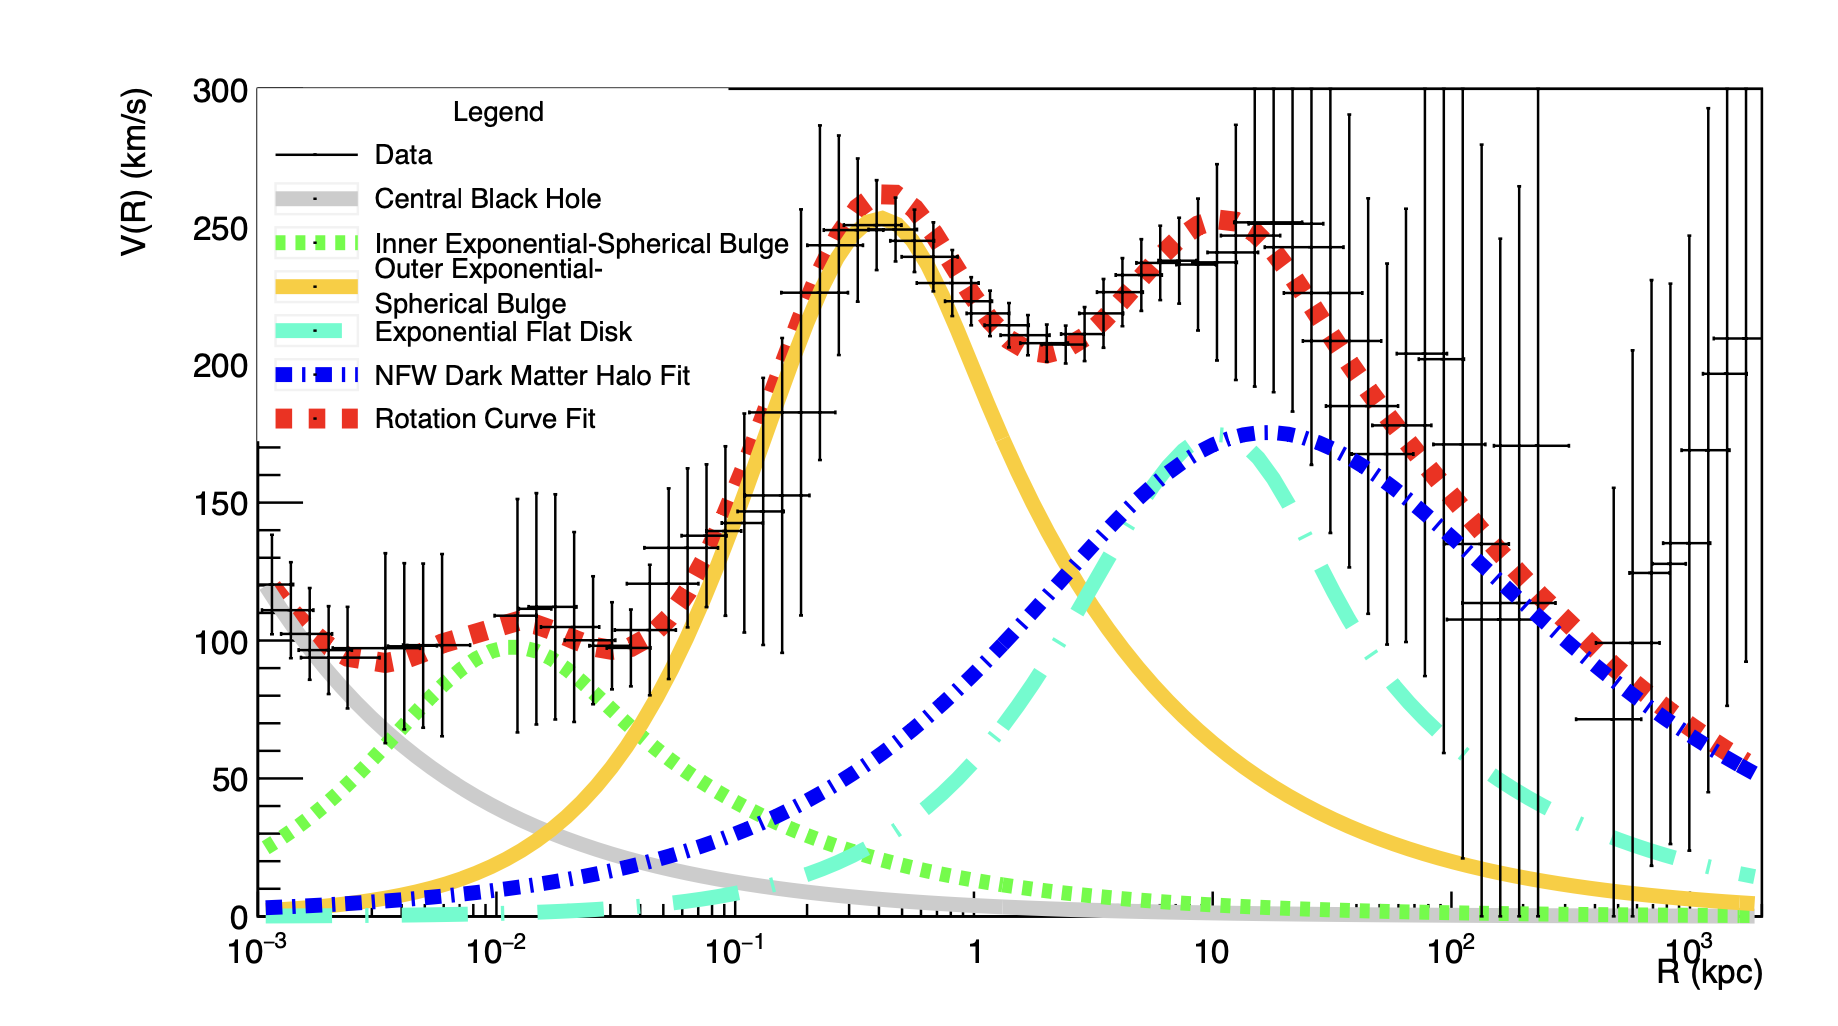
\includegraphics[width=\textwidth]{figures/Felix_rot_curve_fit.png}
    \caption{Fit of the rotation curve of the Milky Way, with a NFW profile. Figure is taken from \cite{Felix thesis}, based on work in \cite{}.}
    \label{fig:RotationCurveFit}
\end{figure}
To summarize: the dark matter density profile in our galaxy is constrained by measurements of the Milky Way's rotation curve. Measuring the rotation curve is a non-trivial process, which involves measuring the 3d position of stars within our own galaxy. The most modern method to achieve this is Very-Long-Baseline-Interferometry (VLBI), which uses telescope arrays spanning continents as a giant interferometer. Once the rotation curve is measured, the effect from luminous matter is accounted for, and the remainder is assigned to the dark matter component. Due to the experimental uncertainties involved in measuring the velocity of far away objects, this leaves a significant plausible parameter space for the shape of the dark matter profile towards the center of our galaxy. \\

The second term of equation \ref{eq:DM_source_term} is the dark matter mass, \dmm\ . The dark matter mass is a free parameter, with possible values ranging from very light dark matter\footnote{A popular light dark matter model is the axion model \cite{}.} below the eV range all the way to the WIMP dark matter discussed in this work, with plausible mass ranges from 10s of GeV to the TeV range. As discussed in section \ref{sec:IntroWIMPs}, the appeal of WIMP dark matter is that the expected weak cross section of such a particle in the very early universe would yield a population today of the same magnitude as we observe (a mathematical derivation can be found in \cite{dark matter production in the early universe} and is reproduced in section \ref{sec:IntroWIMPs}). It would also explain the lack of evidence for the production of dark matter at accelerators, since we might at this point not yet have reached the energies required to produce such particles. Finally, many extensions of the standard model naturally include such a particle, most notably super symmetry, which requires the neutralino, a particle which would fit the WIMP description\cite{}. This was a rather enticing argument at the inception of WIMPs in the 80s \cite{}, however, by now the parameter space for supersymmetric theories has become very small \cite{}, due to null observations at accelerators including the LHC \cite{}. This has made the question of how to incorporate such a particle into the Standard Model more difficult, and thus increased the interest in alternative dark matter candidates, which are discussed in section \ref{IntroOtherDM}.           

%\footnote{Additionally, some supersymmetric partners could have exactly these required properties, which would make them suitable dark matter candidates\cite{}. However, the lack of evidence for supersymmetry makes this argument somewhat weaker than it was during the inception of WIMPs \cite{}}. 

Since the exact nature of dark matter remains a mystery, a priori a wide range of masses is possible. However, direct detection experiments have placed limits on the dark matter-matter interaction cross sections, as a function of the dark matter mass \cite{} and a recent compilation of these limits is shown in figure \ref{fig:DirectDetectionLimits}. It is not possible to relate this interaction cross section with the dark matter self annihilation cross section $<\sigma_{ann} v>$ on general grounds, since they might depend on very different couplings. But it can help us make an informed decision on WIMP masses. As can be seen from figure \ref{fig:DirectDetectionLimits}, for masses over a few 10s of GeV, constraints become very strong, limiting the cross section to below a billionth of a pb. Upcoming next generation experiments, such as XENONnT\cite{} and Darkside20k\cite{}, are expected to push these limits within reach of the neutrino coherent scattering background. If these experiments also do not see a signal, it would eliminate the possibility of background free detection using direct detection methods. 

\begin{figure}
    \centering
    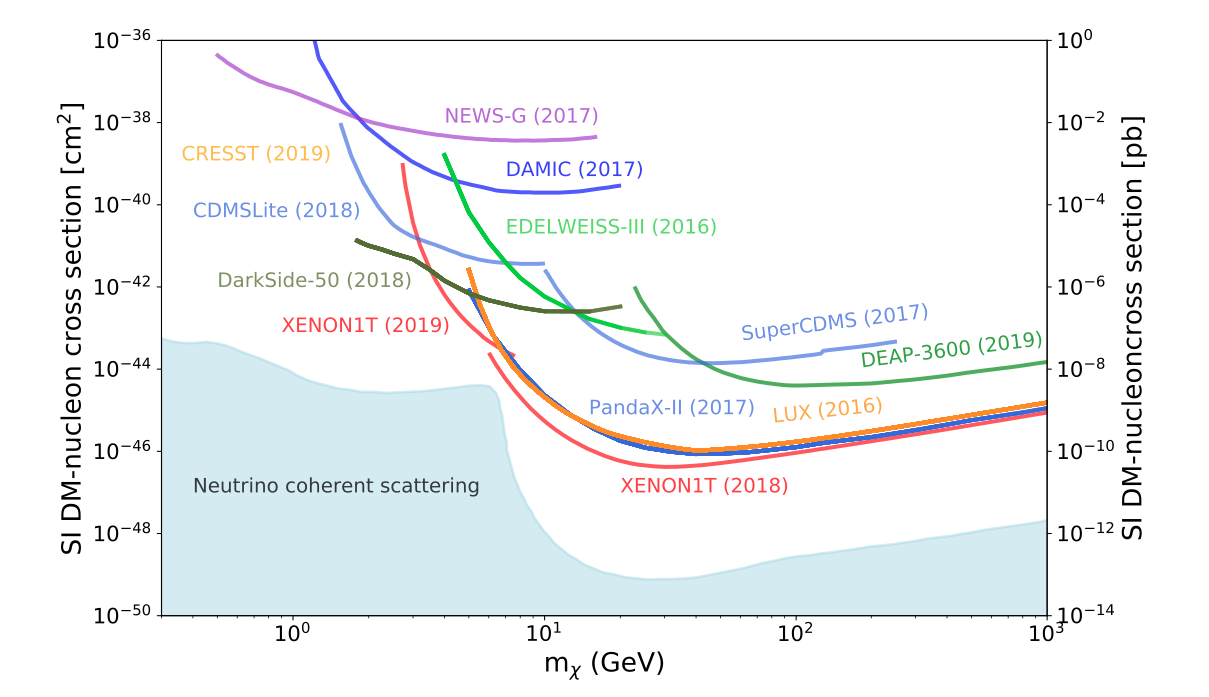
\includegraphics[width=\textwidth]{figures/Direct_detection_limits.png}
    \caption{Limits from direct detection experiments on the dark matter - nucleon interaction cross section, as a function of the dark matter mass. The figure is taken from \cite{Zyla_direct_detection}.}
    \label{fig:DirectDetectionLimits}
\end{figure}

The chosen mass has a direct effect on all three remaining terms of equation \ref{eq:DM_source_term}: i) $\frac{1}{m_\chi^2}$, ii) $\frac{dN_{\mathrm{\bar{p}, \bar{d}, {^3\overline{He}}}}}{dE}$  and iii)$<\sigma v>$. The effect on i) is trivial, and reduces the overall normalization of the antinuclei source term for higher \dmm\ . The mass' effect on ii) is based on the amount of energy available for the production of (anti)nuclei, as well as for their kinetic energy. For higher masses, the antinuclei yields increase non-trivially, but slower then the inverse square reduction from the first term. Additionally, the extra energy available for higher masses translates into a spectrum peaked at higher momenta. This depends not only on the available energy, but also on the decay channel. The $\frac{dN_{\mathrm{\bar{p}, \bar{d}, {^3\overline{He}}}}}{dE}$ spectra used for the antideuteron and \ahe\ results shown in this chapter are shown in figure \ref{fig:DMsource_spectra}. The effect of \dmm\ on $<\sigma v>$ is mostly experimental, since $<\sigma v>$ is constrained from antiproton measurements. 

Any dark matter annihilation process which can result in antideuterons must of course also produce antiprotons. However, contrary to heavier antinuclei, antiprotons are also copiously produced in other processes, due to the much lower energy threshold required for producing a single antinucleon, and the loss of the need to coalesce multiple antinucleons into a single compound antinucleus. This results in a significant and well constrained antiproton flux, which has been measured by the AMS collaboration \cite{}. Thus, any model chosen must not produce a dark matter component for antiprotons which is incompatible with those measurements. These limits are expressed in terms of $<\sigma v>$ as a function of \dmm\ . This representation is chosen since $\rho_\chi$ can be measured independently, and $<\sigma v>$ varies much more slowly with \dmm\ than the other terms. The limits -- which have been extracted by several groups \cite{} and compiled by \cite{}-- are shown in figure \ref{fig:DMSigmaVLimits}. Indicated in the figure is the maximum limit on $<\sigma v>$, as well as the thermal relic cross section ($\approx 1pb \times c$)\footnote{See the derivation in section \ref{sec:IntroWIMPs} for more details.}. 

Also indicated in this figure is the region in which a possible excess of antiprotons was observed in the \pbar\ spectrum measured by the AMS collaboration, which could hint at a dark matter particle within this mass range of 50-100GeV/$c^2$. It can be seen from the left hand side of the figure that for low dark matter masses, the limits lie significantly below the thermal value for this cross section. Thus, \dmm\ affects the constraints on  $<\sigma v>$, particularly for low masses. It is also worth noting that these limits have to be extracted for a given dark matter density profile, and thus when exploring the maximum allowed antinuclei flux given the antiproton constraints, the choice of $\rho_\chi(\vec{r})$ is degenerate with the limits on $<\sigma v>$ set by the AMS antiproton limits.\\

\begin{figure}[hbtp]
    \centering
    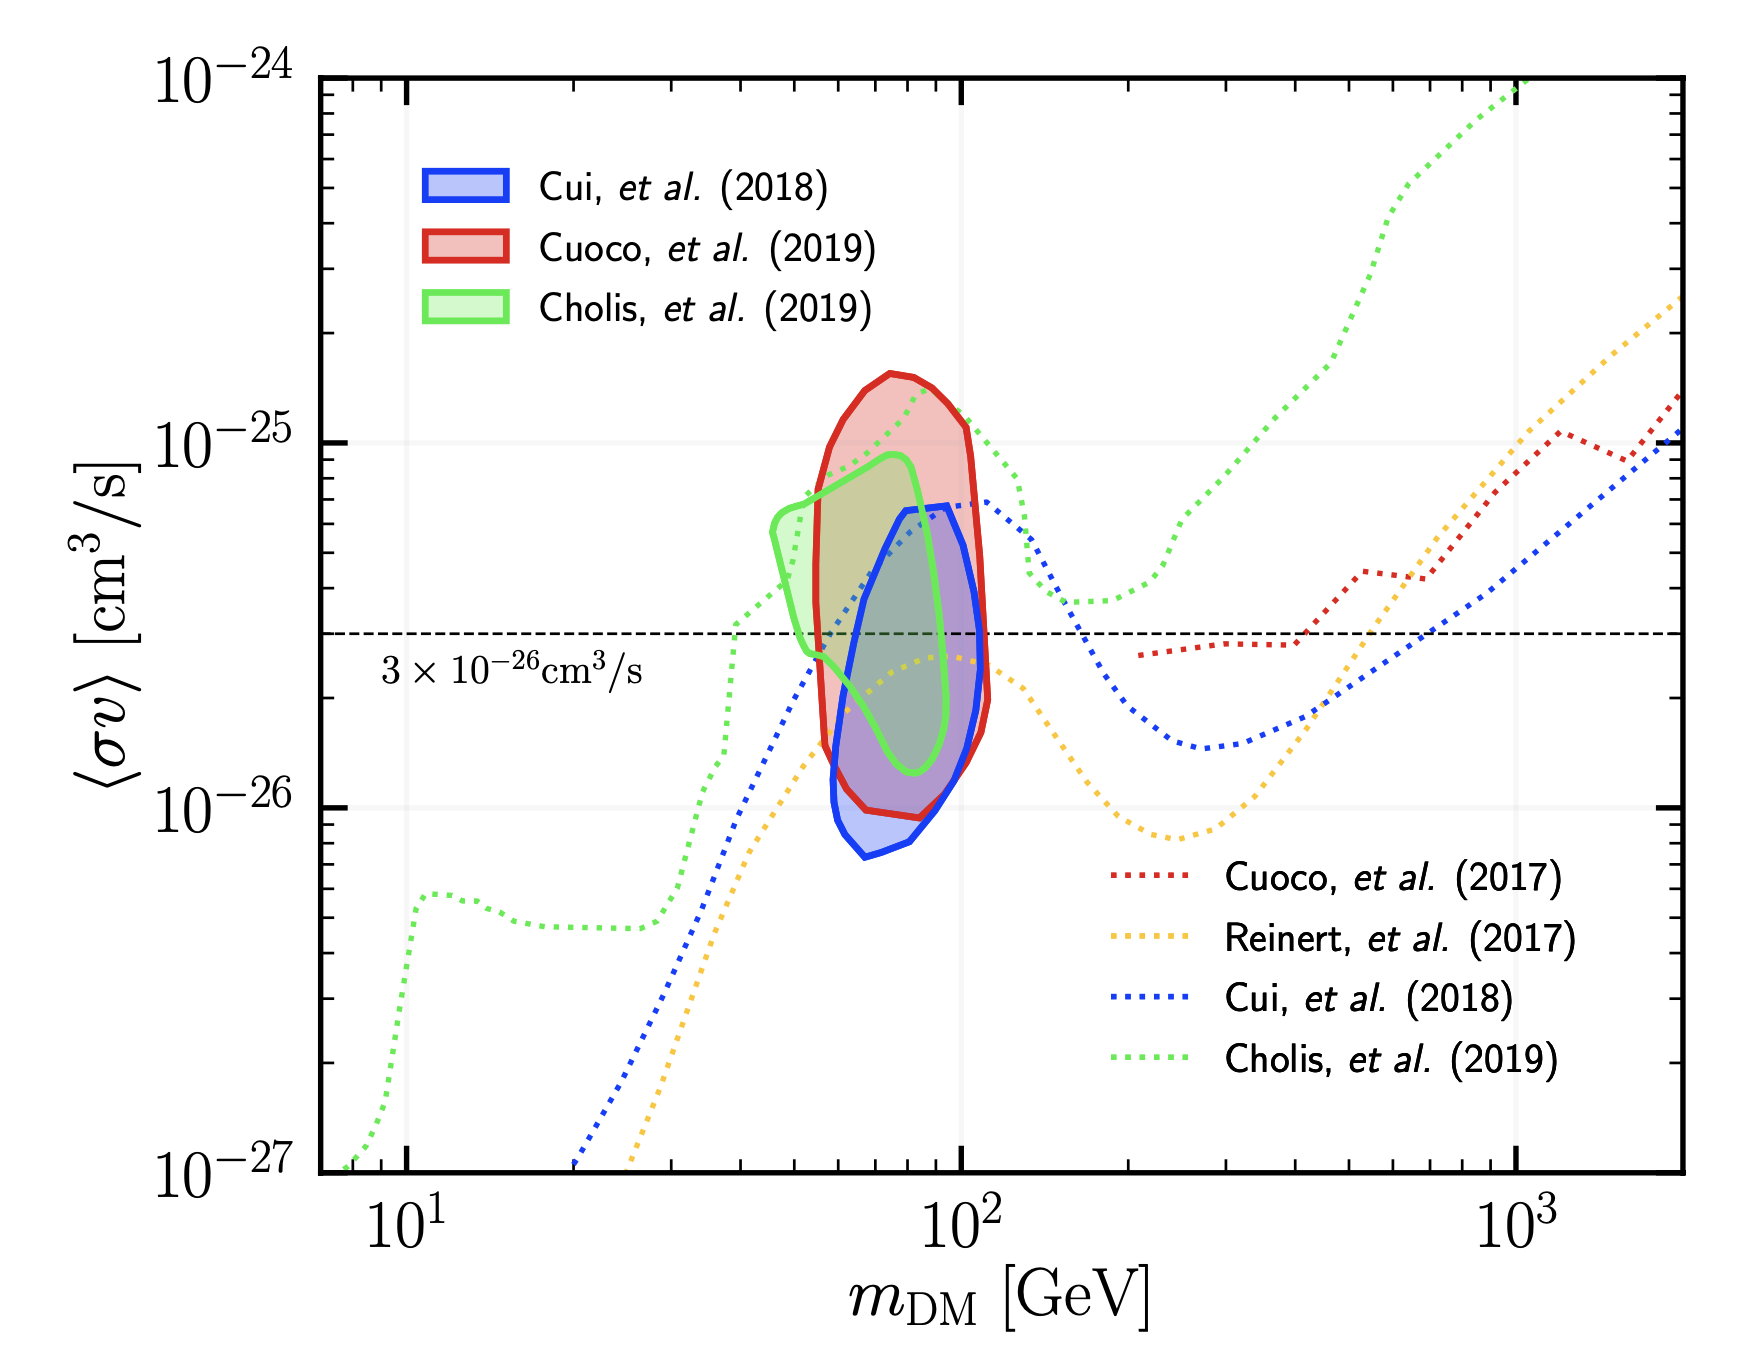
\includegraphics[width=0.8\textwidth]{figures/PbarLimitsAMS.png}
    \caption{Limits on  $<\sigma v>$ based on AMS antiproton data. Figure is taken from \cite{}.}
    \label{fig:DMSigmaVLimits}
\end{figure}

To summarise: WIMP dark matter models predict that dark matter can annihilate and produce antinuclei. The resulting antinuclei source term depends on 4 things: i) the dark matter density profile, ii) the dark matter mass, iii) the dark matter self-annihilation cross section and iv) the produced spectrum of antinuclei, normalised to a single dark matter decay. i) is constrained by looking at the rotation curve of our galaxy, ii) is a free parameter, iii) is constrained from above by antiproton measurements as a function of \dmm\ and iv) is calculated based on coalescence models, which depend on the total available energy and thus \dmm\ . Thus, there are a few notable degeneracies between the different terms of this source function. However, current constraints on these parameters are not stringent and leave open a large, reasonable parameter space which could result in a measureable antinuclei flux from a dark matter source, affirming antinuclei studies as a great tool for the indirect search for dark matter.



\subsubsection{Extragalactic dark matter}
Dark matter is not exclusively bound within galaxies, but is also present in larger cosmological structures, such as galaxy groups\cite{}. However, the profiles commonly used in order to fit the distribution of dark matter within our galaxy only take into account galactic dark matter, which can be inferred from the fact that such profiles go to 0 at large distances from the galactic centre. This is because to first order, the extragalactic component will vary over length scales bigger than our galaxy, so the gravitational potential caused by the extragalactic dark matter will be roughly constant within our galaxy, thus causing no active force which could be measured. However, such an additional flux of dark matter could indeed annihilate within our galaxy, thus providing an additional source for antinuclei. In this section the difference of this source to the galactic WIMP dark matter source will be qualitatively discussed. Previous work on the topic expects the extragalactic dark matter component to make up about 12\% of the local dark matter abundance close to our solar system\cite{}. From this, it can be estimated that the extragalactic dark matter is responsible for no more than $\approx 20$\% of the antinuclei flux near earth. \\ 

In order to determine whether the antinuclei flux caused by extragalactic dark matter follows the same assumptions as the galactic component, it is necessary to examine the differences between galactic and extragalactic dark matter. The first difference would be their velocity. Since the galactic component is bound and the extragalactic is not, the extragalactic component's velocity must exceed the escape velocity of the Milky Way, which lies at about 600km/s. This change in velocity may affect 2 terms in equation \ref{eq:DM_source_term}: the self annihilation cross section and the spectrum of produced antinuclei due to the boosted frame in which the collision takes place. \\
Starting with the effect on the self annihilation cross section, the difference might be due to the momentum dependence of the s-wave and p-wave contributions. The s-wave is velocity independent, while the p-wave contribution has a square dependence on the velocity. However, the speeds of 600km/s still only equate to a beta of 0.002, thus the contribution of the s-wave still dominates at these speeds, resulting in no change in regards to galactic dark matter. In a similar fashion it can be shown that the effect of the increased speed on the produced antinuclei spectrum is negligible. \\

The effect which remains is that of the overall normalisation, which is influenced by the extragalactic component to $\rho_\chi$. This extra component would have little to no effect on the rotation curve of our galaxy, and therefore causes a positive offset in comparison to the purely galactic case. The exact nature of this offset should to first order be roughly constant over our galaxy, however, the interaction of the extragalactic dark matter with our galaxy's gravitational pull would cause an increase in the local extragalactic dark matter density in comparison to another point within the local group. Thus, the main difference between the extragalactic dark matter and the galactic dark matter is the consideration of where the majority of annihilations would occur. Finally, we can conclude that since the overall normalisation for antinuclei fluxes from dark matter annihilations is constrained by the maximal allowed flux from antiprotons -- as discussed in section \ref{sec:WIMPS} -- the increase in flux due to an additional extragalactic dark matter component does not significantly impact expectations. \\

\subsubsection{Primordial black holes}
Another possible source of antinuclei in the cosmos are primordial black holes (PBHs). These objects would have formed very early in the universe, created from overdense regions shortly after the big bang. Their mass is therefore given by the particle horizon at the time of formation, $M_\mathrm{PBH} \approx c^3t/G \approx 10^{15} (t/10^{-23}s)g$ \cite{}, where $t$ is the time at their formation. These objects can have a large range in different masses, depending on their formation time. Since such low mass black holes would interact only gravitationally, they would meet the criteria for dark matter \cite{}. However, as we shall see in this section, they cannot make up the dominant portion of dark matter in the galaxy. \\
Classically, it is impossible for anything - even light - to escape a black hole. However, as shown by \cite{}, quantum mechanics predicts that black holes will indeed thermally emit (anti)particles, with a characteristic temperature $T = \frac{\hbar c^3}{8\pi GM k_B} \approxeq 1.06 \left( \frac{M}{10^{13}g}\right)^{-1} \mathrm{GeV} k_b^{-1}$ \cite{}. This process can be understood as particles tunneling out of the black hole\cite{}, or as virtual antiparticle-particle pairs being created and one partner tunneling through the event horizon into the black hole, preventing recombination \cite{}. Both methods yield the same results. The lifetime of such black holes scales with their mass as $\tau_\mathrm{PBH} \propto M_\mathrm{PBH}^{-3}$, i.e. they evaporate faster the smaller they are. This results in PBHs emitting many (anti)particles almost simultaneously when they fully evaporate at the end of their lifespan, a process akin to an explosion. The mass of currently evaporating PBHs is in the range of about $\approx 10^{15}g$, since lighter black holes would have already evaporated in the past, while heavier ones will only evaporate in the future. Such PBHs could produce antinuclei during the final stage of their evaporation. //
The current abundance of PBHs in this mass range is most tightly constrained from $\gamma$-ray searches\cite{}, to $\frac{\rho_\mathrm{PBH}}{\rho_\mathrm{tot}} < 10^{-26} (M_\mathrm{PBH}/10^{15}g)^{-5/2}$, which means that PBHs cannot make up all the dark matter in our galaxy. These limits include the extragalactic gamma ray background (for masses down to $10^{13}g$) and the galactic gamma ray spectrum (for masses of $\approx 10^{15}g$).\\

In this thesis PBHs were considered as a possible source for antideuterons, using a PBH mass of $9.35\times 10^{14}g$. For this mass, PBHs were found from antiproton constraints to make up no more than $f_\mathrm{PBH} = 4\times 10^{-11}$ of all the dark matter in the galaxy. This corresponds to a local rate of PBH explosions of $2\times 10^{-4} pc^{-3}yr^{-1}$. The source term of antideuterons from such events is given by equation \ref{eq:pbh_source_term},

\begin{equation}\label{eq:pbh_source_term}
		q ( \vec{r}, p) = \frac{f_\mathrm{PBH} \rho_{\mathrm{CDM}} (\vec{r})}{M_\mathrm{spectrum}}\frac{dN}{dT}

\end{equation}
, where $M_\mathrm{spectrum}$ is the typical mass of the PBHs considered, and $\rho_\mathrm{CDM}$ is the cold dark matter density profile, equivalent to the one used for WIMPs. The corresponging antideuteron spectrum per second $\frac{dN}{dT}$ is taken from \cite{}, and is shown in figure \ref{fig:pbh_source_spectrum}.

\begin{figure}[hbtp]
		\centering
		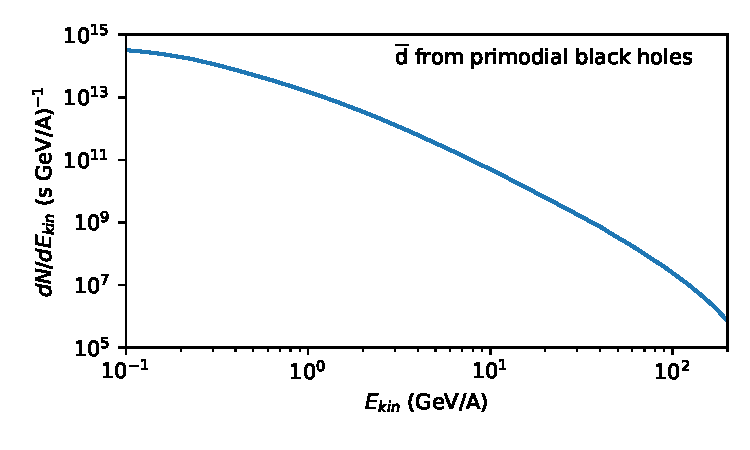
\includegraphics[width=0.99\textwidth]{figures/pbh_source_spectrum_dbar.pdf}
		\label{fig:pbh_source_spectrum}
		\caption{Spectrum of produced antideuterons per second from a primordial black hole evaporation, taken from \cite{}.}
\end{figure}



\subsection{Constraining the propagation of antinuclei through the galaxy}\label{sec:Propagation}
In the process of propagating thorough our galaxy, particles undergo several different effects. They get produced at various points in both space and time, for example most heavy nuclei are produced in supernovae\cite{}. As they then propagate from their source towards their eventual detection point near earth, they undergo diffusion effects, undergo elastically scattered and are diverted by the magnetic fields of the galaxy and individual celestial objects. They are also under the effect of bulk motion via convection effects. Finally, there are various effects which might cause a particle to disappear, mainly inelastic interactions with the interstellar medium, or breakup for unstable particles. All of these processes are characterised by the transport equation \cite{}, which is reproduced in equation \ref{eq:TransportEquation}
\begin{equation}
    \label{eq:TransportEquation}
    \frac{\partial\psi}{dt} = q(\textbf{r},p) + \mathrm{\textbf{div}}(D_{xx}\mathrm{\textbf{grad}}\psi - \textbf{V}\psi) + \frac{\partial}{\partial p}p^2D_{pp} \frac{\partial}{\partial p}\frac{\psi}{p^2} - \frac{\partial}{\partial p} \left[ \psi \frac{dp}{d t}   -\frac{p}{3} (\mathrm{\textbf{div}}\cdot  \mathrm{\textbf{V}} )\psi              \right] \\ - \frac{\psi}{\tau_f}-\frac{\psi}{\tau_r}
\end{equation}
, where $\psi$ is the time and space dependent flux of a given cosmic ray species, $q(\textbf{r},p)$ is the source term as a function of position and momentum, $D_{xx}$and $D_{pp}$ are the spatial diffusion and diffusive re-acceleration coefficients, $V$ is the convection velocity, and $\tau_f$ and $\tau_r$ are parameters characterising the annihilation and fragmentation rates, respectively. The relationship between the last term and the inelastic cross section of a cosmic ray species is given by: 

\begin{equation}\label{eq:annihilation_lossTerm_relation}
    \frac{1}{\tau_r} = \beta c \left( n_\mathrm{H}(\vec{r})\sigma_{\mathrm{inel}}^{^3\mathrm{\overline{He}p}} (p) + n_{\mathrm{He}}(\vec{r})\sigma_{\mathrm{inel}}^{^3\mathrm{\overline{He}^4He} (p)} 
    \right)
\end{equation},
where, $n_\mathrm{H}$ is the number density of hydrogen gas (approximately 1 m$^{-3}$), $n_\mathrm{He}$ is the number density of helium gas (approximately 0.1 m$^{-3}$). \\%These values vary slightly throughout the galaxy by about XX\%. This is taken into account in the propagation in GALPROP. 

Equation \ref{eq:TransportEquation} can be solved for a given set of parameters both analytically or numerically. Several tools exits in order to solve this equation, with the most well known being GALPROP\cite{}, Dragon \cite{} and PICARD\cite{}. In this work, GALPROP was used, which solves the transport equation numerically and will be explained in section \ref{sec:GALPROP}. Galprop uses astrophysical measurements for the interstellar gas and cosmic ray source distributions, and employs nuclear physics measurements for interaction cross sections of particles and nuclei. Many different particle species can be en- or disabled in GALPROP, which affects the runtime of the simulations. For antinuclei from dark matter, other species need not be included, since the result is independent of other particle species. However, for antinuclei from secondary cosmic rays, other cosmic ray species can affect the total flux and therefore need to be considered.\\

It is important to note that only the first and final term of equation \ref{eq:TransportEquation} -- i.e. the source and loss terms -- depend on the species of particle which is being considered. The other terms, which cover the actual propagation through the galaxy, depend solely on parameters which are common to all particle species. This can be understood as the same magnetic fields and bulk motion affecting all particles. Thus, these parameters can be constrained by fitting abundant cosmic ray species which are sensitive to a particular parameter, in order to constrain the propagation for all species. This is particularly important for the propagation of antinuclei, which are extremely rare. These propagation parameters have been investigated and reported by e.g. Boscini\cite{} and Cuoco \cite{}. The effectiveness of these fits can be seen by comparing predicted spectra of protons, antiprotons and heaver cosmic ray nuclei with the measurements done by AMS-02, which are shown in figure \ref{fig:BosciniFits}. The solid lines are the predictions from the Boscini model after solar modulation is applied, while the dashed lines are the predictions before solar modulation. It can be seen that the predictions work very well for large energies, and there is a smooth response at low energies, which is well understood based on the effects of the heliosphere. This shows that the propagation is well under control.\\

\begin{figure}[hbtp]
    \centering
    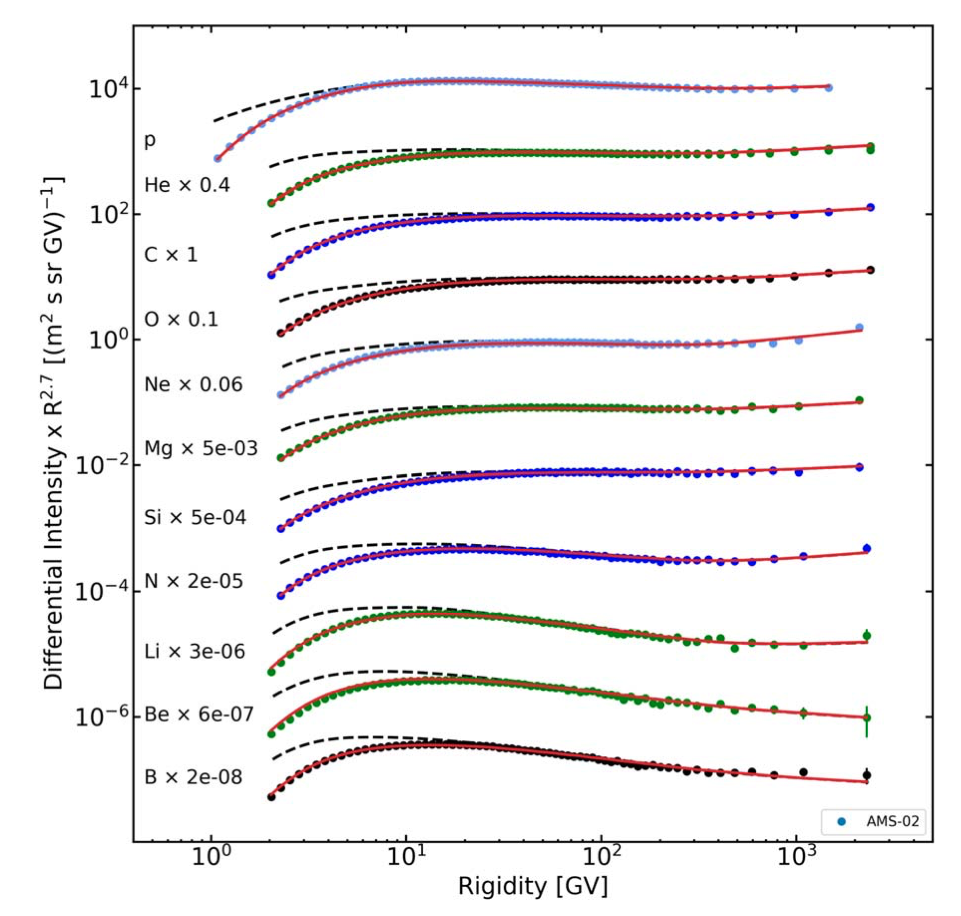
\includegraphics[width=0.8\textwidth]{figures/Boscini_Fits.png}
    \caption{Fluxes of several cosmic ray nuclei, as measured by AMS-02, compared to the predictions of the best-fit values obtained by fitting several key species. Figure taken from \cite{Boschini:2018baj}}
    \label{fig:BosciniFits}
\end{figure}

The effect at low energies is due to the effect of the heliosphere, which is not included in codes such as GALPROP. These codes can only simulate large scale effects, and as such they output the particle fluxes outside of our solar system. Within our solar system, the solar magnetic field will affect incoming charged particles, and this needs to be accounted for. The solar mangnetic field is not constant, but rather it varies over an 11 year period\cite{}. Thus, the effect of the solar modulation is also time dependent and needs to be calculated for a specific scenario. In this thesis, a solar minimum is considered, in order to discern the most optimistic flux of low energy antinuclei. There are tools which treat this in great detail for cosmic rays, such as HELMOD \cite{}, but there are currently no such tools on the market which are able to treat antinuclei. Thus, a simple force field model has been commonly used for this purpose in the literature \cite{}. The advantage of this model is its broad applicability, while its disadvantage is mainly a large uncertainty induced for low momentum particles\cite{}. The force field model is a simplified solution to the Parker equation \cite{29 from CR AN}, which treats the full extent of the problem including solar winds and turbulences. This complete treatment relies on knowledge of turbulences and boundary spectra of the particle species involved, and thus lies beyond the scope of this thesis and similar analyses \cite{Korseier 2018, Ibarra, Boschini:2018baj}. The force field approximation reproduces the overall effect of solar modulation, although the exact values it produces are not exact at low energies \cite{}. It also relies only on a single parameter, the so called Fisk potential $\phi_F$, and related the unmodulated flux $F$ to the modulated flux $F'$ according to equation \ref{eq:ForceFieldFlux}, while modifying the corresponding kinetic energies according to equation \ref{eq:ForceFieldEnergies}

\begin{equation}
    \label{eq:ForceFieldFlux}
    F' (E', \phi) = F(E) \frac{(E-Z\phi)^2 - m^2}{E^2-m^2}
\end{equation}

\begin{equation}
    \label{eq:ForceFieldEnergies}
    E' = E-Z\phi
\end{equation}
, where $m$ denotes the mass of the cosmic ray species in question. For the analyses in this thesis, the Fisk potential is assigned a value of 0.4 GV. \\

It is important to note that some of the propagation parameters which are degenerate for one source are not necessarily so for another. In particular, the source from dark matter is strongly dependent on the height of the galaxy considered (since this increases the total amount of dark matter considered), rather than the ratio of the diffusion and the height, $D_{xx}/z_h$, which is the common factor for antinuclei from high-energy cosmic rays. This degeneracy for secondaries can be seen in table \ref{tab:GalpropParameters}, where the aforementioned  ratio is shown to be consistent between the two paramterizations. Since propagation parameters are constrained by nuclei following roughly the same source distribution as secondaries, this difference in sensitivity causes a much larger uncertainty in the possible fluxes for antinuclei from dark matter than for antinuclei fluxes from high-energy cosmic rays. \cite{}. This is also shown in figure \ref{fig:ComparisonPropagation}, where it can be seen that for a wide energy range, both different propagation parameterization used in this work give near identical antideuteron fluxes from high energy cosmic ray collisions, while for dark matter the difference is more than a factor 2. For antideuterons from high-energy cosmic rays the discrepancies between the two different parameterizations only become non-negligible at very low energies, where the propagation is less well constrained and complicated by the need to disentangle solar modulation effects. 

\begin{figure}[hbtp]
    \centering
    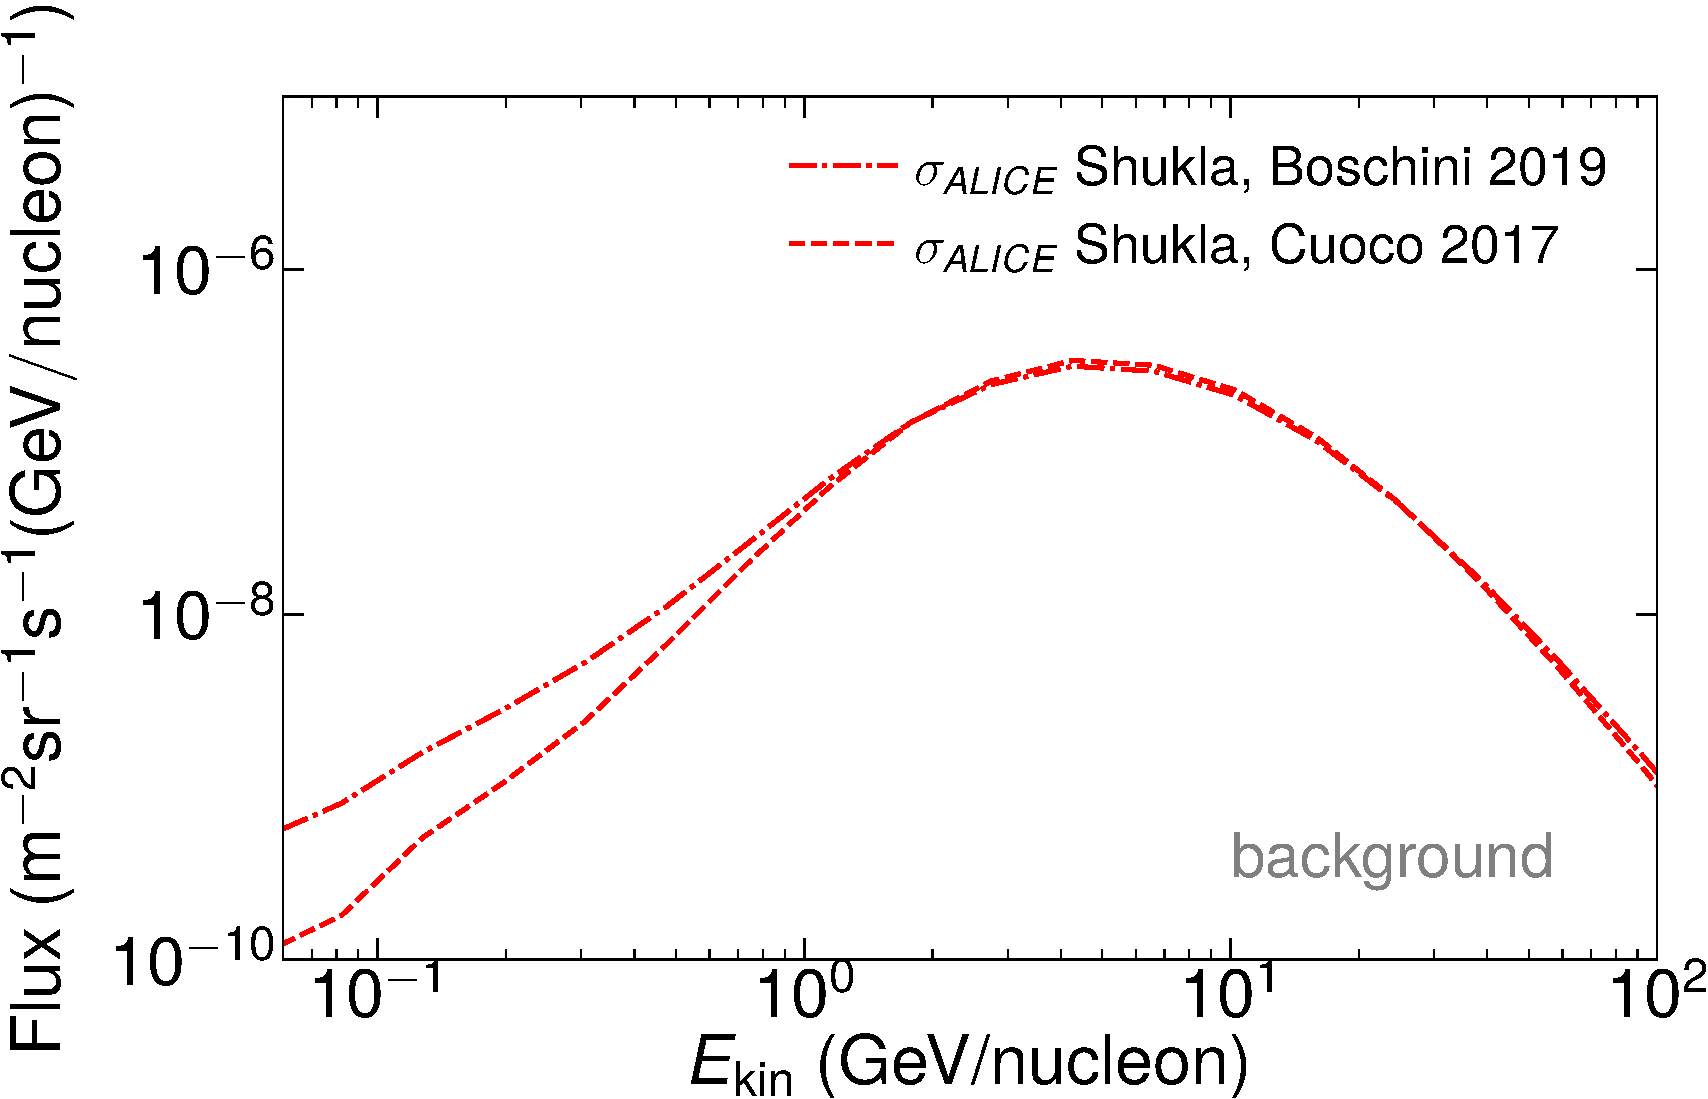
\includegraphics[width=0.48\textwidth]{figures/ComparisonPropagationBoschini.pdf}
    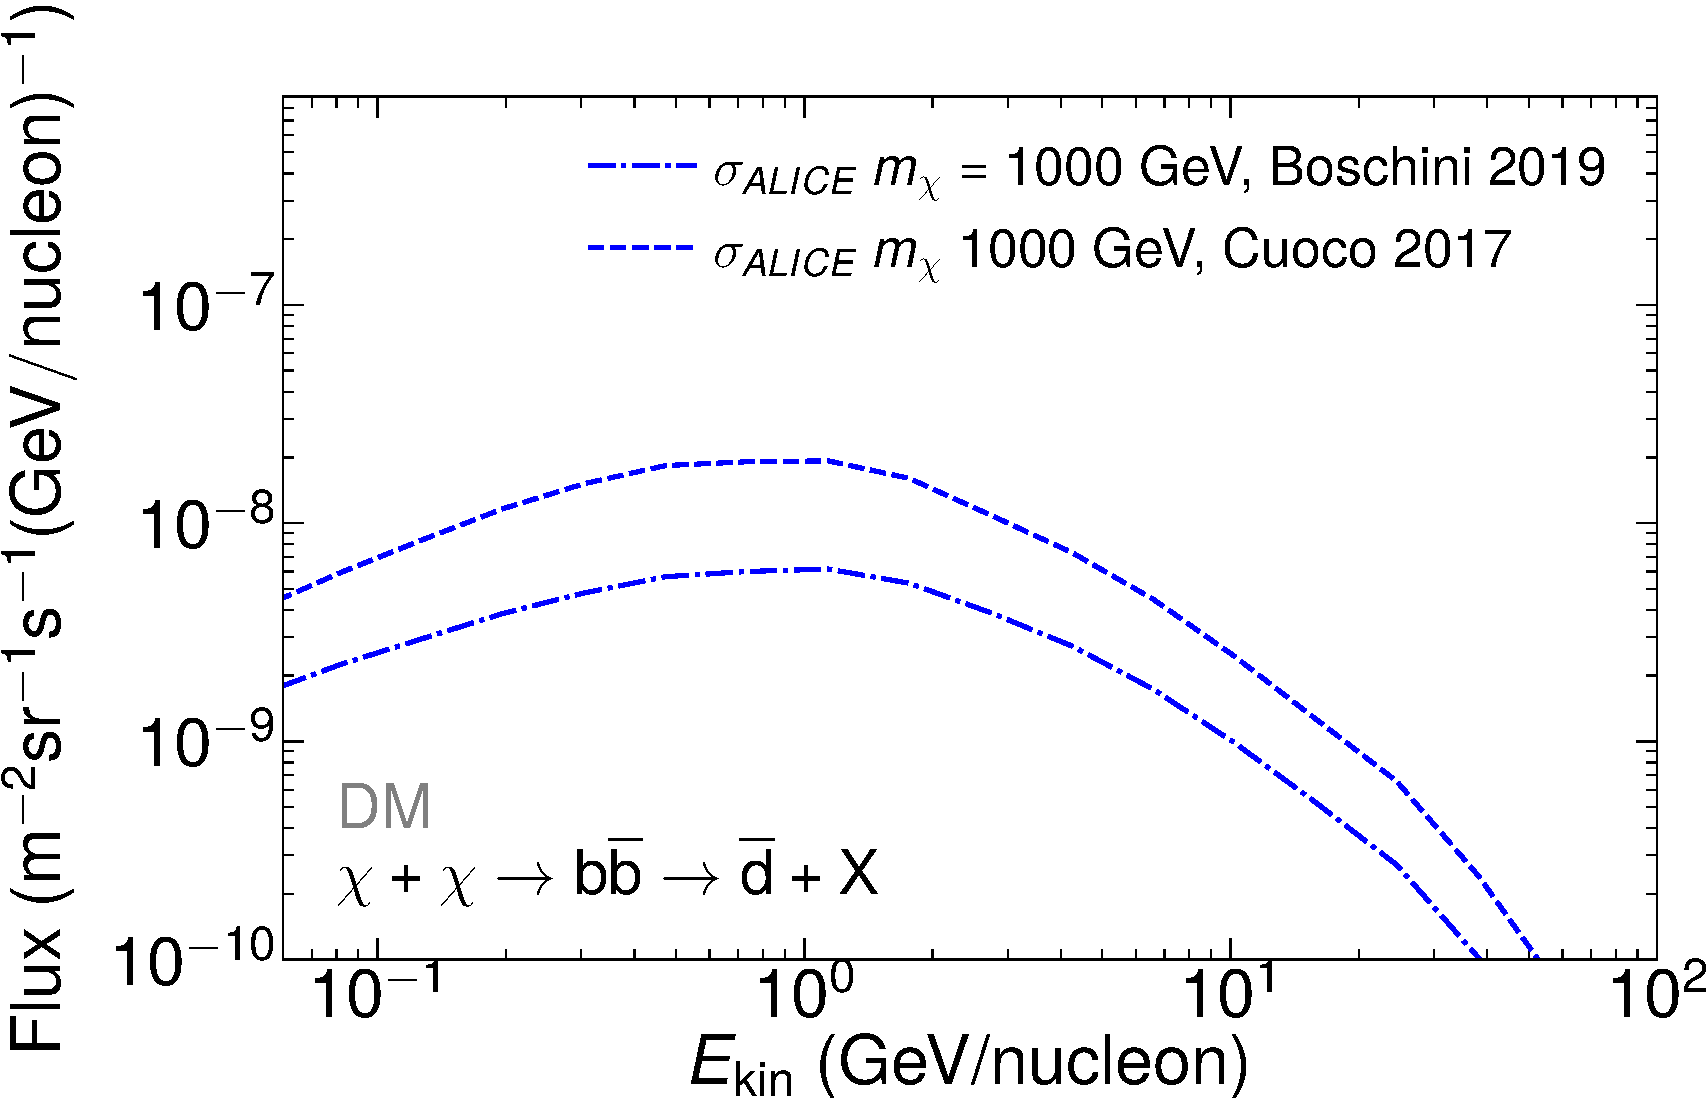
\includegraphics[width=0.48\textwidth]{figures/ComparisonPropagationBoschiniDM.pdf}
    \caption{Comparison between the different GALPROP propagation parameters used in this work, for antideuterons from high energy cosmic ray collisions (left) and from dark matter annihilations (right).}
    \label{fig:ComparisonPropagation}
\end{figure}

At this point it is also important to note the composition of both cosmic rays and the interstellar medium. For the interstellar medium, its composition determines the targets for incoming cosmic rays. This is important both for the production of secondary antinuclei in high energy cosmic ray collisions, and also for the annihilation of antinuclei as they travel through our galaxy. Both the interstellar medium and baryonic cosmic rays share similar compositions: 90\% protons and 9\% $^4\mathrm{He}$ \cite{}. The remaining elements is made up of heavier elements. 
\subsection{The Galprop framework}\label{sec:GALPROP}
The technical details of the implementation of antinuclei propagation in GALPROP can be found in \cite{ALICE-PUBLIC-2022-002}. The following section aims to give the reader an understanding of the concepts considered.\\

As already discussed in section \ref{sec:Propagation}, the Galprop framework functions by solving the transport equation numerically (equation \ref{eq:TransportEquation}). It does so by finding a steady state solution, iterating in smaller and smaller timesteps until a stable solution is found. During each timestep, it iterates over a position and momentum grid, the former of which can either be expressed in 2 dimensions (r and z) or 3 (x, y, z). Since we assume axial symmetry, the two are mathematically equivalent, so for the purpose of this work, the 2 dimensional method was chosen. \\

Galprop is configured by passing a set of parameters from an external text file. The important parameters are shown in table \ref{tab:GalpropParameters}. Of particular note are the Galaxy half height z$_h$, and the diffusion parameter D$_{xx}$, since these two are degenerate for cosmic rays from non-exotic sources. The actual parameter which is being fixed is the ratio of the two. This is because for non-exotic sources, the number of sources doesn't change so any change in position is compensated by increased diffusion. For a dark matter source however, the height of the galaxy has direct implications for the number of dark matter sources, so this degeneracy is broken.\\


\begin{table}[h]
    \centering
    \begin{tabular}{|c|c|c|c|}
        \hline
        Parameter &  Units & Best fit value from Boscini & Best Fit value from Cuoco \\
        \hline
        z$_h$  & kpc &  4 & 6.78 \\
        \hline
        D$_{xx}$ & cm$^2$s$^{-1}$& 4.5 \times $10^{28}$ & 7.48 \times $10^{28}$ \\
        \hline
    \end{tabular}
    \caption{Two of the parameters for the tuning of Galprop, which show the degeneracy between them.}
    \label{tab:GalpropParameters}
\end{table}

It is important to note that the main parameter which affects a lot of propagation is the so called grammage, which is the amount of matter of the interstellar medium which particles have to traverse. This is the product of the density of the interstellar medium and the path length of the particles, and can be constrained by the ratio of primary to secondary cosmic rays, according to equation \ref{eq:B_to_C_eq}\footnote{This is the simplified equation without losses, for more details see \cite{GALPROP_Expl_Supplement}, section 7.1.}
\begin{equation}
    \psi_s / \psi_p = \frac{n\Delta z \sigma \beta c z_h}{2D_{xx}}
    \label{eq:B_to_C_eq}
\end{equation}
, where $n$ is the density of matter in the interstellar medium, $\psi_p$ and $\psi_s$ are the primary and secondary fluxes, and $\sigma$ is the production cross section of the secondary particles when the primary cosmic rays interact with the interstellar medium. This means that this ratio is simply the amount of matter traversed $\times$ the production cross section $\times$ $\frac{z_h}{2D_{xx}}$, which shows the degeneracy for these parameters. The primary to secondary ratio is best constrained from the Boron-to-Carbon (B/C) ratio, since Carbon is expected to be produced mostly during stellar processes, while all Boron is produced in collisions of heavier nuclei with the ISM\cite{AMS_B_to_C}. This ratio has been measured by the AMS collaboration to very high accuracy\cite{AMS_B_to_C}, with errors less than 3\% up to rigidities of 100 GV.\\

Antinuclei are not by default included in Galprop. Fortunately, the framework is capable of handling negative nuclei with antiprotons, therefore the extension was done by providing the mass of the antideuteron/antihelium, their inelastic cross sections on the interstellar medium, and their source functions. Separate entries were used for the secondary production from high-energy cosmic rays and from dark matter annihilations. The inelastic cross section had to be provided on a proton and helium target, which are significantly lighter than the average detector materials probed in the measurements shown in section \ref{sec:ResHe3SigmaInel}, therefore the results had to be extrapolated to these lighter targets. The exact methods of the extrapolations are explained in section \ref{sec:ResAnnInOurGalaxy}.\\

The source functions for antinuclei from either high-energy cosmic-ray collisions or from dark matter annihilations were included in GALPROP as a function of the distance from the galactic centre. For the dark matter part, this can be done simply by evaluating equation \ref{eq:DM_source_term} described above for a specific radius and kinetic energy. However, for antinuclei from high-energy cosmic rays this is not possible, since the spectrum of cosmic rays at a given point enters into the equation. Therefore, the production cross sections for the relevant collision systems (pp, p--He, He--p, He--He) were implemented in GALPROP, and the interactions between those cosmic-ray species were calculated as described in \cite{ALICE-PUBLIC-2022-001}, based on the production cross sections in \cite{}. 

\subsection{Annihilations within our galaxy}\label{sec:ResAnnInOurGalaxy}
As antinuclei travel through our galaxy, they might inelastically interact with matter in the interstellar medium. This can either be in the form of inelastic scattering\footnote{Non-annihilating inelastic scattering of antinuclei on matter is expected to be very rare. An example of this would be the collision of \ahe\ with a $^4\mathrm{He}$ nucleus which causes the $^4\mathrm{He}$ nucleus to break up, and thus a drastically different momentum for the \ahe\ . Since such particles would be lost to the tracking algorithm in the ALICE detector, these processes are included in the measurements of the inelastic cross section. However, in the galaxy such particles would not disappear and thus could in theory be detected (this is usually called tertiary production). Since the expected flux caused by this effect is several orders of magnitude lower than a signal, it is neglected for the purposes of this thesis.} or annihilation, although of the two the latter is expected to be dominant \cite{}. The result of these interaction is thus mostly the disappearance of the antinuclei. The produced particles are mostly pions, and thus not stable enough to detect them and maybe extract a signal from them. Some high-energy photons could also be produced, and such gamma rays are the target of specific sky surveys looking for large areas of antimatter, which when coming into contact with matter should produce a detectable signal. However, a single annihilation would be undetectable at any significant distance. We can therefore conclude that the relevant result of annihilation is the disappearance of the antinucleus in question. \\

The loss of antinuclei in Galprop was taken into account by implementing the inelastic cross section. As antinuclei are propagated throughout our galaxy, the total amount of matter they interact with is calculated for each timestep, position and momentum grid point (see section \ref{sec:GALPROP} for details). In order to do so, both the distribution and the composition of the interstellar medium is required. The composition is known to a relatively high accuracy \cite{}, and is dominated by hydrogen, which makes up $\approx$90\% of the total mass in the interstellar medium. The remainder is mainly helium, making up $\approx 9\%$ of the total mass. During each calculation step, the inelastic cross sections on the dominant species of the interstellar medium (hydrogen and helium) are used to calculate how many antinuclei are lost in each momentum bin. Therefore, it is necessary to evaluate the cross sections on these very light targets, rather than the heavy targets on which they were measured.\\

In order to extrapolate the results of the inelastic cross sections to light targets, the A scaling from Geant was applied. To achieve this, the deviation of the inelastic cross section from the default implemented in Geant was obtained for the mean material in ALICE, as described in section \ref{sec:ResHe3SigmaInel}, and proportianlly applied to the antinucleus-proton cross section in Geant. This assumes that the relative scaling is the same regardless of the target nucleus, and an additional 8\% uncertainty is assigned to allow for any deviation from this assumption. This value was achieved by comparing the $A$ scaling used in Geant4 and in full Glauber calculations\cite{antiHe3XS, glauber_model_geant4_scaling}. For values outside the range of the measurements detailed in sections \ref{sec:ResHe3SigmaInel}, the scaling factor at the last available momentum was used.
The resulting cross sections are shown for both antideuterons and \ahe\ in figure \ref{fig:ScaledXS_ahe_adeut}. The Geant lines shown in these figures are based on Glauber model calculations, as discussed in section \ref{sec:IntroGlauber}.

\begin{figure}[hbtp]
    \centering
    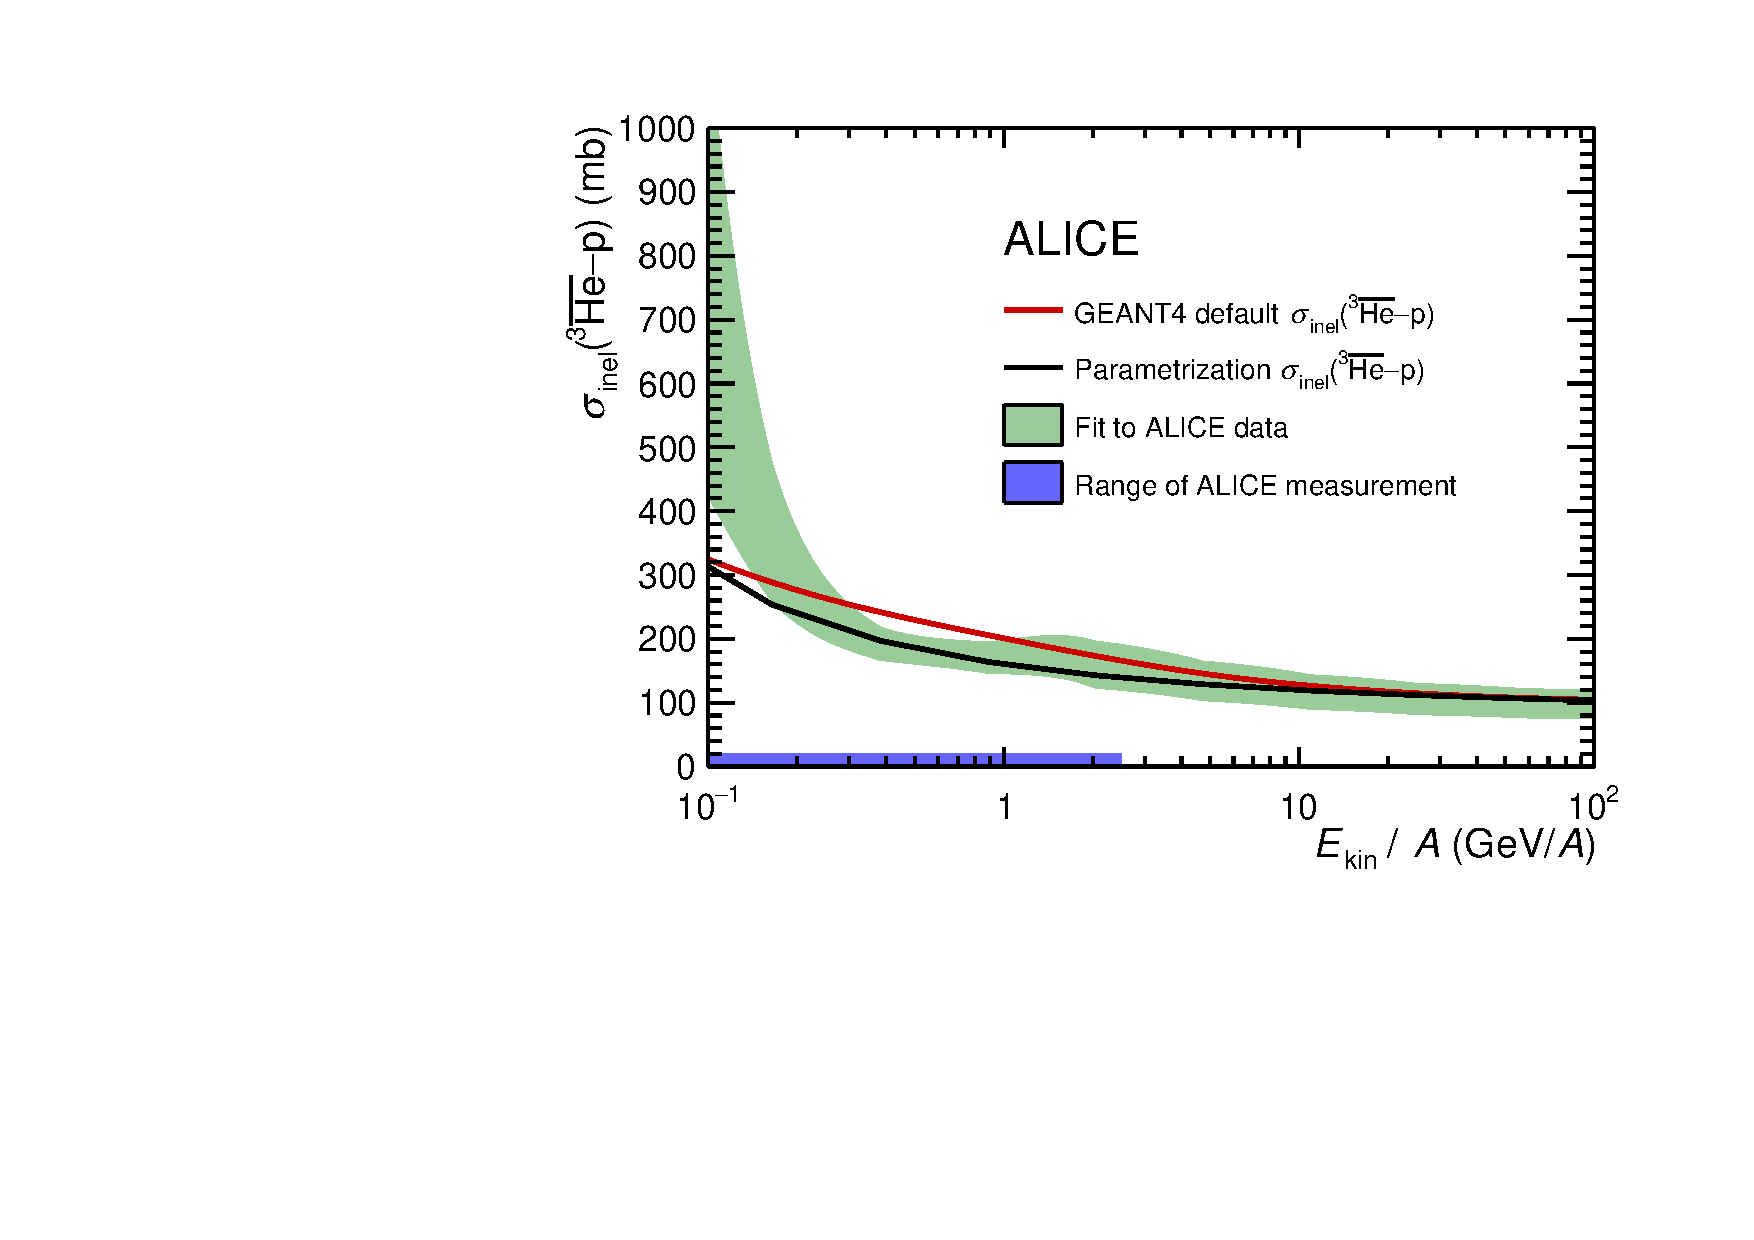
\includegraphics[width=0.45\textwidth]{figures/Antihelum_on_p_targets_scaled_with_paramterisation.pdf}
    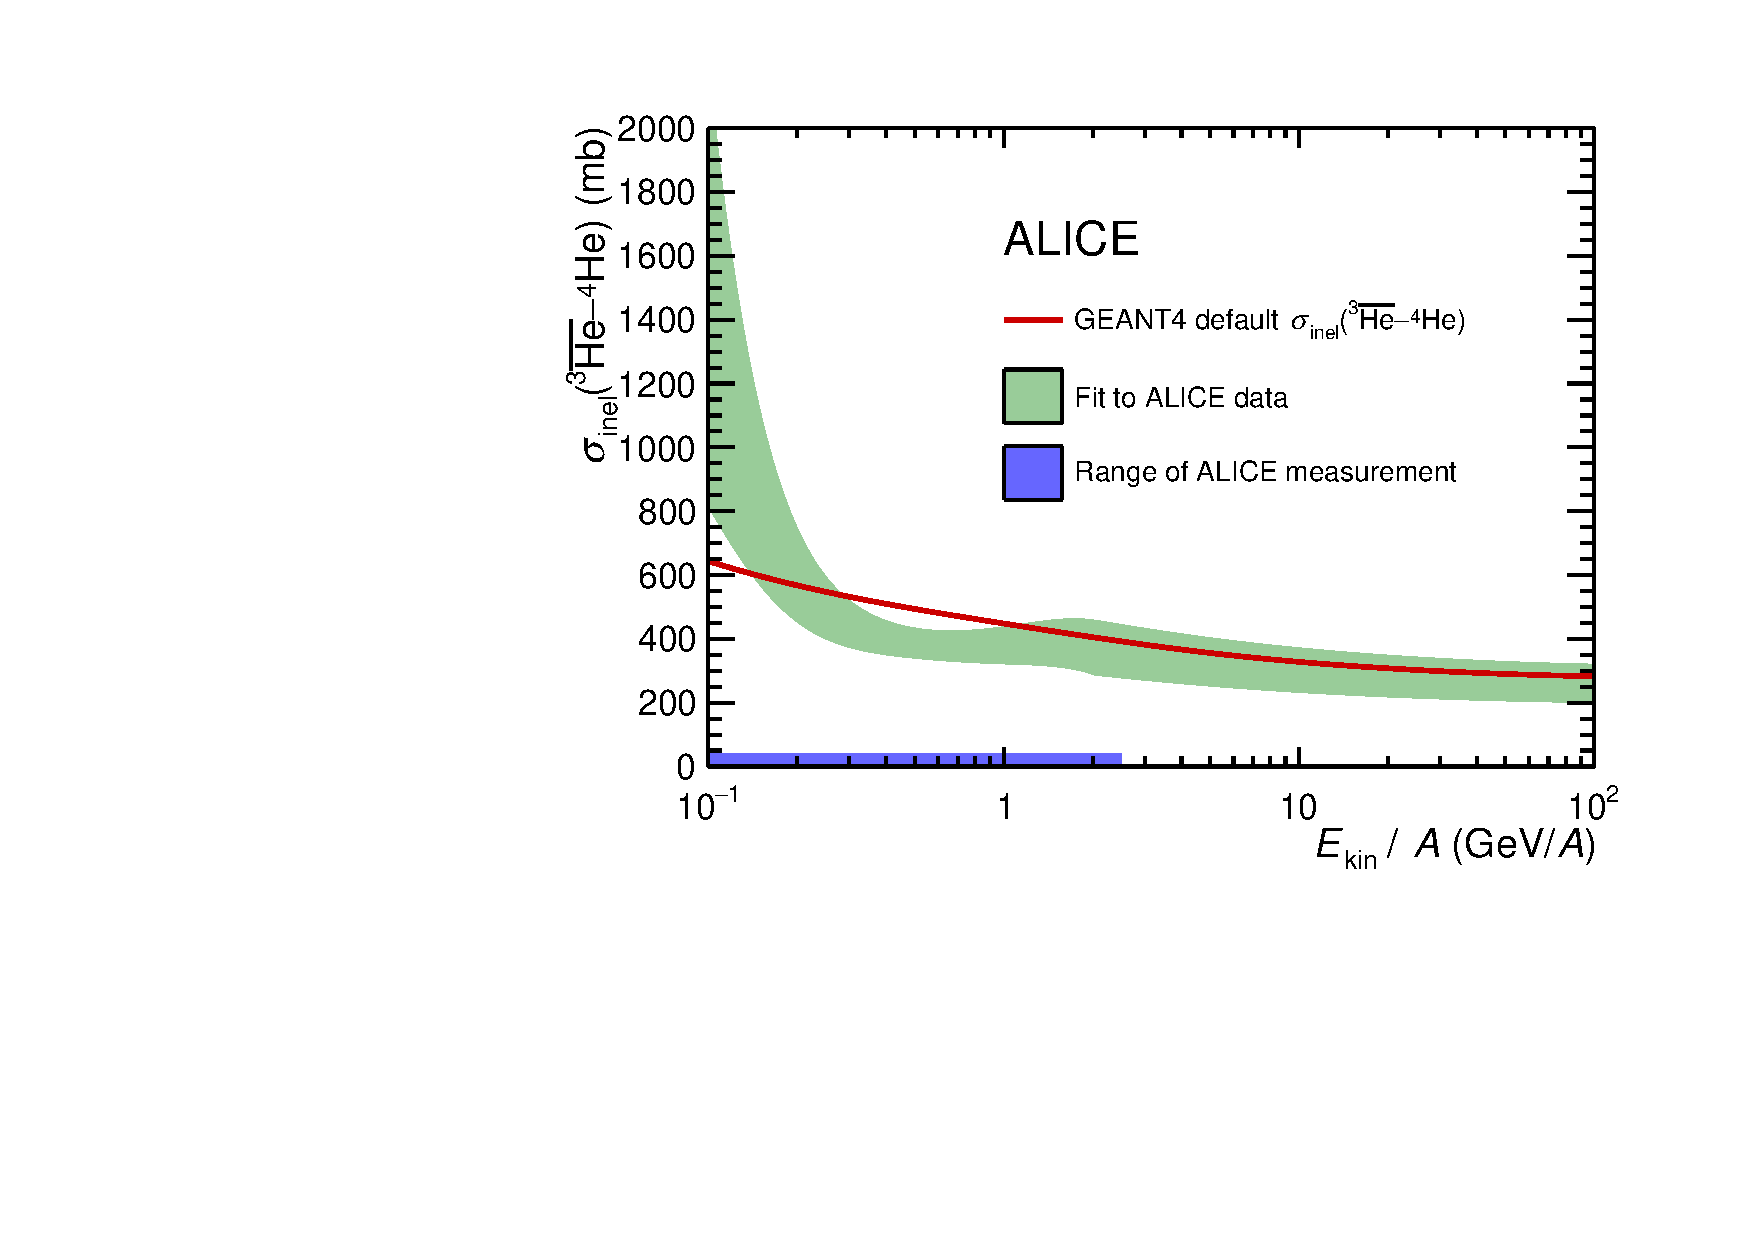
\includegraphics[width=0.45\textwidth]{figures/Antihelum_on_p_targets_scaled.pdf}
    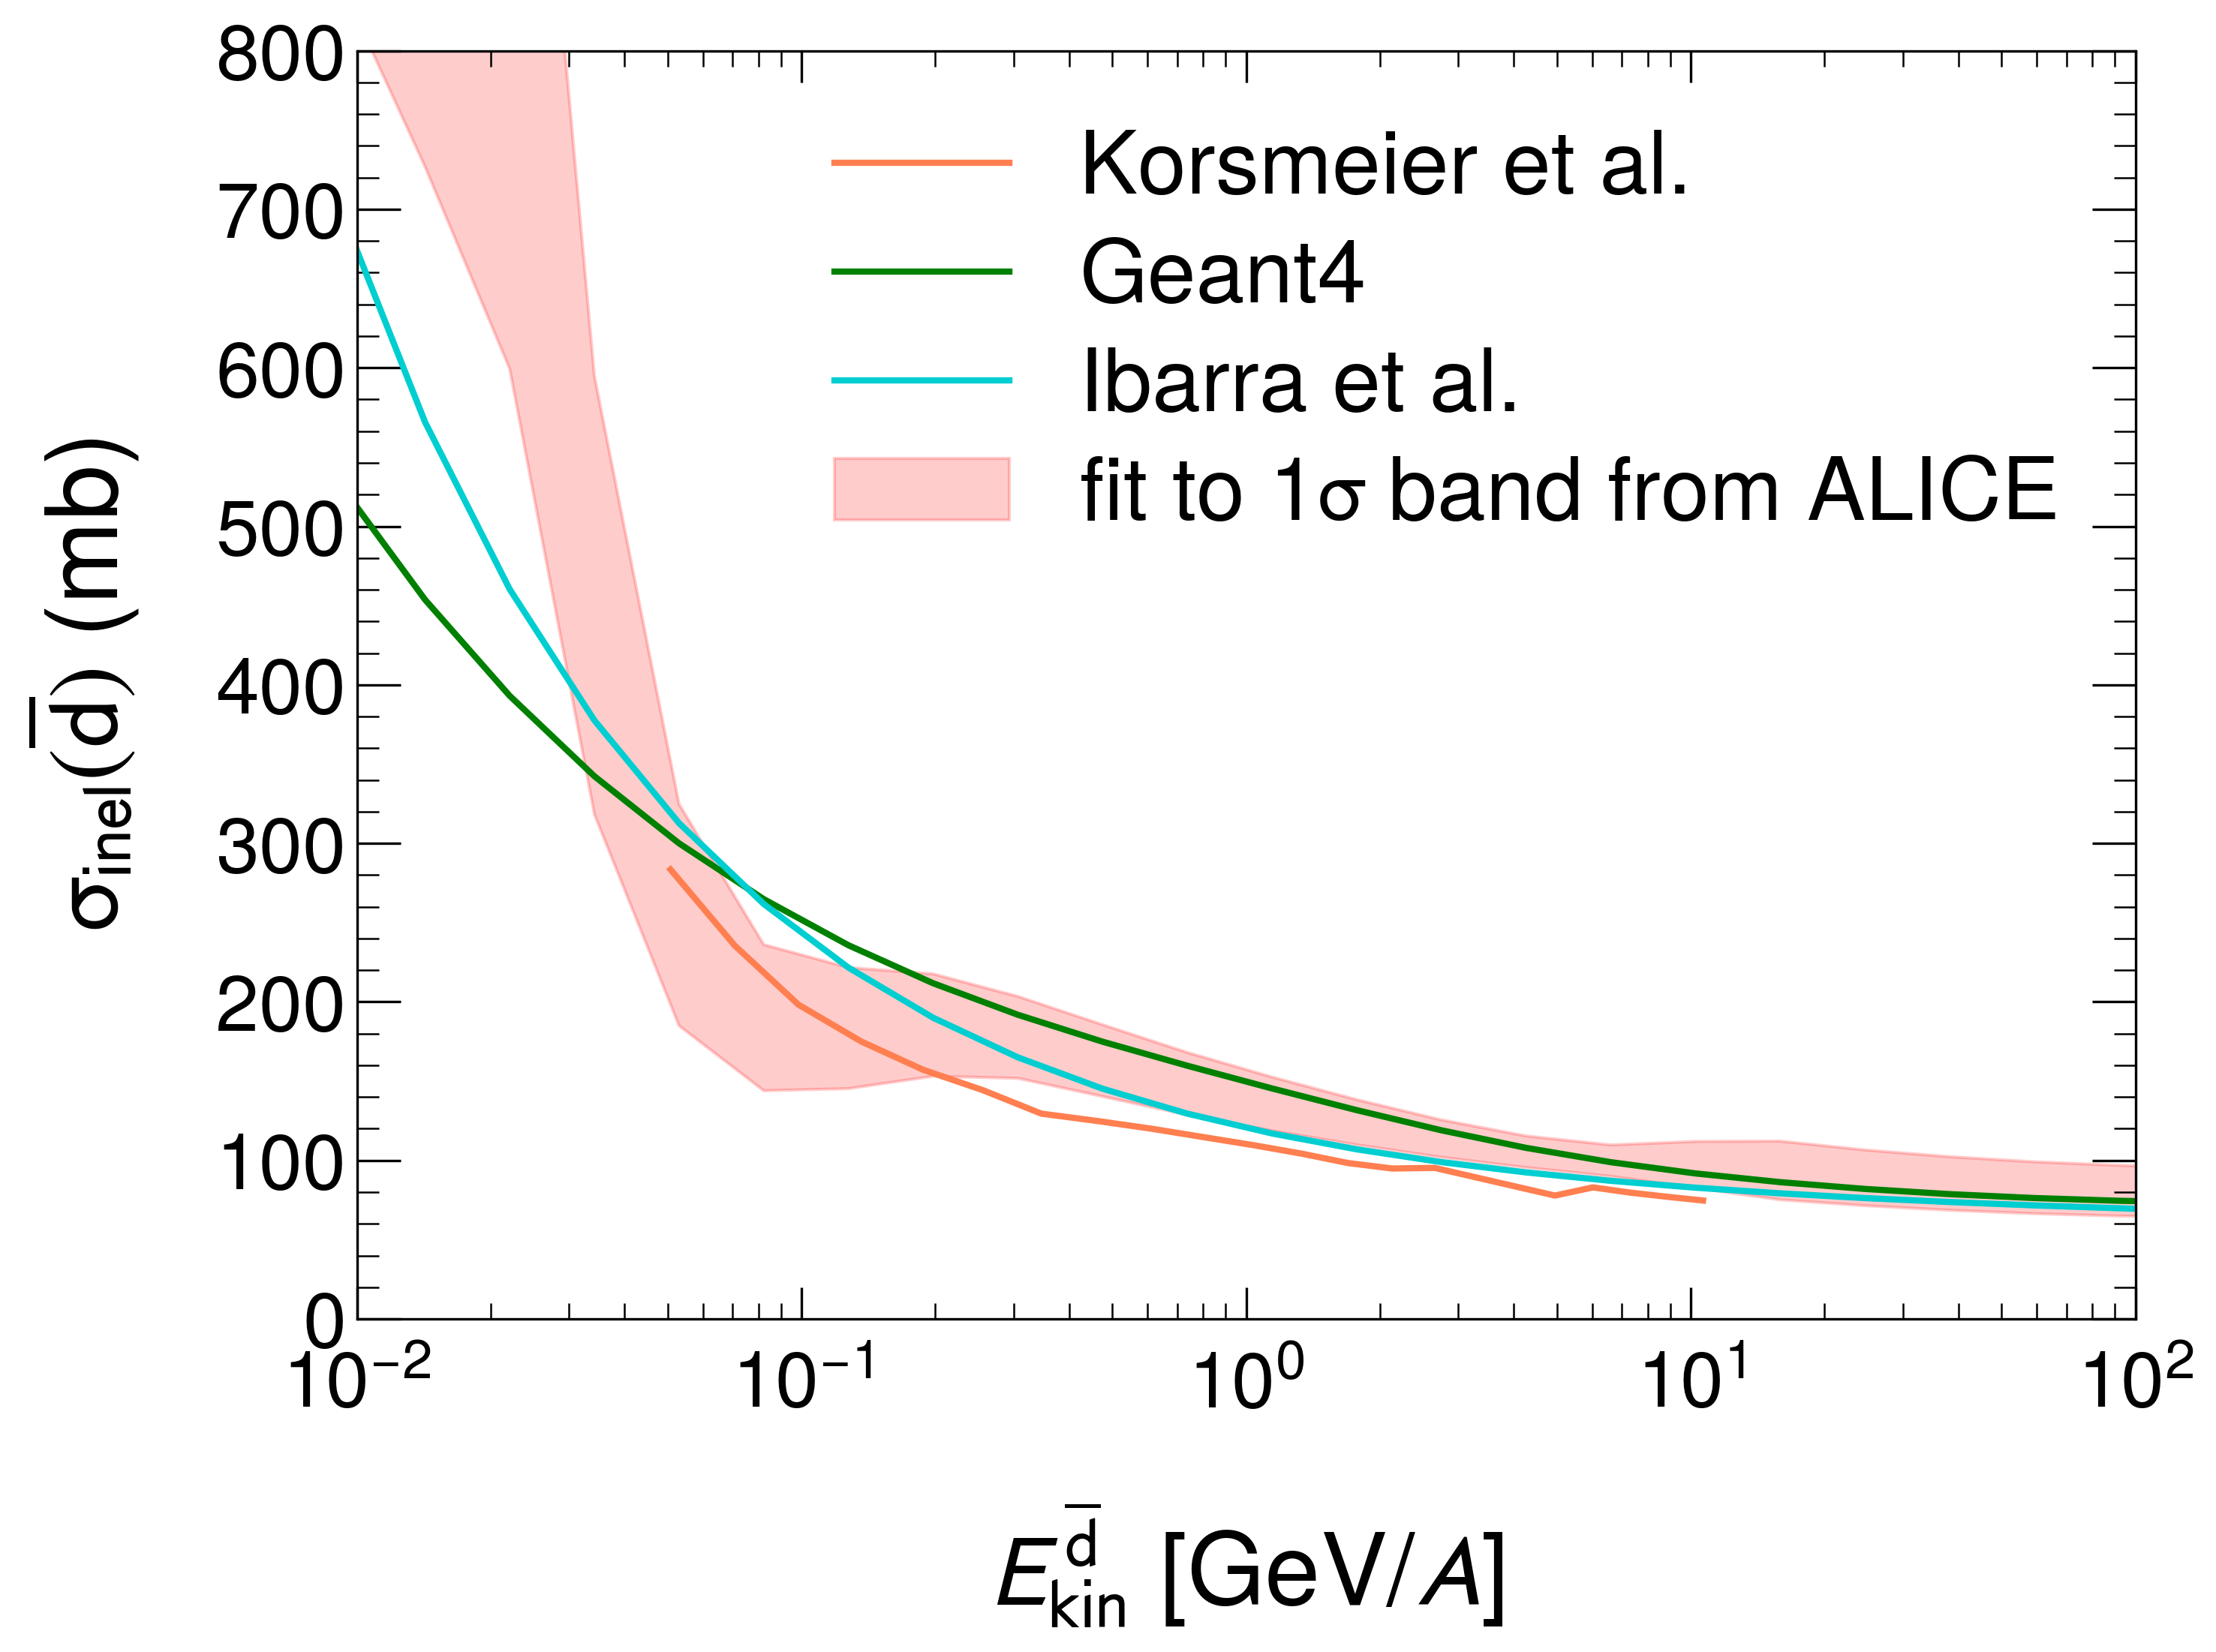
\includegraphics[width=0.45\textwidth]{figures/dbar_xs_comparison_dbarNotInLabels.png}
    \caption{Scaled inelastic cross sections of \ahe\ (top) on proton (left) and Helium-4 (right) targets and antideuterons on proton targets (bottom). The band shows the experimental uncertainty from the ALICE measurements \cite{}, plus an additional 8\% uncertainty associated with the scaling from heavier targets (C, O, Al) to protons (H). The parameterization shown in the top left panel (labeled Korsmeier et al in the bottom panel) is taken from \cite{Korsmeier2018}, and is based on scaling the total deuteron-antiproton cross section by the inelastic portion of the antiproton-proton cross section, and then scaling the obtained value by 3/2 to account for the extra nucleon in \ahe\. The cross section in the bottom panel labeled Ibarra et. al. is taken from \cite{Ibarra:2012cc}, and is based on taken 2 times the antiproton-proton inelastic cross section, as parameterized by \cite{Ibarra2012cc_ref40}. See section \ref{sec:IntroGlauber} for a more detailed discussion on calculating inelastic cross sections.}
    \label{fig:ScaledXS_ahe_adeut}
\end{figure}

\subsection{Antinuclei fluxes for different dark matter masses and annihilation channels}
In this section the effects of different dark matter masses on antinuclei fluxes will be discussed. The fluxes are compared to a prediction for secondary antinuclei from high-energy cosmic ray collisions with the interstellar medium. In the lower panel on figure \ref{fig:Results_He3_fluxes_diff_DM_masses} and  on the right side of figure \ref{fig:different_DM_profiles_and_transparencies}, the transparency of the galaxy to antinuclei is shown. This is defined in equation \ref{eq:TransparencyDefinition} as the ratio of the obtained flux with a given non-zero inelastic cross section, to the flux obtained when all inelastic interactions are turned off. The dark matter self annihilation cross section used for the dark matter models shown in this chapter is $<\sigma v>=2.7 \times 10^{-26}$cm$^3 \mathrm{s}^-1$, unless otherwhise noted. This is compatible with the currently allowed limit, and also at the thermal value of the cross section, which is discussed in section \ref{sec:WIMPS}. 

\begin{equation}\label{eq:TransparencyDefinition}
    \mathrm{Transparency(\sigma_{inel})} = \frac{\mathrm{Flux(\sigma_{inel}})}{\mathrm{Flux(\sigma_{inel}=0})} 
\end{equation}

Several parameterizations of the inelastic cross sections were considered and are shown for the fluxes in this section. The colored bands represent the results obtained using the inelastic cross sections measured by ALICE, and the associated experimental uncertainties from this measurement. The solid lines denote the results obtained using the default inelastic cross sections implemented in Geant4. 
% shouldn't one add a short paragraph discussing various sigma_inel used in the plots? Describe that the lines are the results using sigma_inel from Geant4 and "bands" (with very small uncertainty of 10-15%) are from ALICE measurements of sigma_inel(antid). The uncertainties on the fluxes due to inelastic interactions are small, and this result is also part of your thesis, highlight it!

\subsubsection{Results for antideuterons}
The antideuteron fluxes inside and outside of the solar system can be seen in figure \ref{fig:Results_dbar_fluxes_diff_DM_masses}. Of particular note is the signal to background ratio, i.e. the ratio between secondaries coming from cosmic-ray collisions and fluxes from dark matter. At low energies, for values of $m_\chi \lesssim 100$ GeV , the signal exceeds the secondaries by several orders of magnitude at energies energies below ca.\ 3 GeV/A. This reinforces low-energy antideuterons as a unique probe for indirect dark matter searches. At larger energies the spectral shape of the antideuteron fluxes from dark matter becomes very similar to the one expected for secondaries, and also the normalisation becomes very similar. This makes WIMP models with masses above ca. 1 TeV difficult to differentiate from secondary production, and thus loses the strength for probing such dark matter models. \\
The largest flux is achieved by the 10 GeV dark matter mass model, which is due to the increased normalisation due to the $1/m_\chi$ term. However, for such low dark matter masses, the used dark matter self annihilation cross section has been ruled out by antiproton limits, as can be seen in figure \ref{fig:DMSigmaVLimits}. Thus, the flux at 51 GeV would produce the largest allowed antideuteron flux. \\

For antideuterons, and additional channel was considered in addition to the usual \WW\ and \bb\ channels: a boosted production via the intermediate production of $\overline{\Lambda_b}$ and its subsequent decay, as described in \cite{}. This particular channel was only recently considered, and is expected to boost antinuclei yields. The validity of the approach rests on the fact that normal tunes of event generators under represent both the production of $\overline{\Lambda_b}$ and its branching fraction into antinuclei, however, this needs to be followed up with measurement to clearly determine the actualy size of this effect. \\
There are also two different background models considered for antideuterons, labeled Shukla et. al. based on \cite{}, and Kachelriess et al. based on \cite{}. For more details see \cite{}.

\begin{figure}[hbtp]
    \centering
    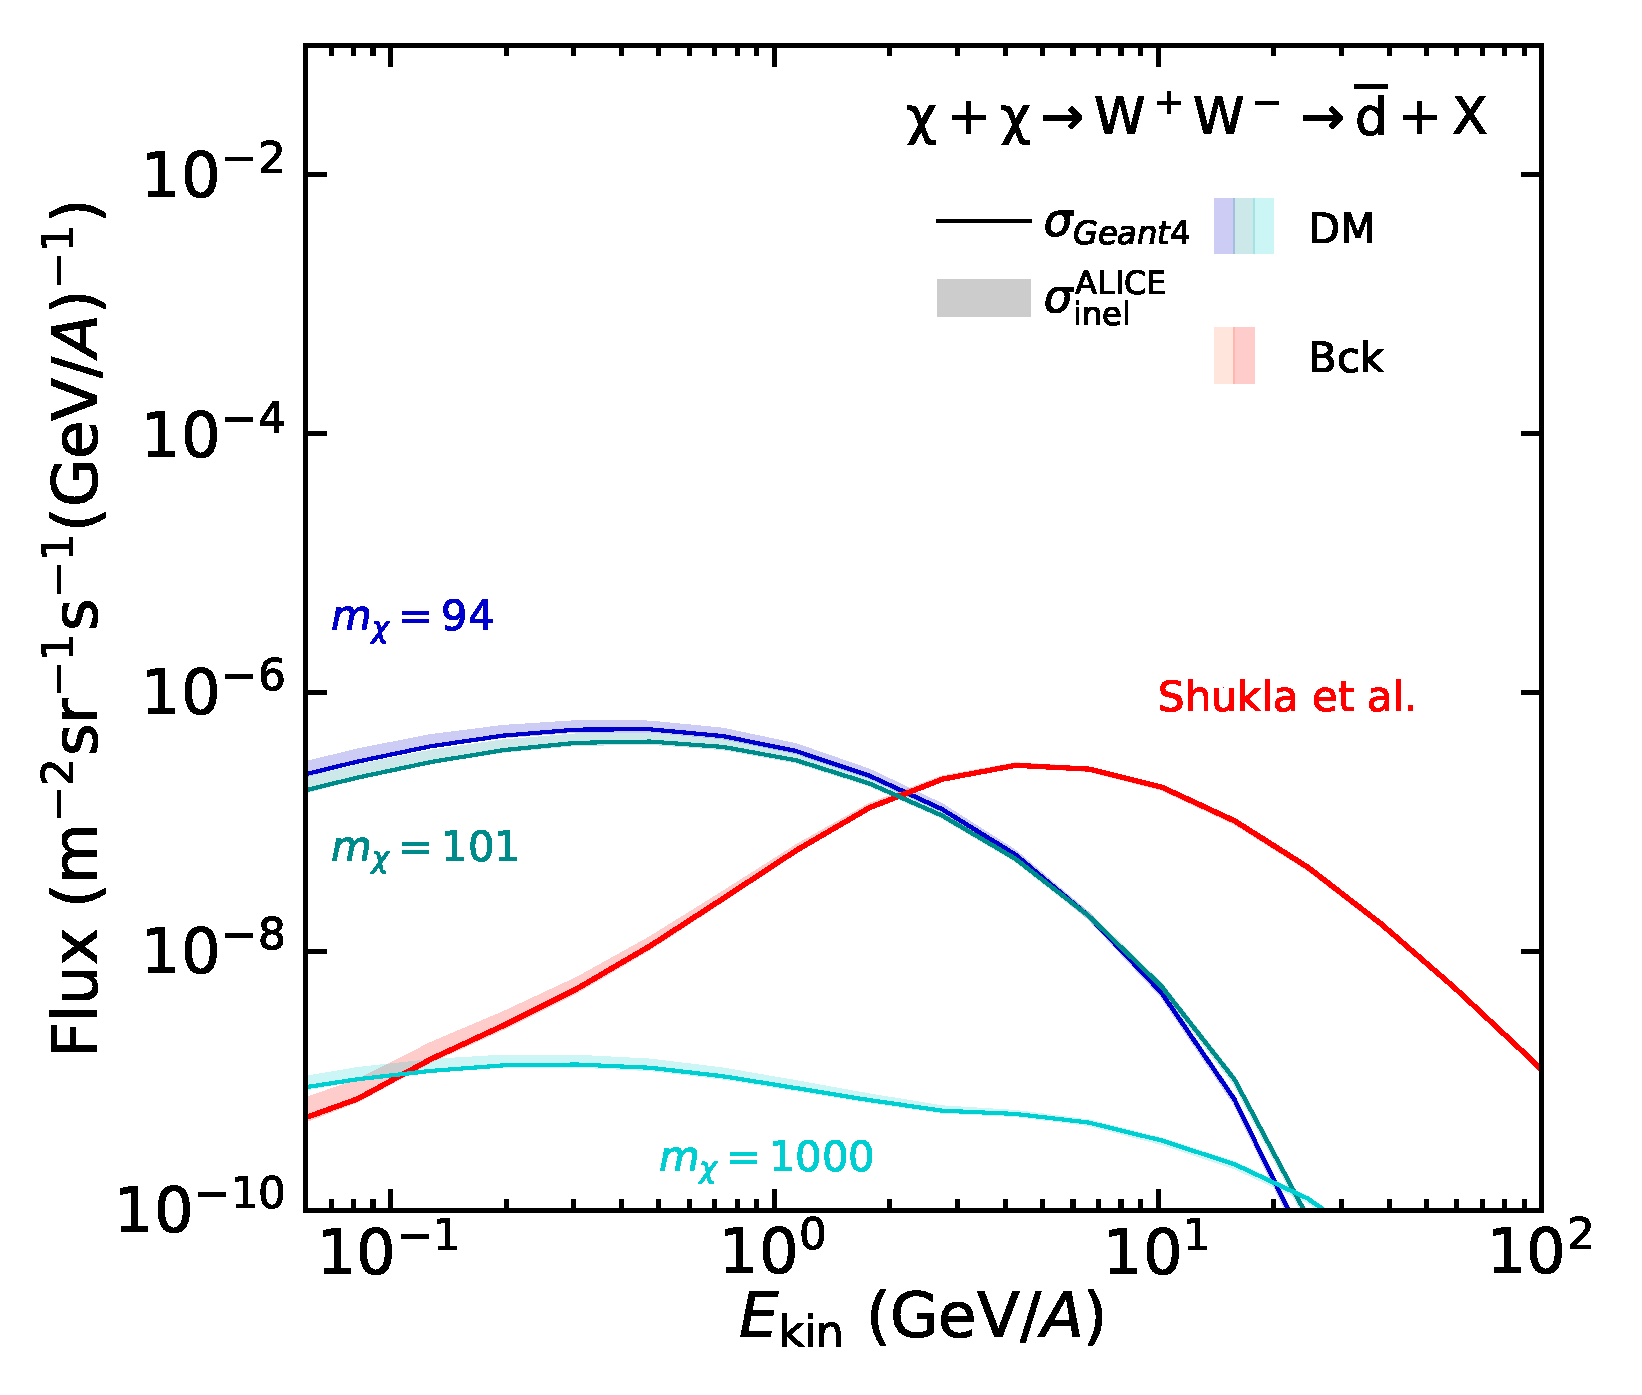
\includegraphics[width=0.49\textwidth]{figures/antideuteron_LIS_WW.pdf}
    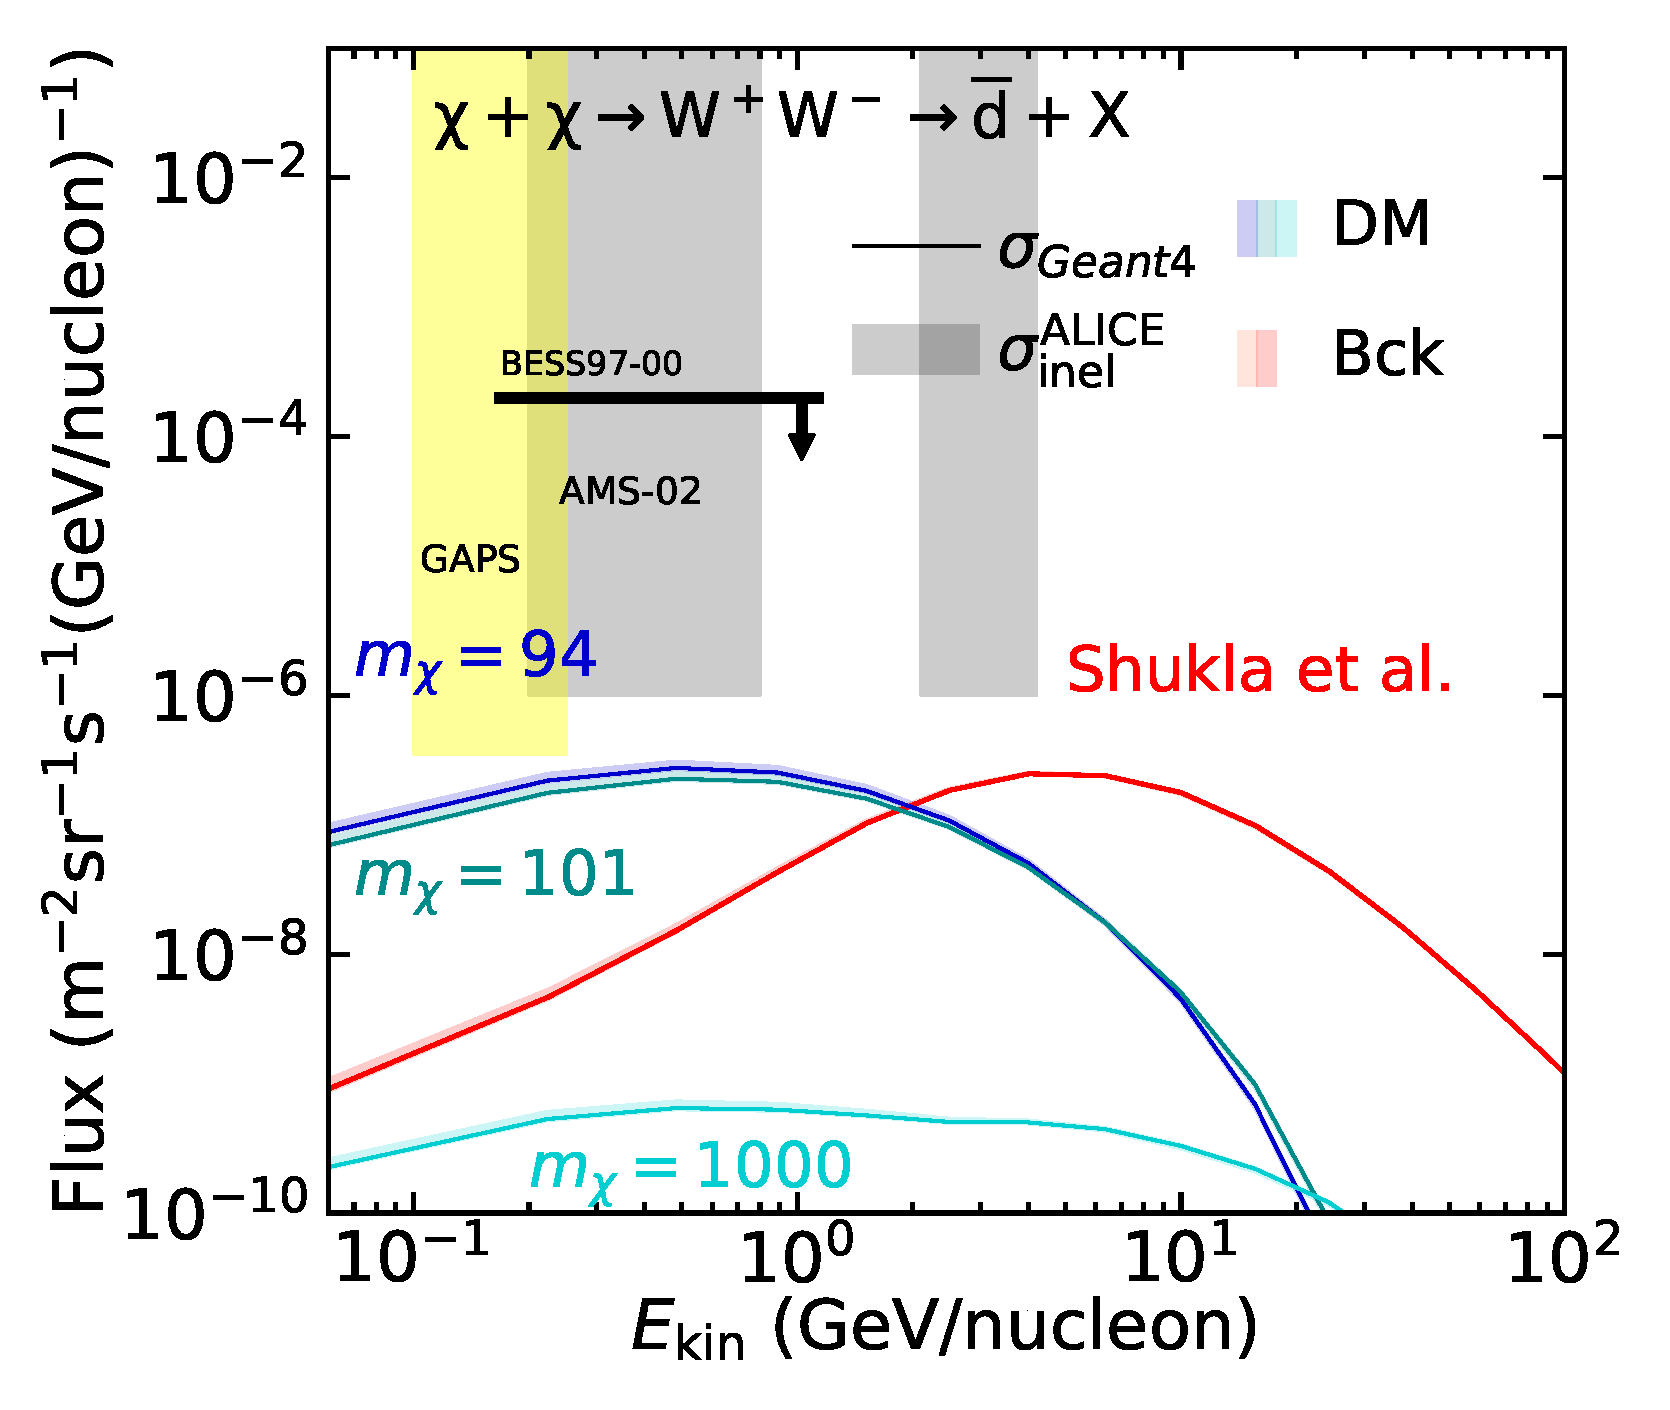
\includegraphics[width=0.49\textwidth]{figures/antideuteron_TOA_WW.pdf}
    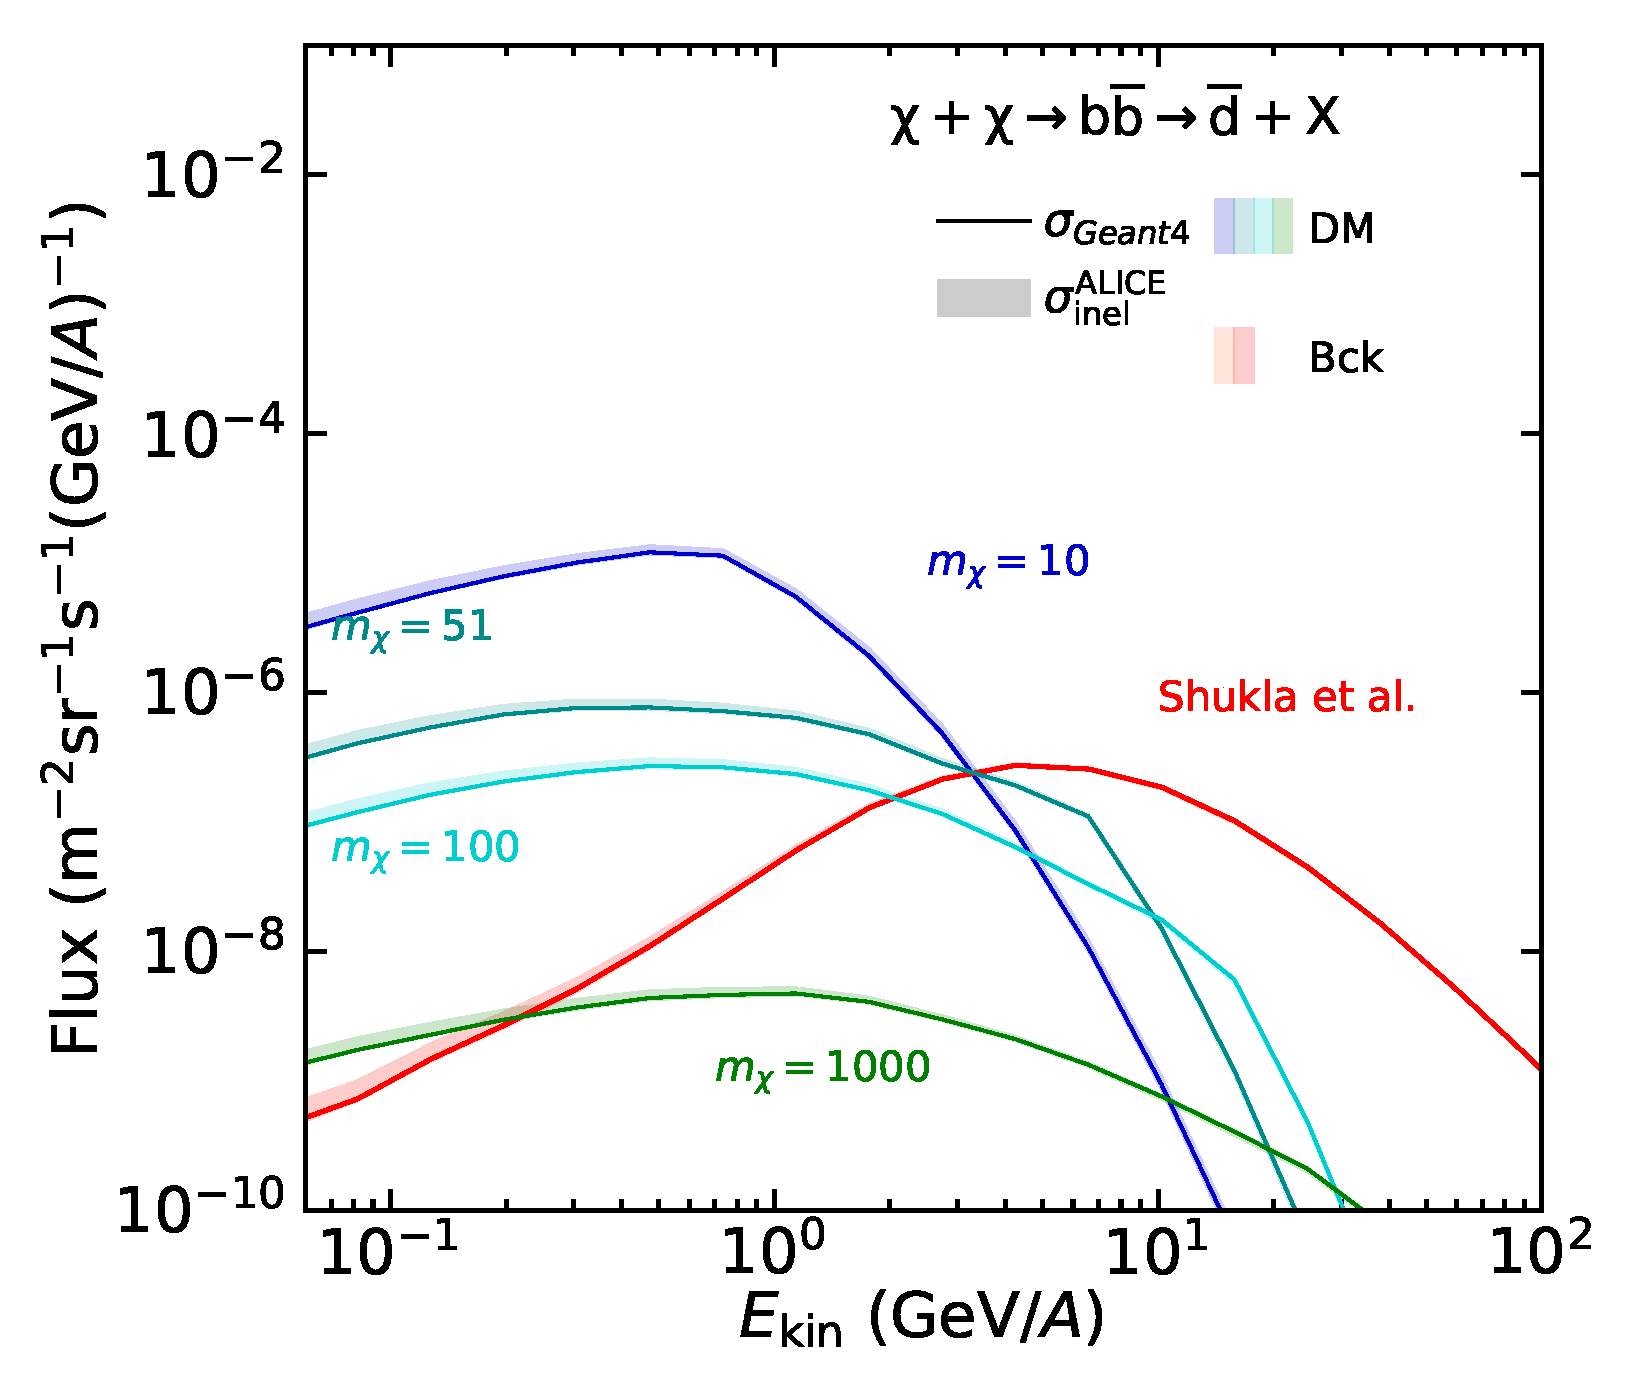
\includegraphics[width=0.49\textwidth]{figures/antideuteron_LIS_bb.pdf}
    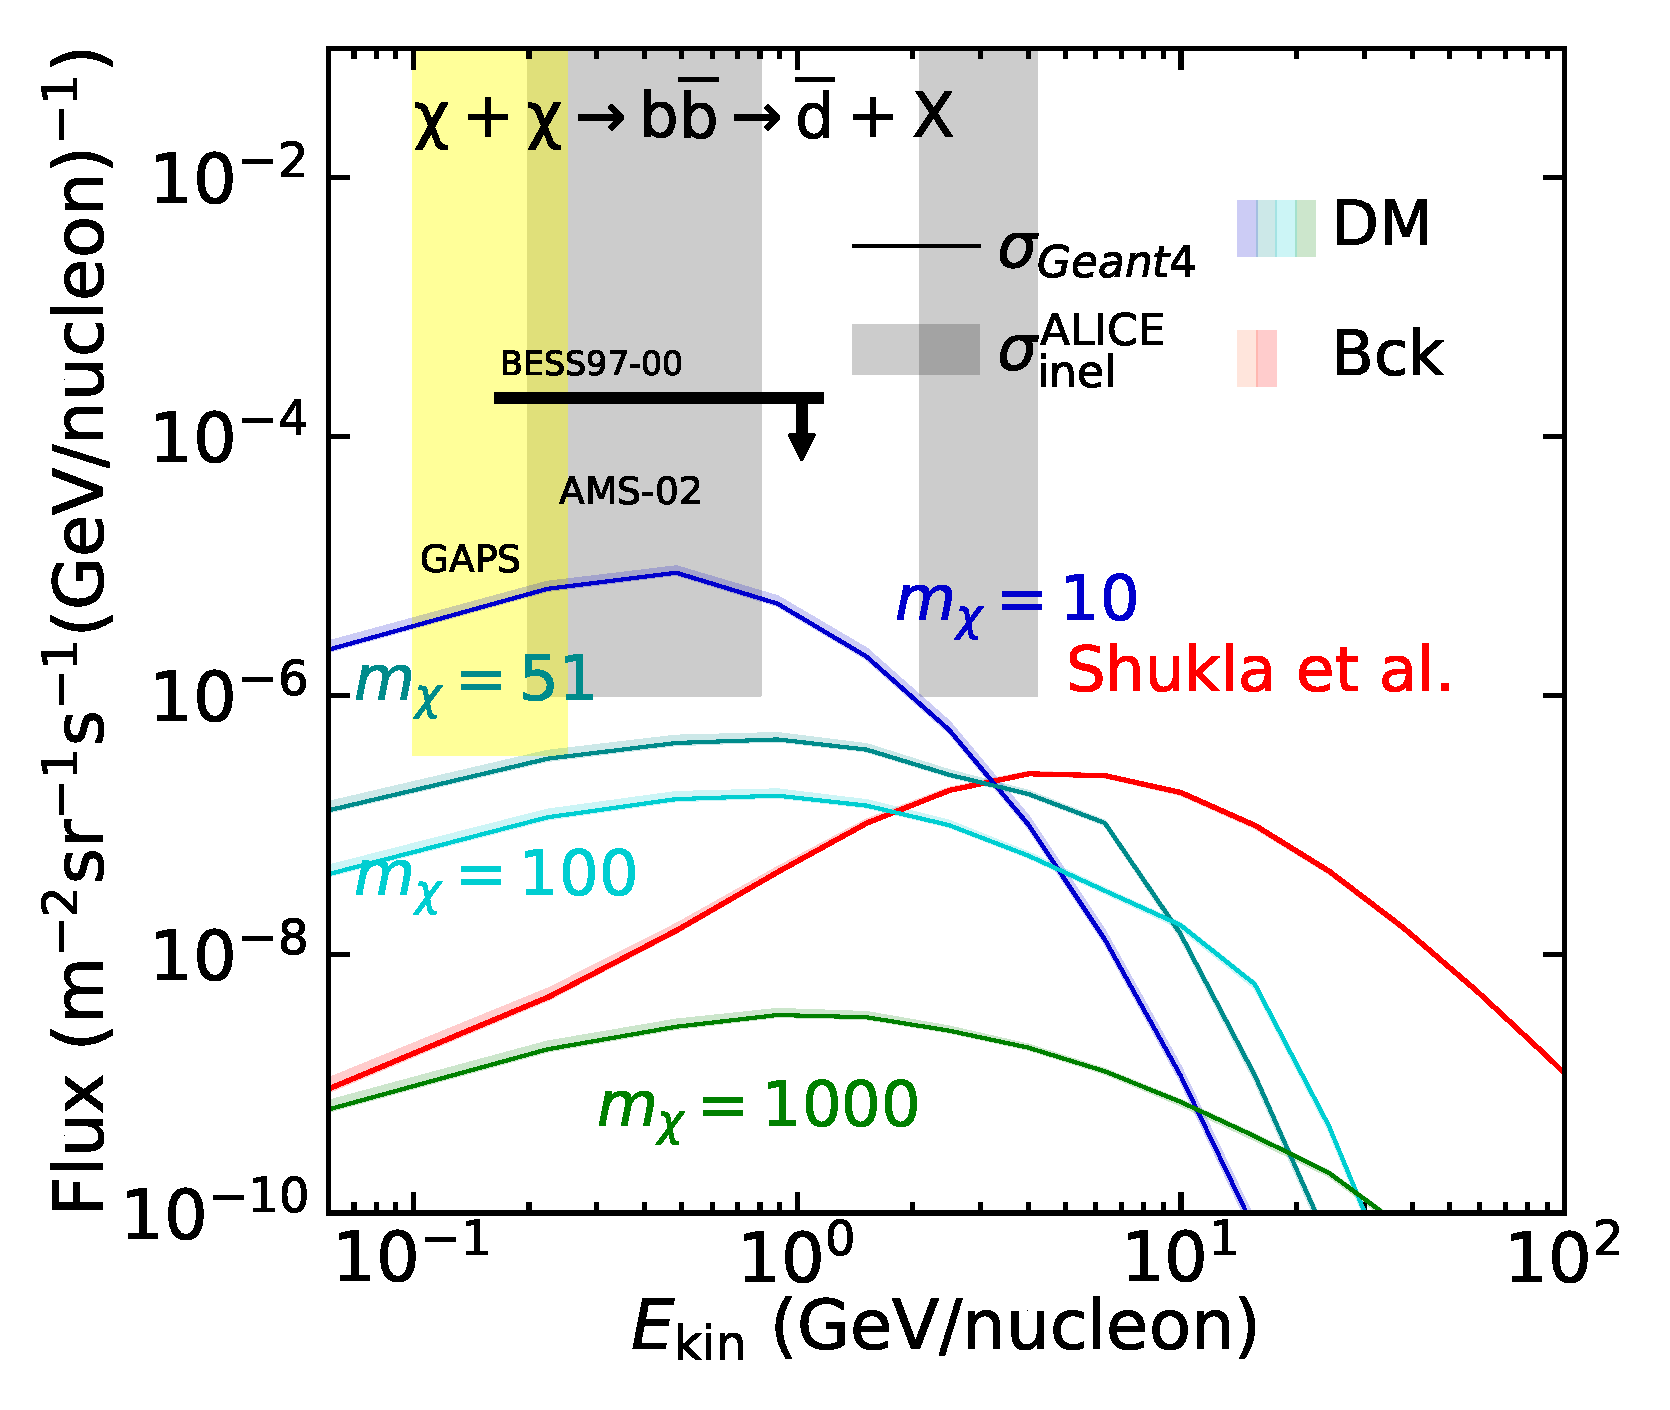
\includegraphics[width=0.49\textwidth]{figures/antideuteron_TOA_bb.pdf}
    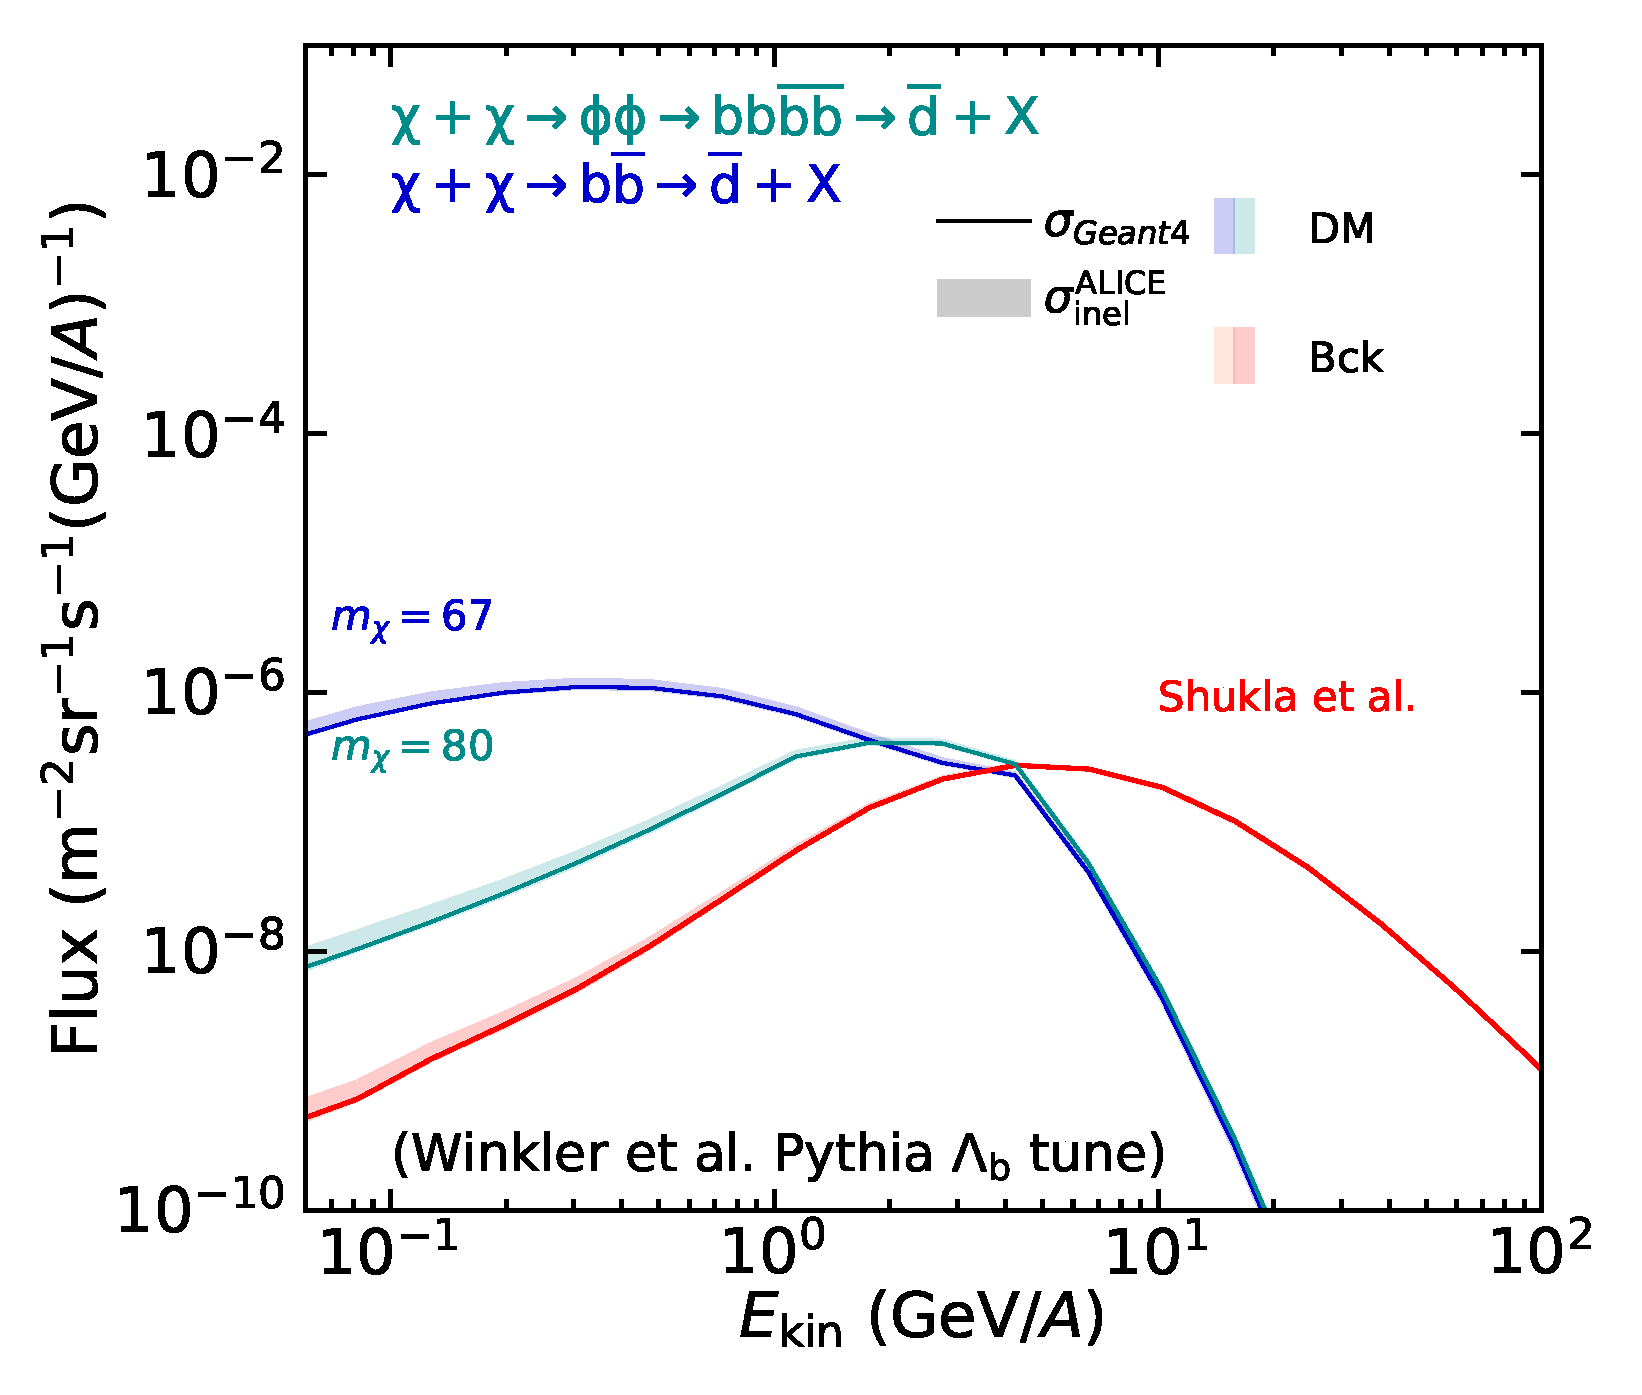
\includegraphics[width=0.49\textwidth]{figures/antideuteron_lambdaB_LIS.pdf}
    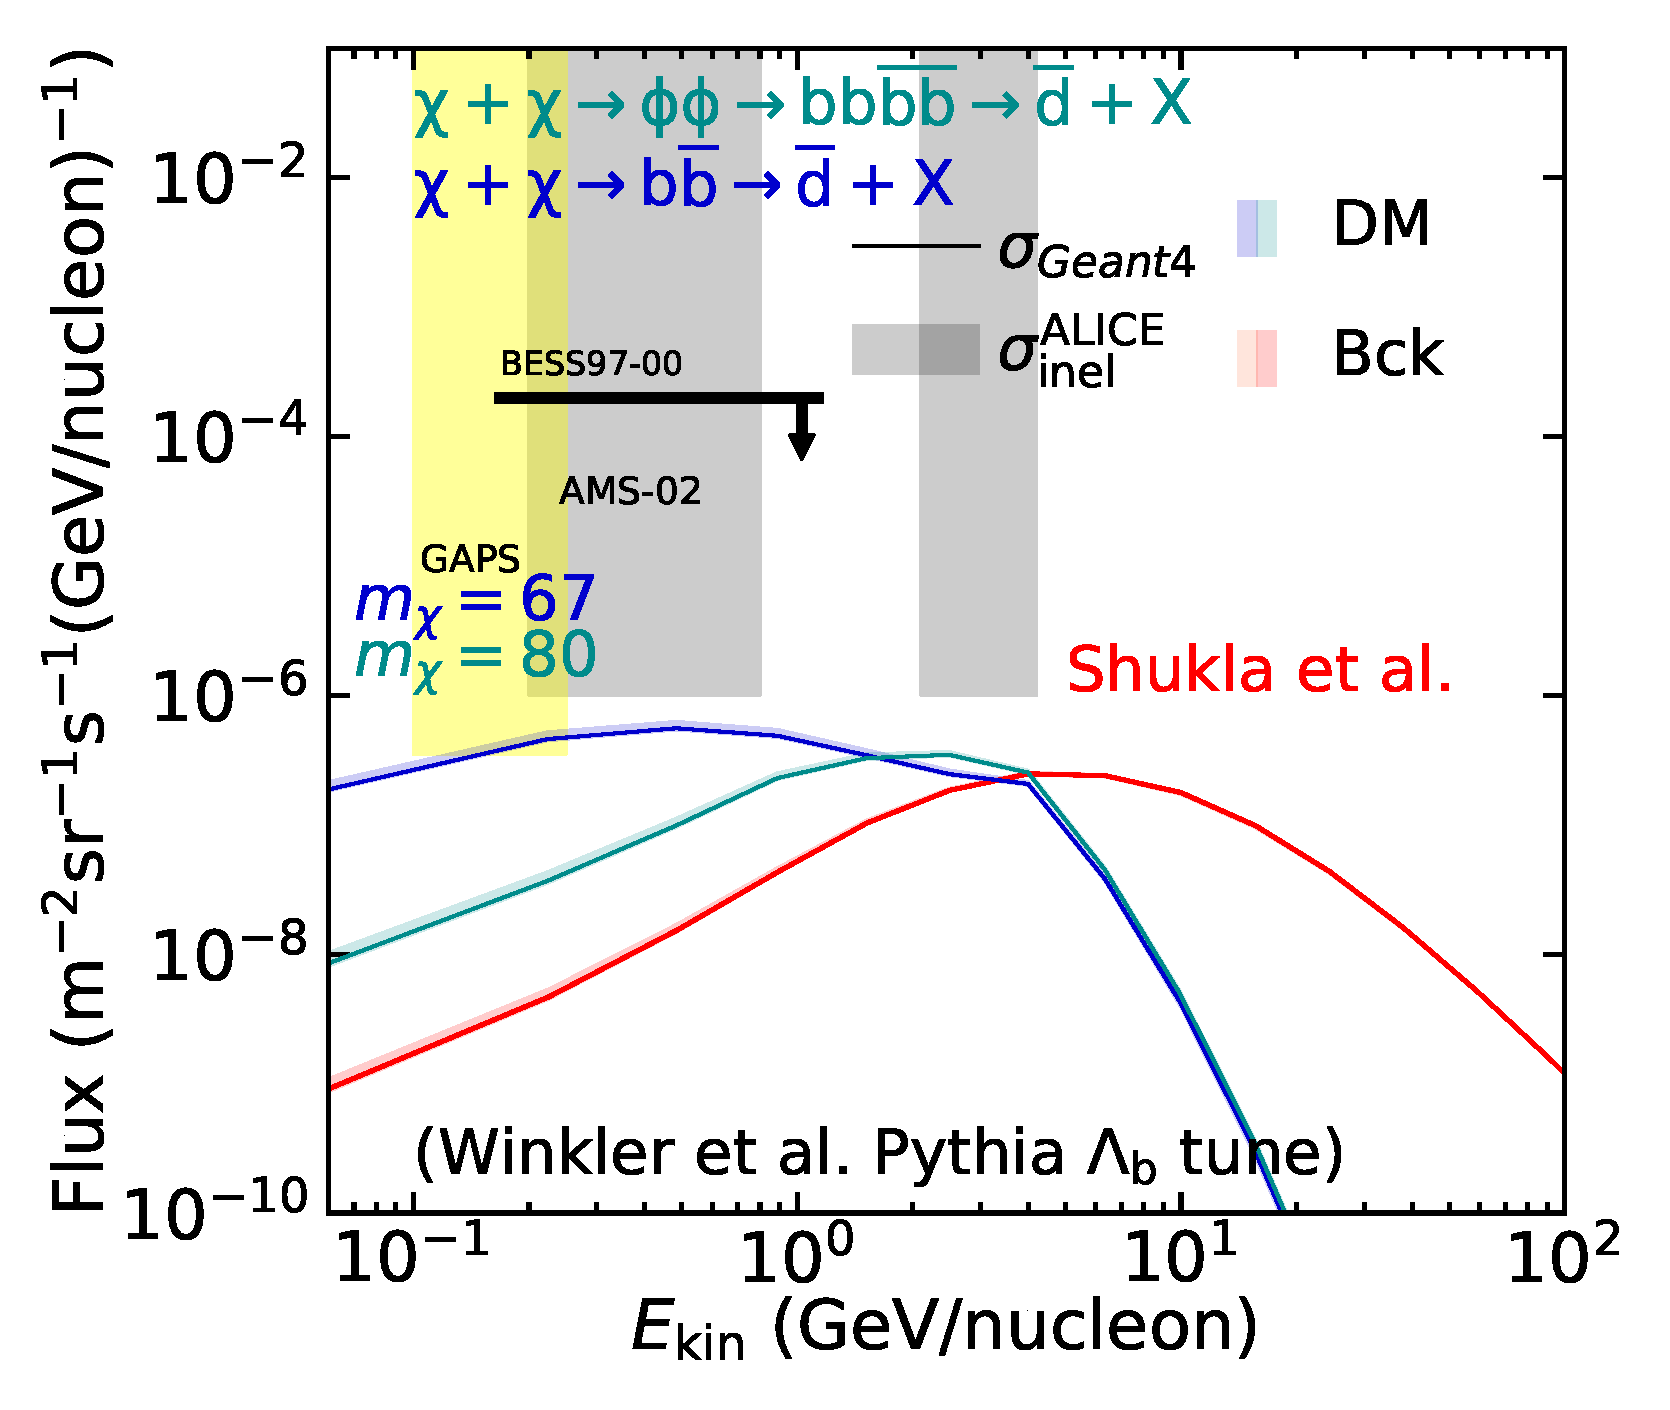
\includegraphics[width=0.49\textwidth]{figures/antideuteron_lambdaB_TOA.pdf}
    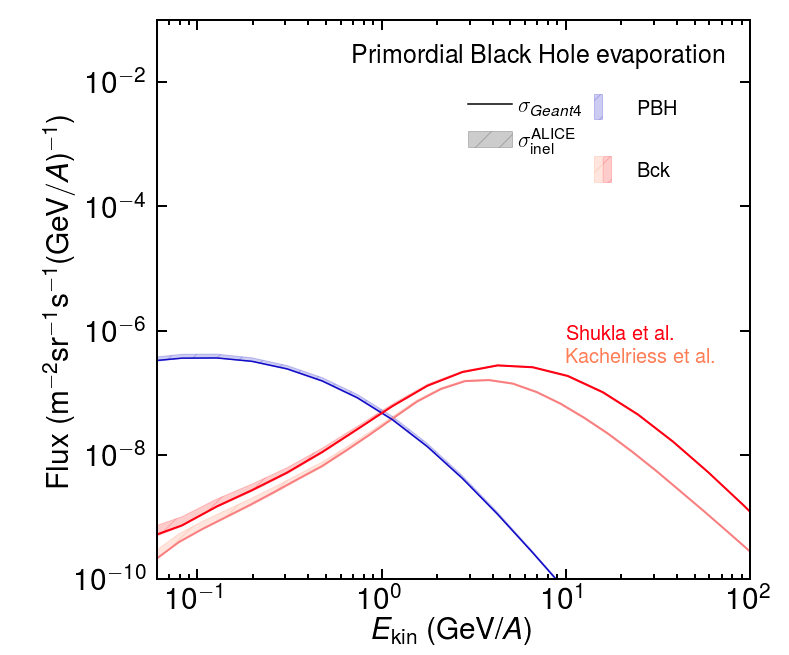
\includegraphics[width=.49\textwidth]{figures/antideuteron_fluxes_PBH_LIS.png}
    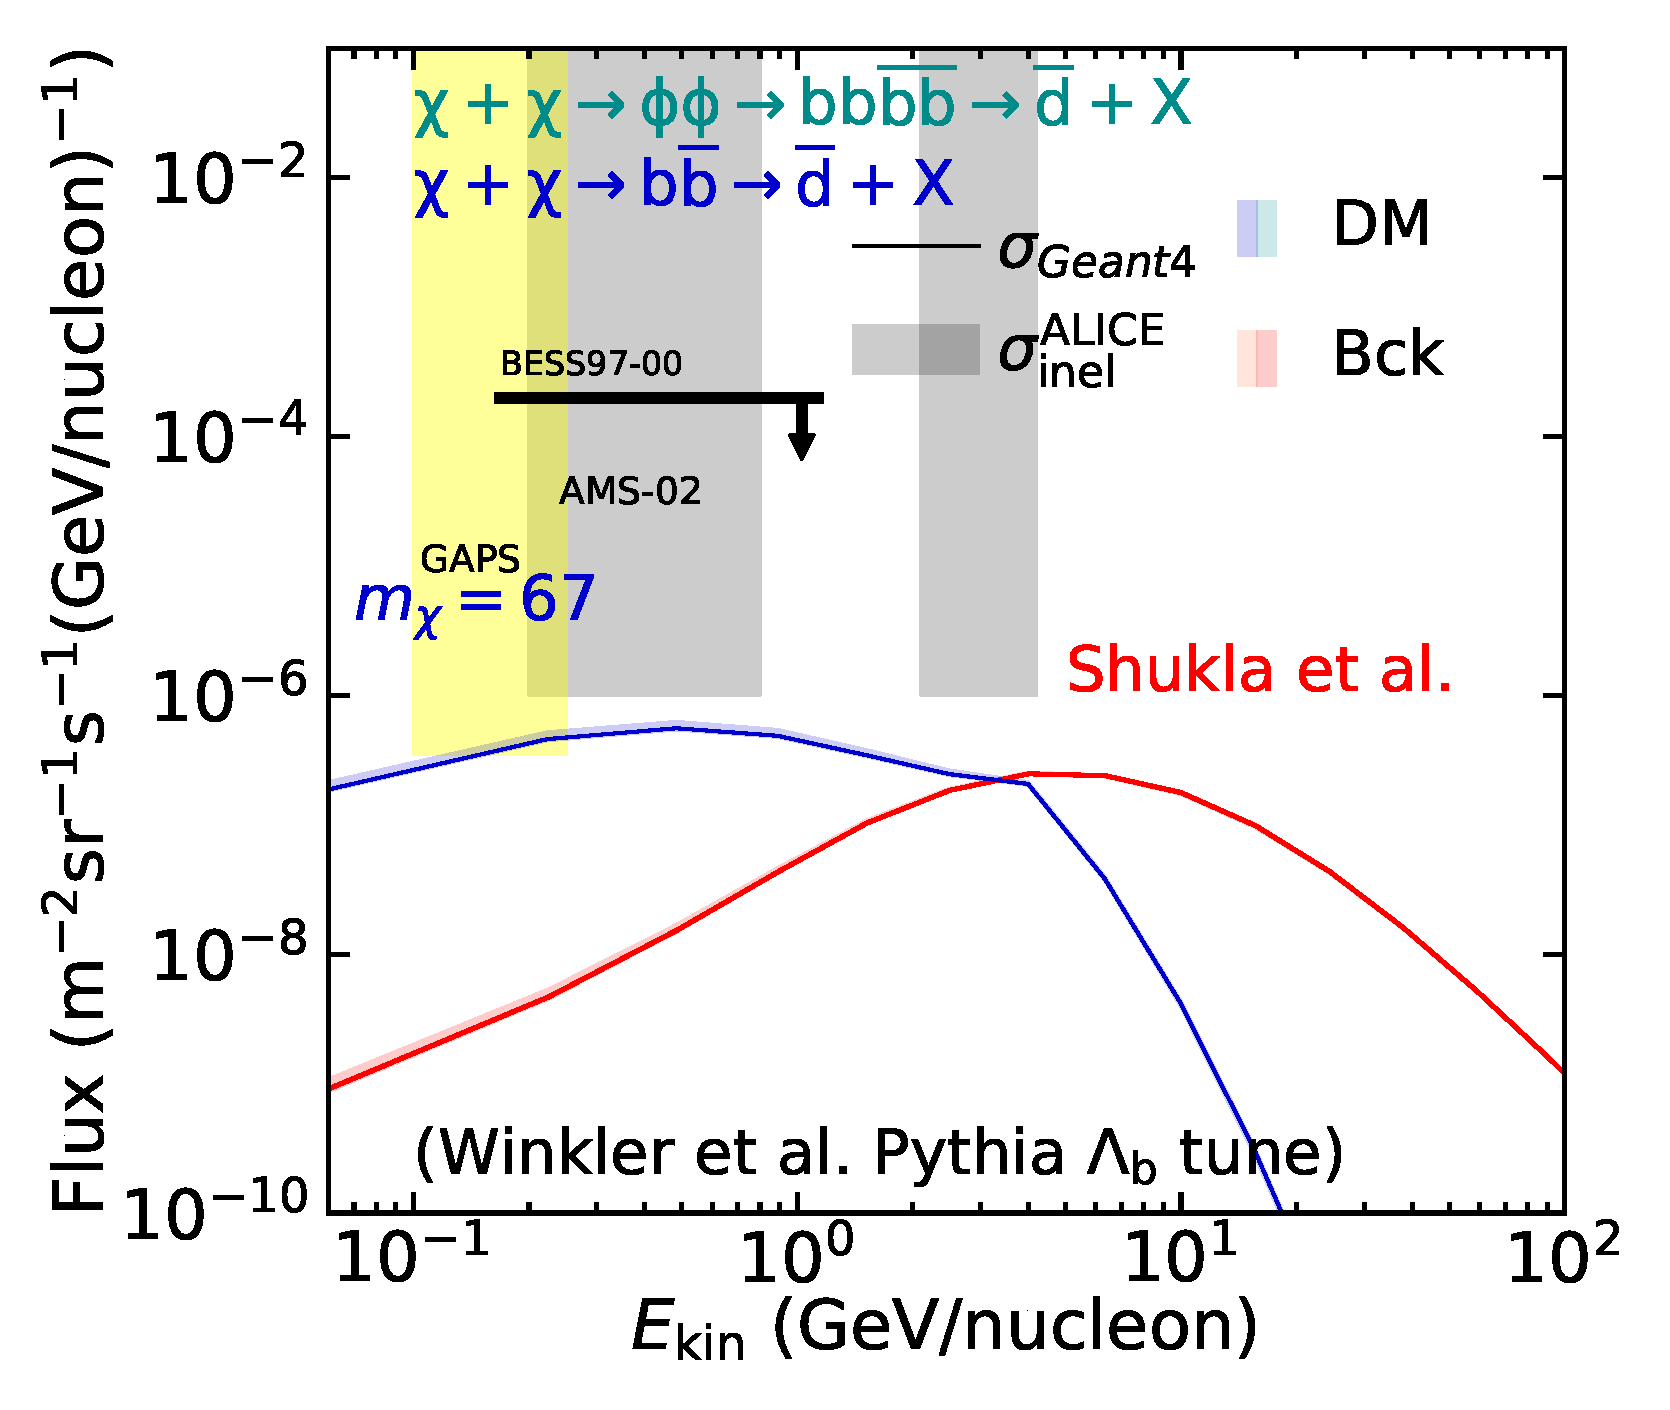
\includegraphics[width=.49\textwidth]{figures/antideuteron_TOA_LambdaB.pdf}
    \caption{Expected antideuteron fluxes for different \dmm\ ranging from 10 GeV to 1 TeV, and from primordial black holes (PBHs). They are compared to an expected spectrum of secondary antideuterons from high-energy cosmic-ray collisions. The results are shown for the position of the solar system. The figures on the left show the results without solar modulation, and on the right with solar modulation included by means of a force field model, as is discussed in section \ref{sec:Propagation}. The results are also shown for different possible annihilation channels of dark matter, either through \WW\ (top), through \bb\ (second from top), through $\Lambda_b \rightarrow $\bb\ and light mediators (third from top) and from PBHs (bottom).}
    \label{fig:Results_dbar_fluxes_diff_DM_masses}
\end{figure}

\subsubsection{Results for \ahe\ }
In this section the results for antihelium-3 fluxes using different dark matter masses \dmm\ are shown and discussed. These masses range over 2 orders of magnitude from 10 GeV all the way to 2 TeV, all of which are valid hypotheses for WIMP masses. As can be seen in figure \ref{fig:Results_He3_fluxes_diff_DM_masses}, the result is not just a difference in the overall normalization, but also in the shape of the produced spectrum. This is because the larger energy available with the higher mass translates into more kinetic energy in the final state particles, i.e. the produced antinuclei. It can also be seen that the increased production with increased mass does not compensate for the reduction in annihilation rate due to the lower number density\footnote{This is the 1/$m_\chi^2$ scaling seen in equation \ref{eq:DM_source_term}.}, thus the magnitude of the flux decreases with increasing dark matter mass. Also shown in the bottom panel for each figure, is the transparency of the galaxy to \ahe\, defined in equation \ref{eq:TransparencyDefinition}. It is promising that the predicted fluxes from $\overline{\Lambda}_b$ decays in figure \ref{fig:Results_He3_fluxes_diff_DM_masses} reach the AMS-02 sensitivities even without accounting for other uncertainties. For other channels, a boost of about 1-2 orders of magnitude is possible in the most optimistic scenario, as can be seen from table \ref{tab:uncertaintiesFluxes}, which could potentially allow a signal in both the \bb\ and \WW\ channels for masses of around \dmm\ = 100 GeV. And even a null observation would place more and more stringent limits on dark matter models, further tightening the available parameter space. 

\begin{figure}[hbtp]
    \centering
    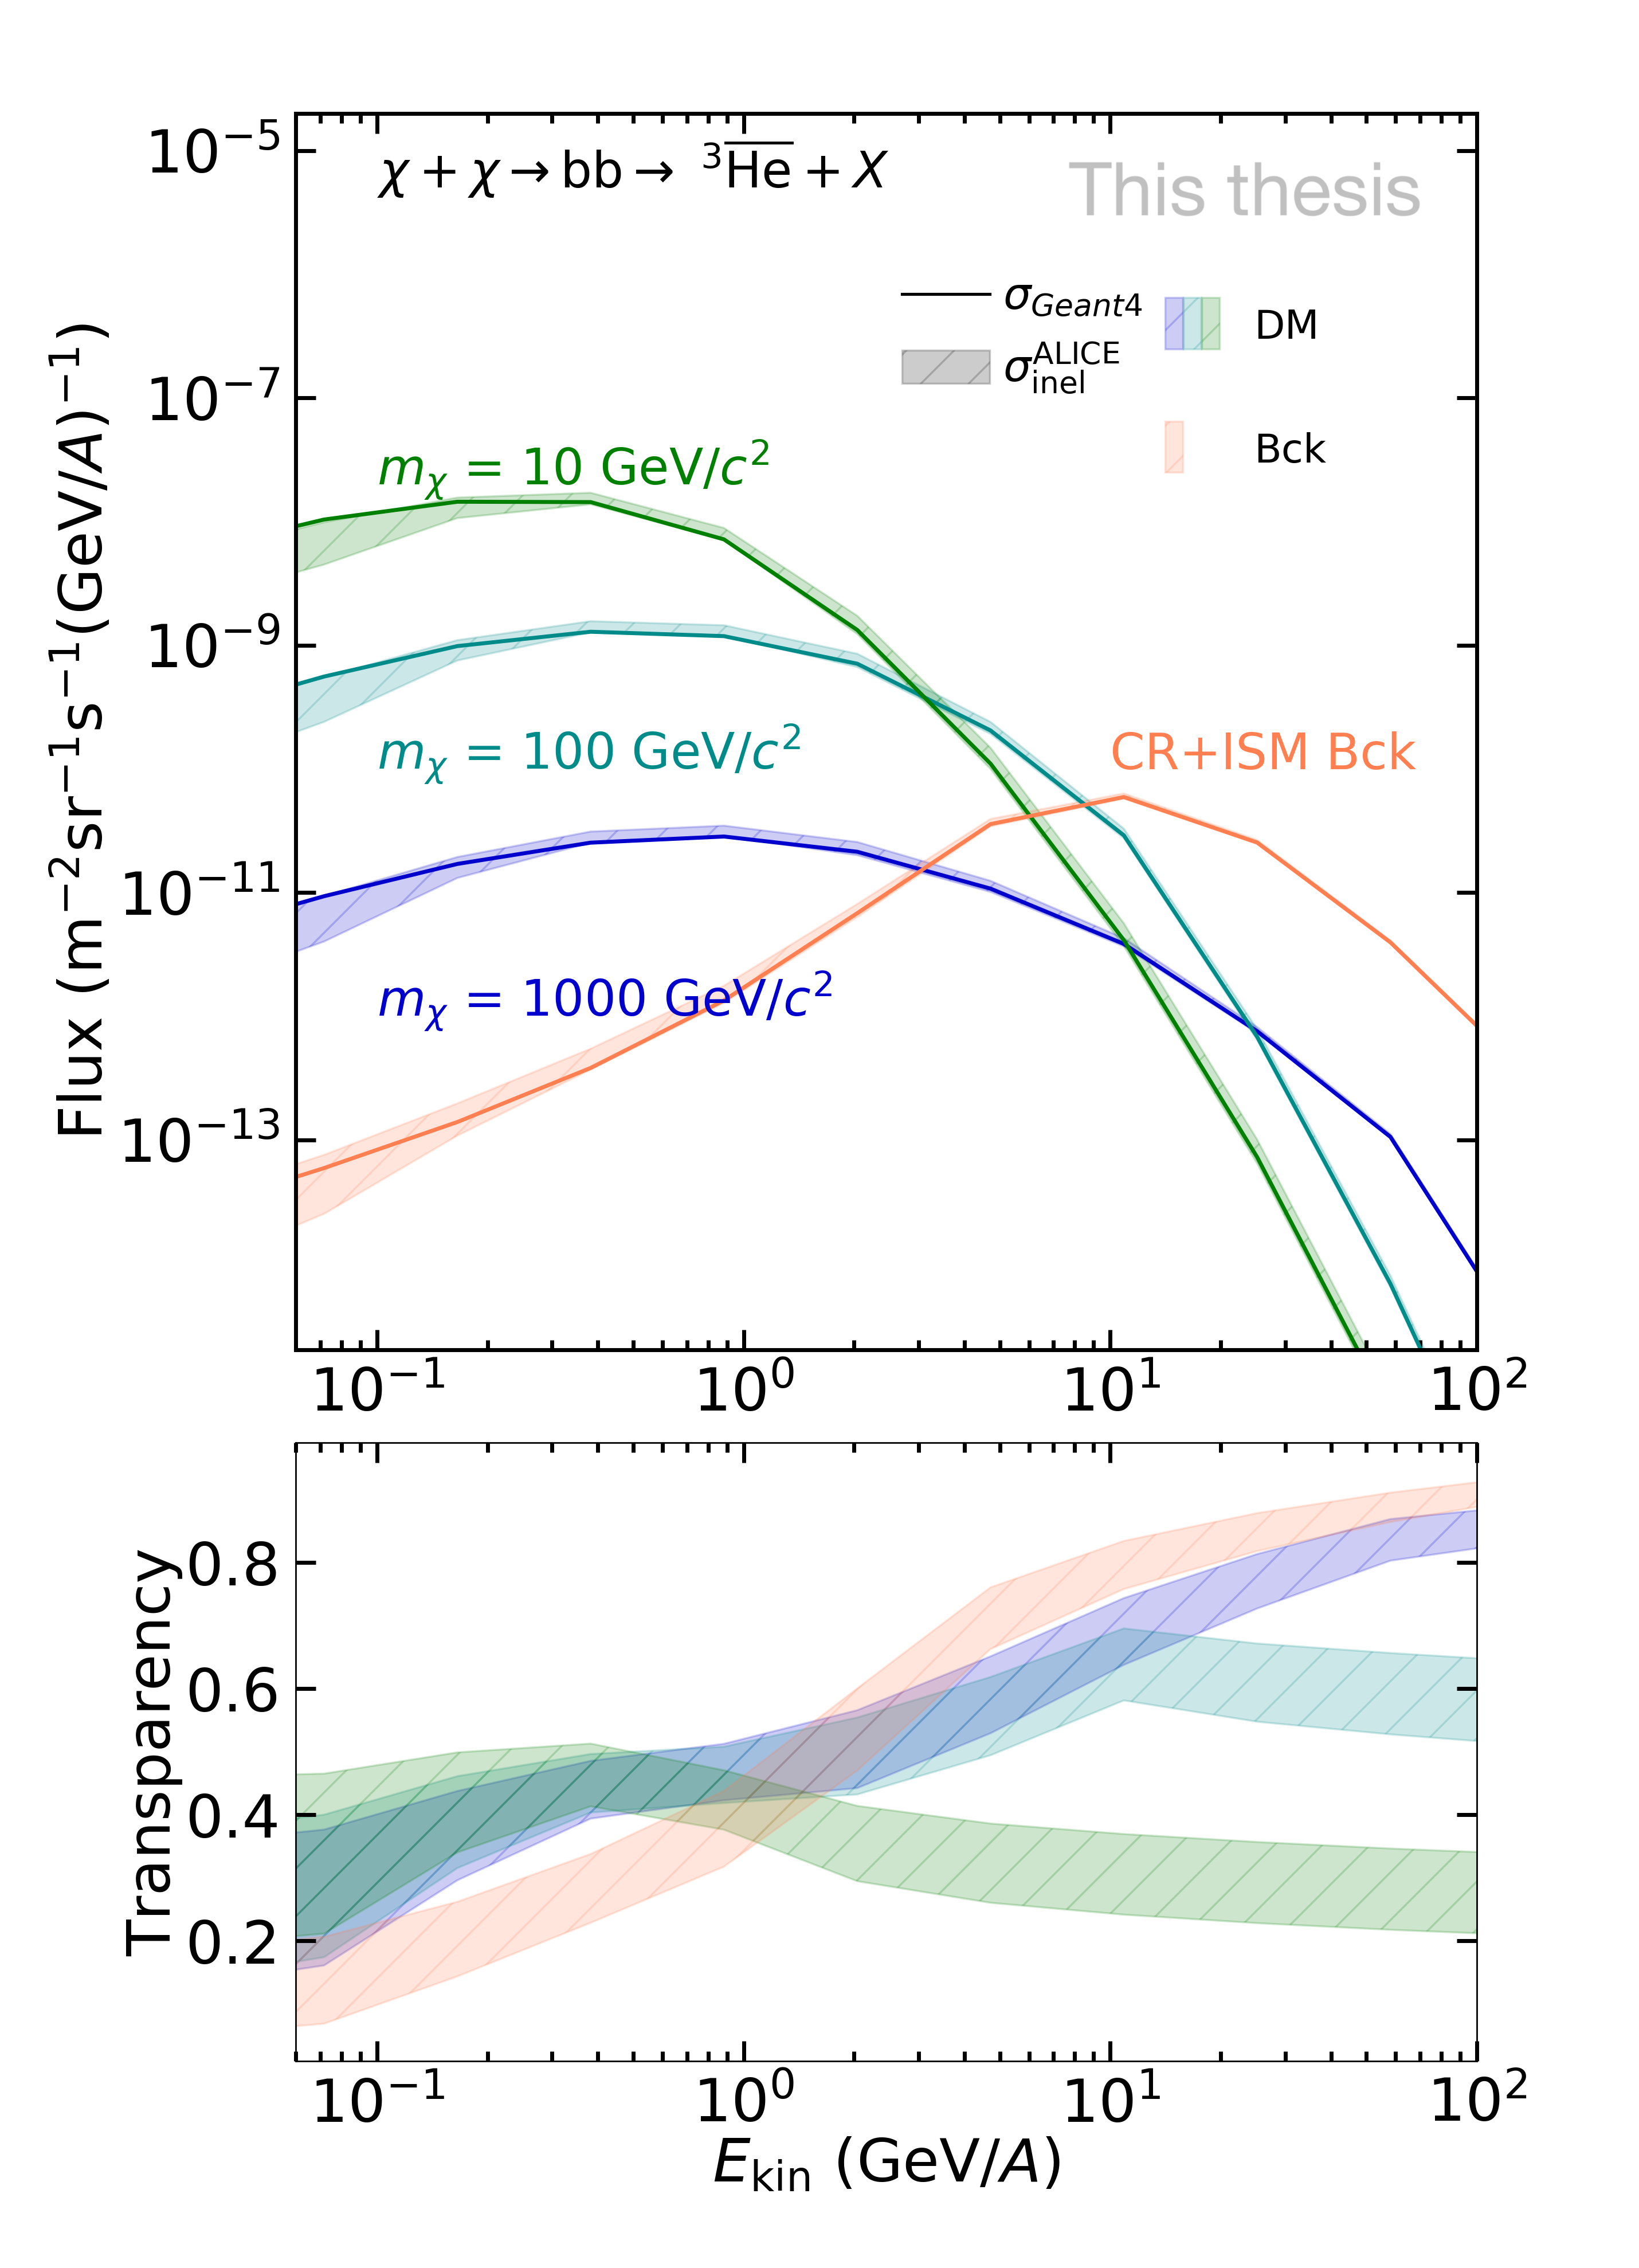
\includegraphics[width=0.49\textwidth]{figures/he3bar_bb_LIS.png}
    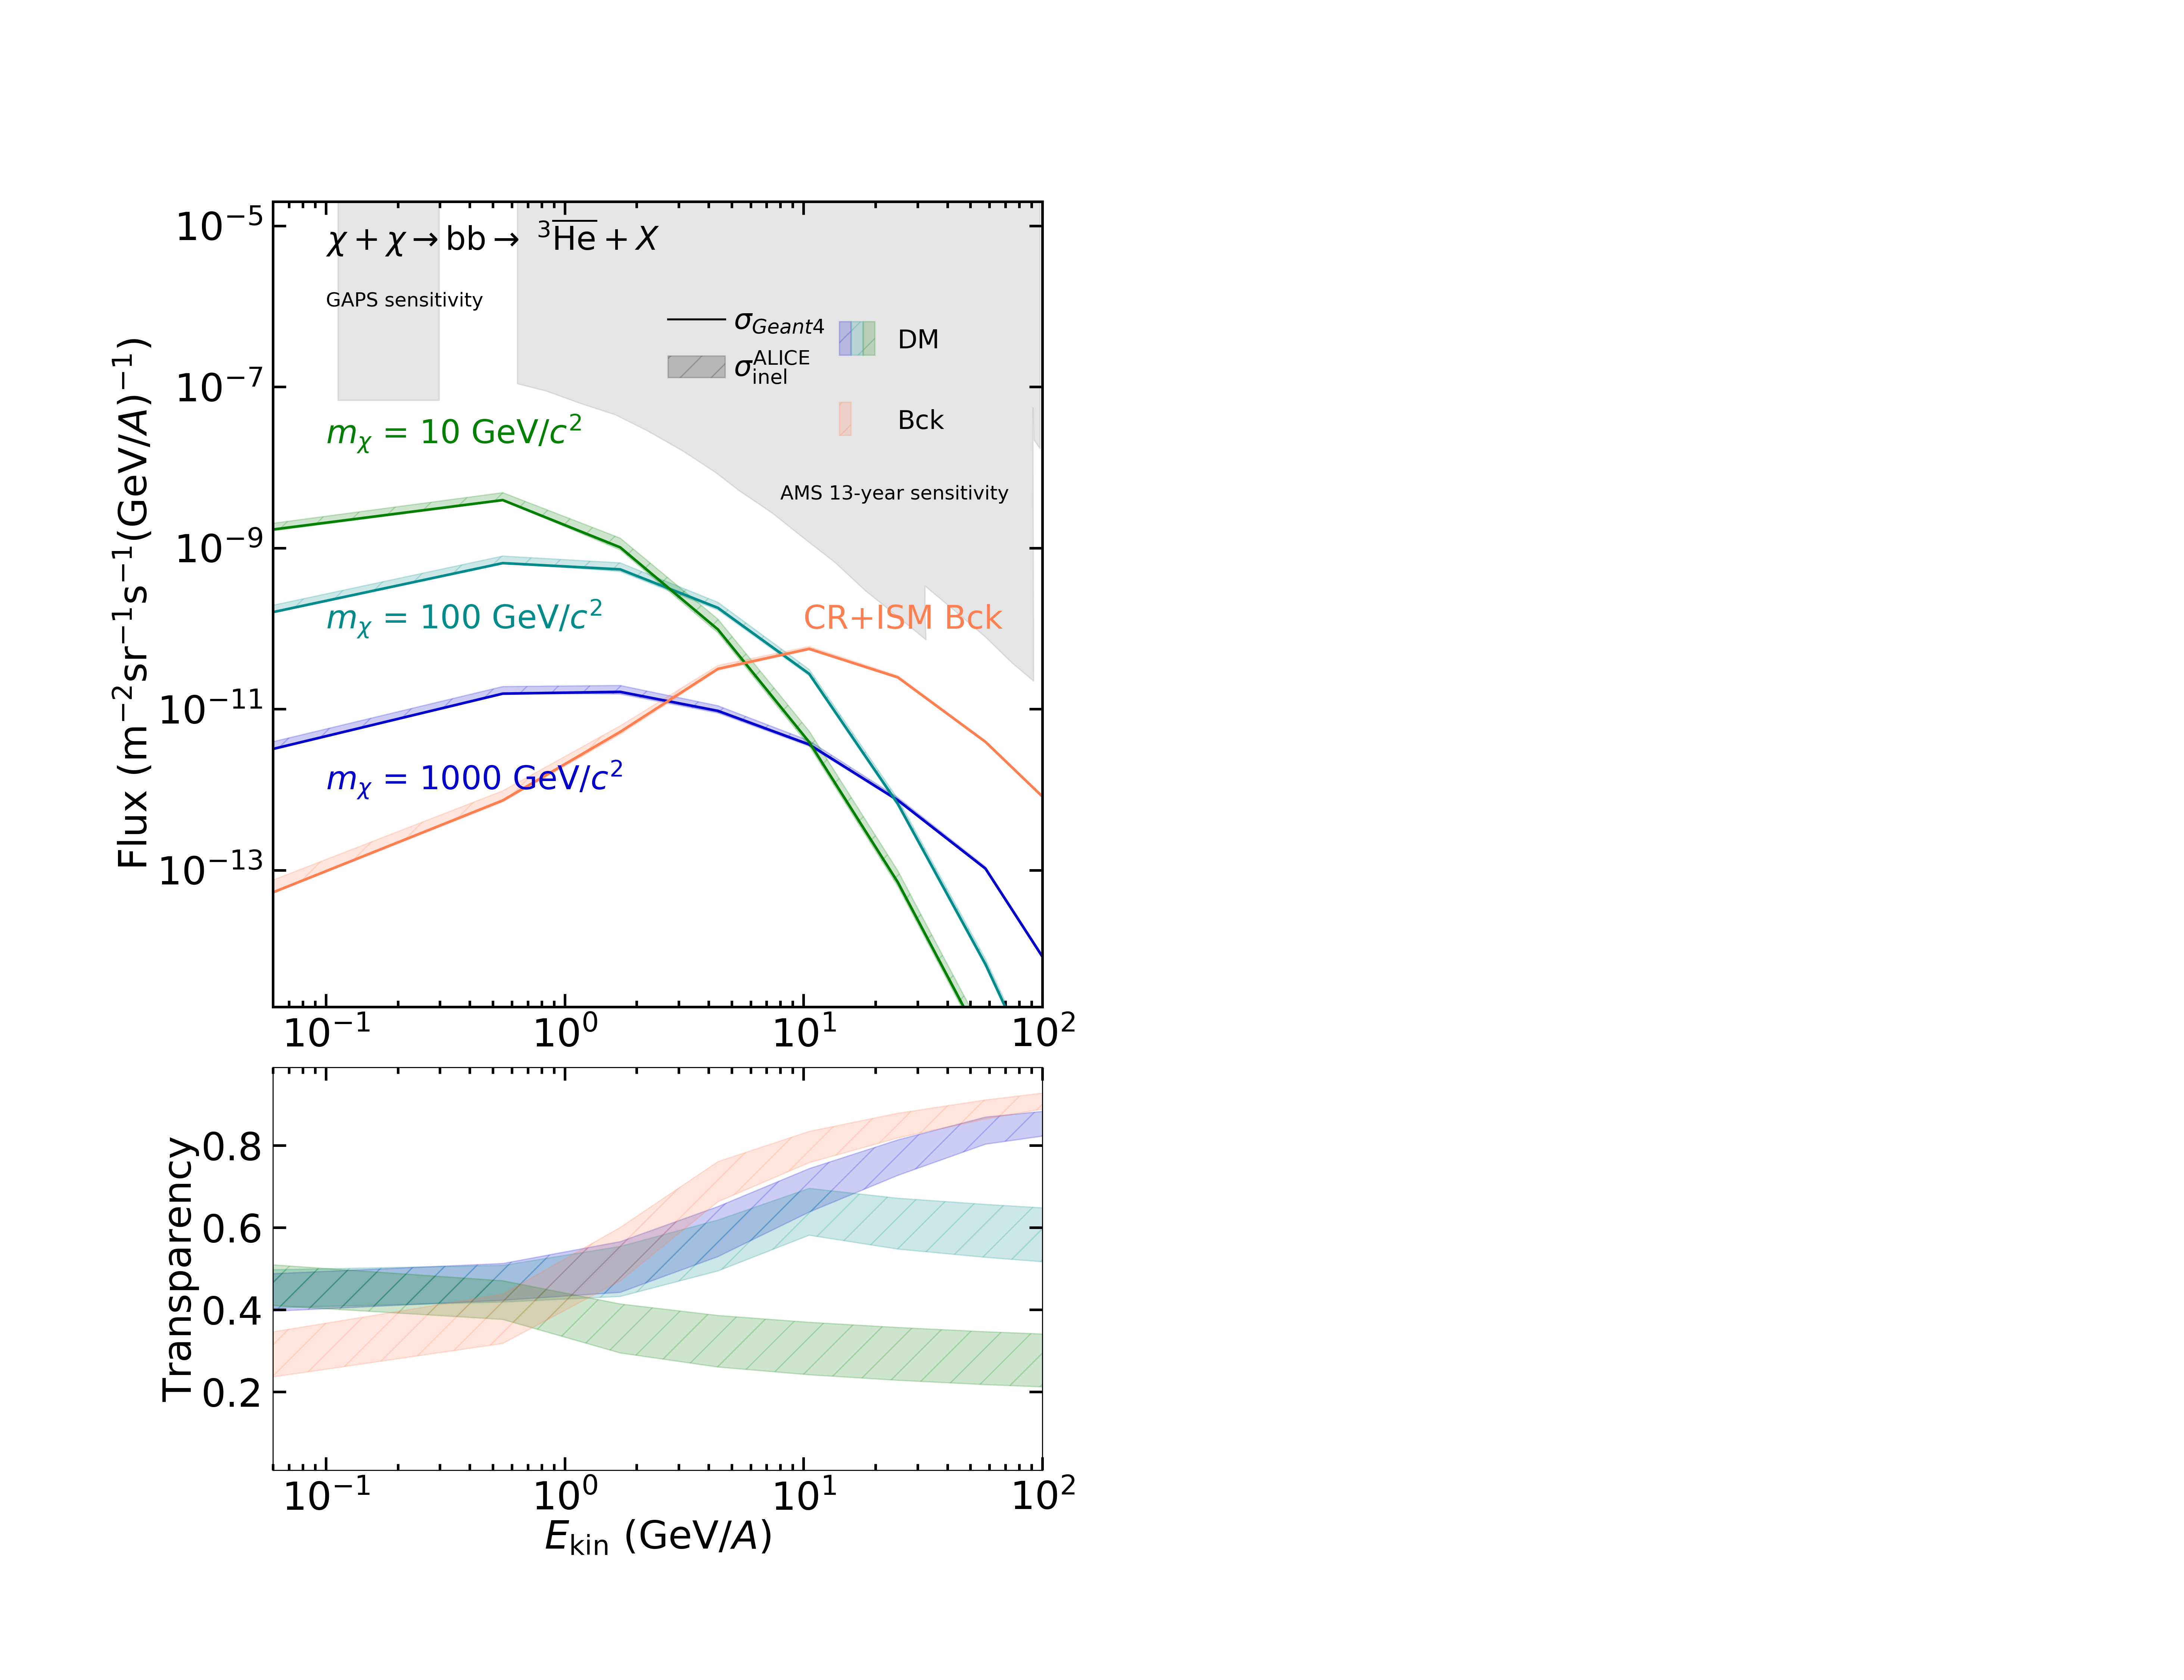
\includegraphics[width=0.49\textwidth]{figures/he3bar_bb_SM.png}
    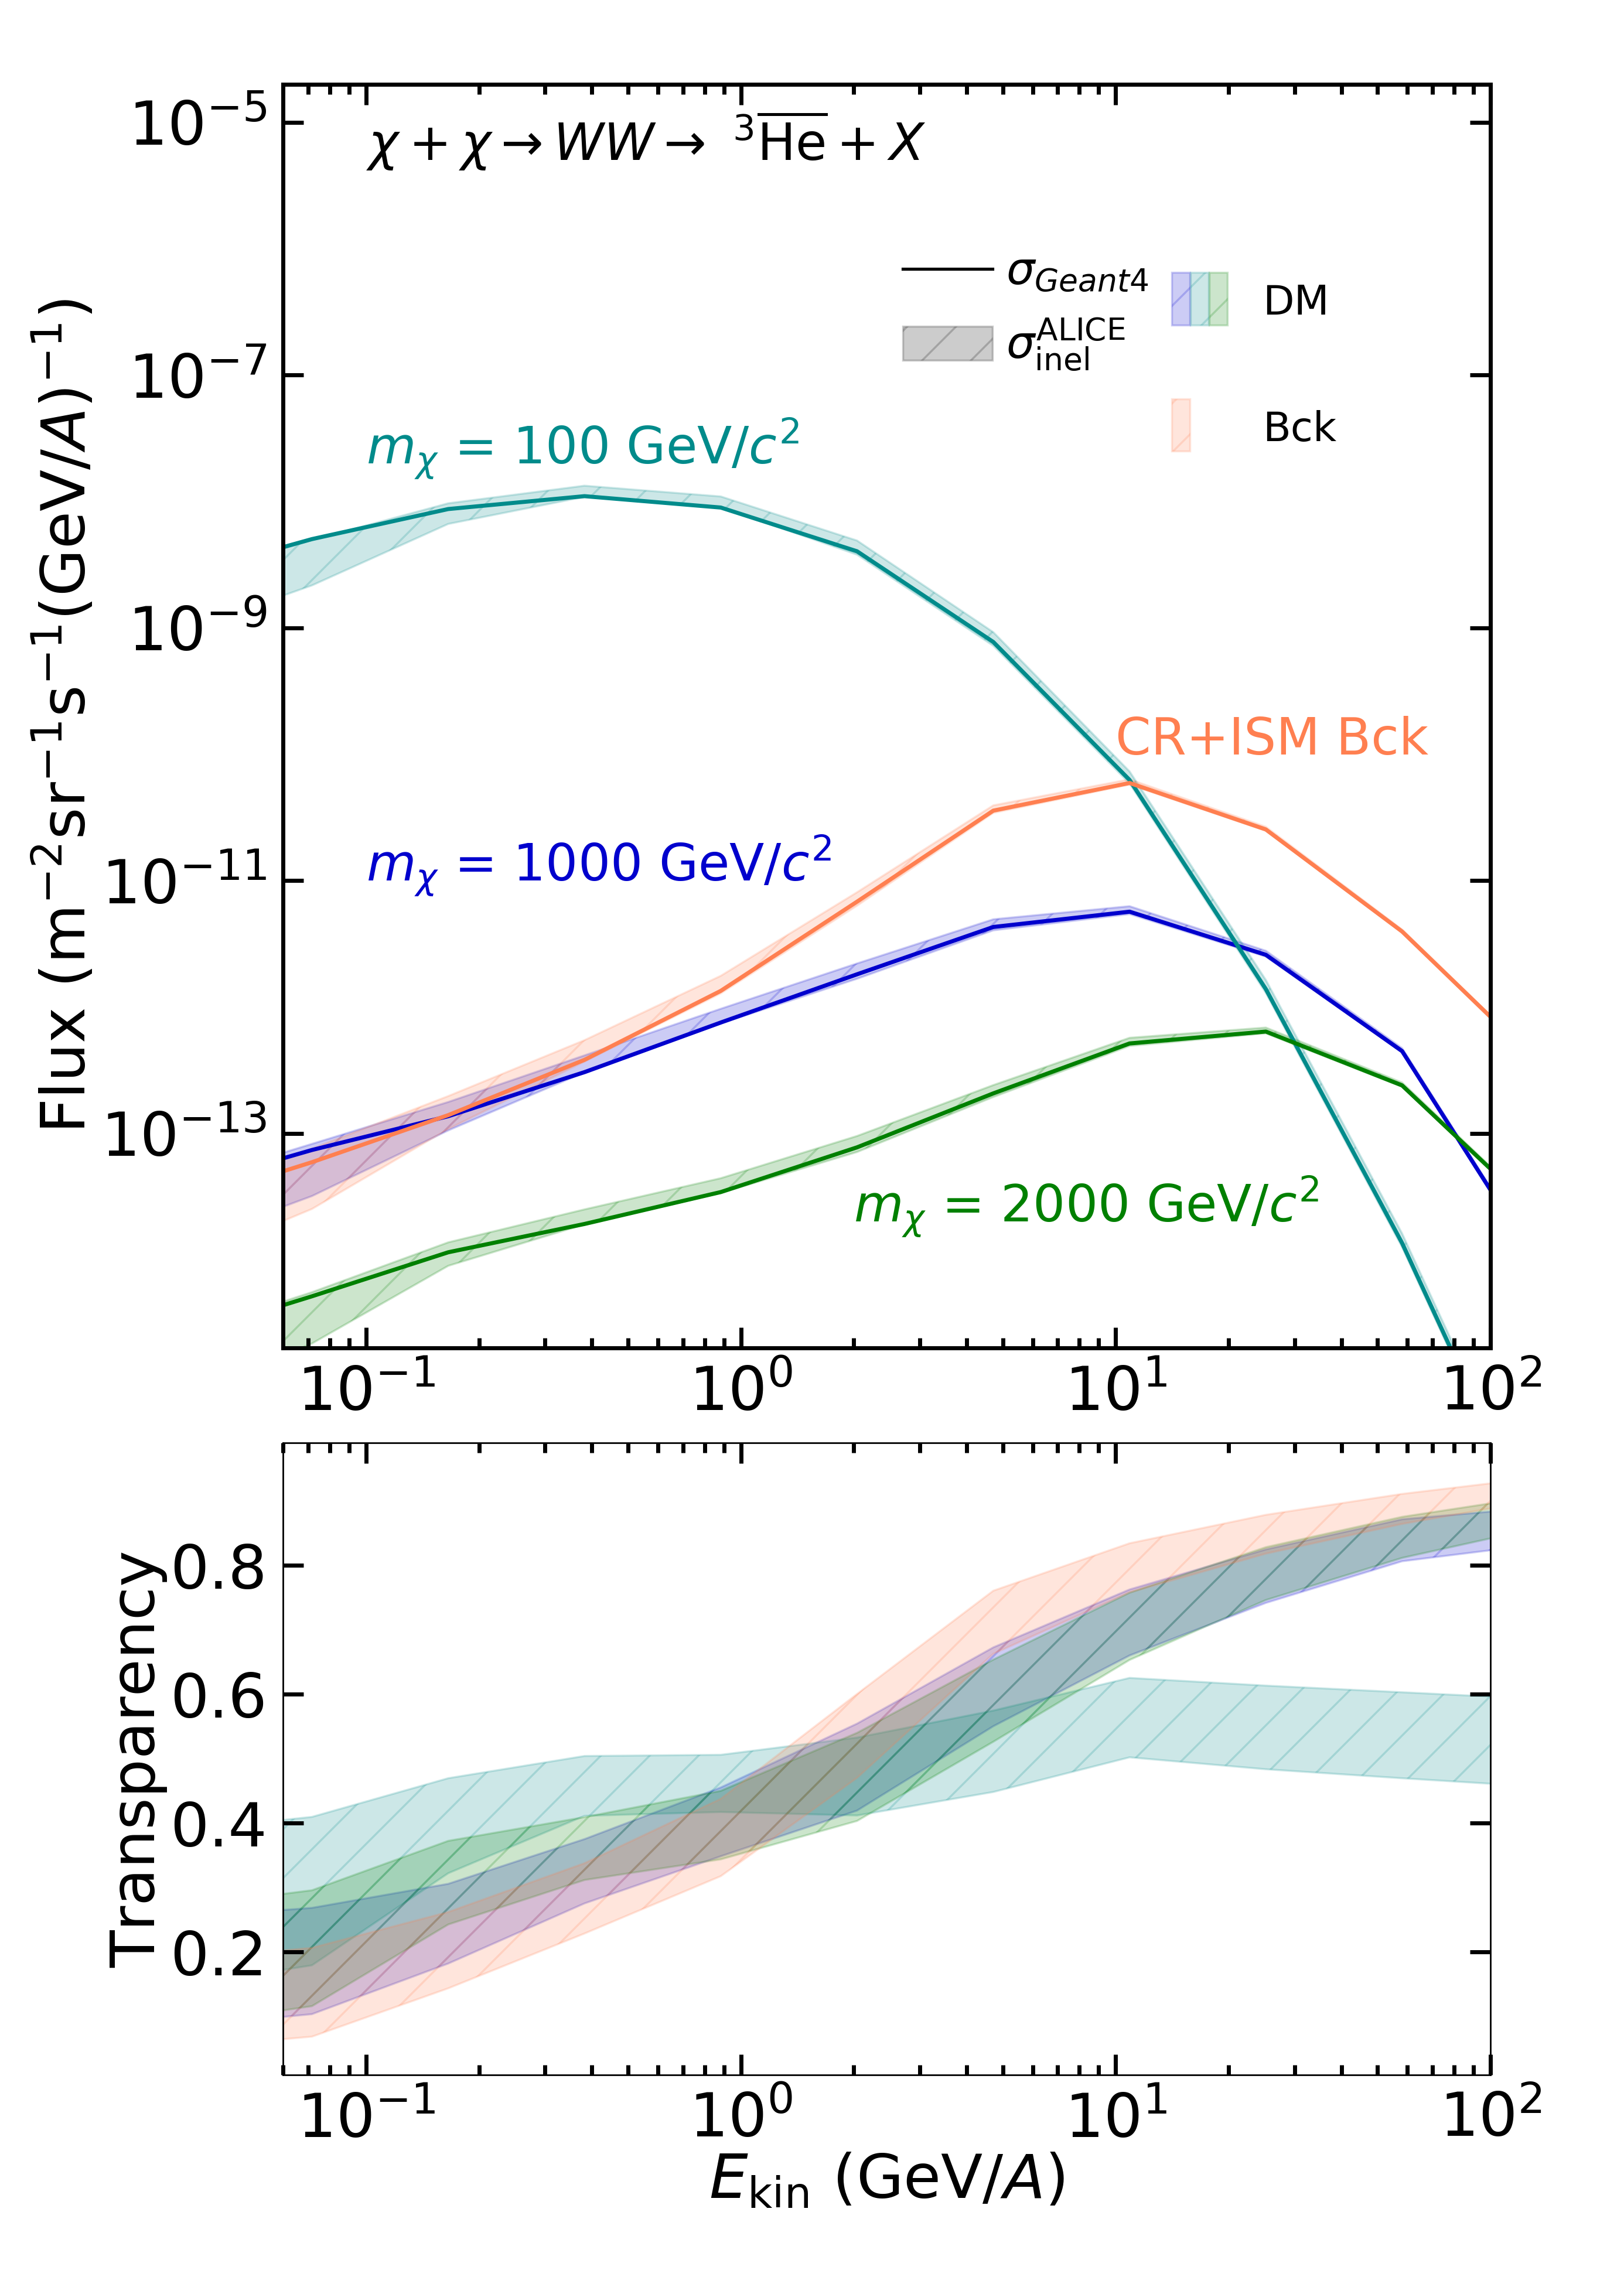
\includegraphics[width=0.49\textwidth]{figures/he3bar_WW_LIS.png}
    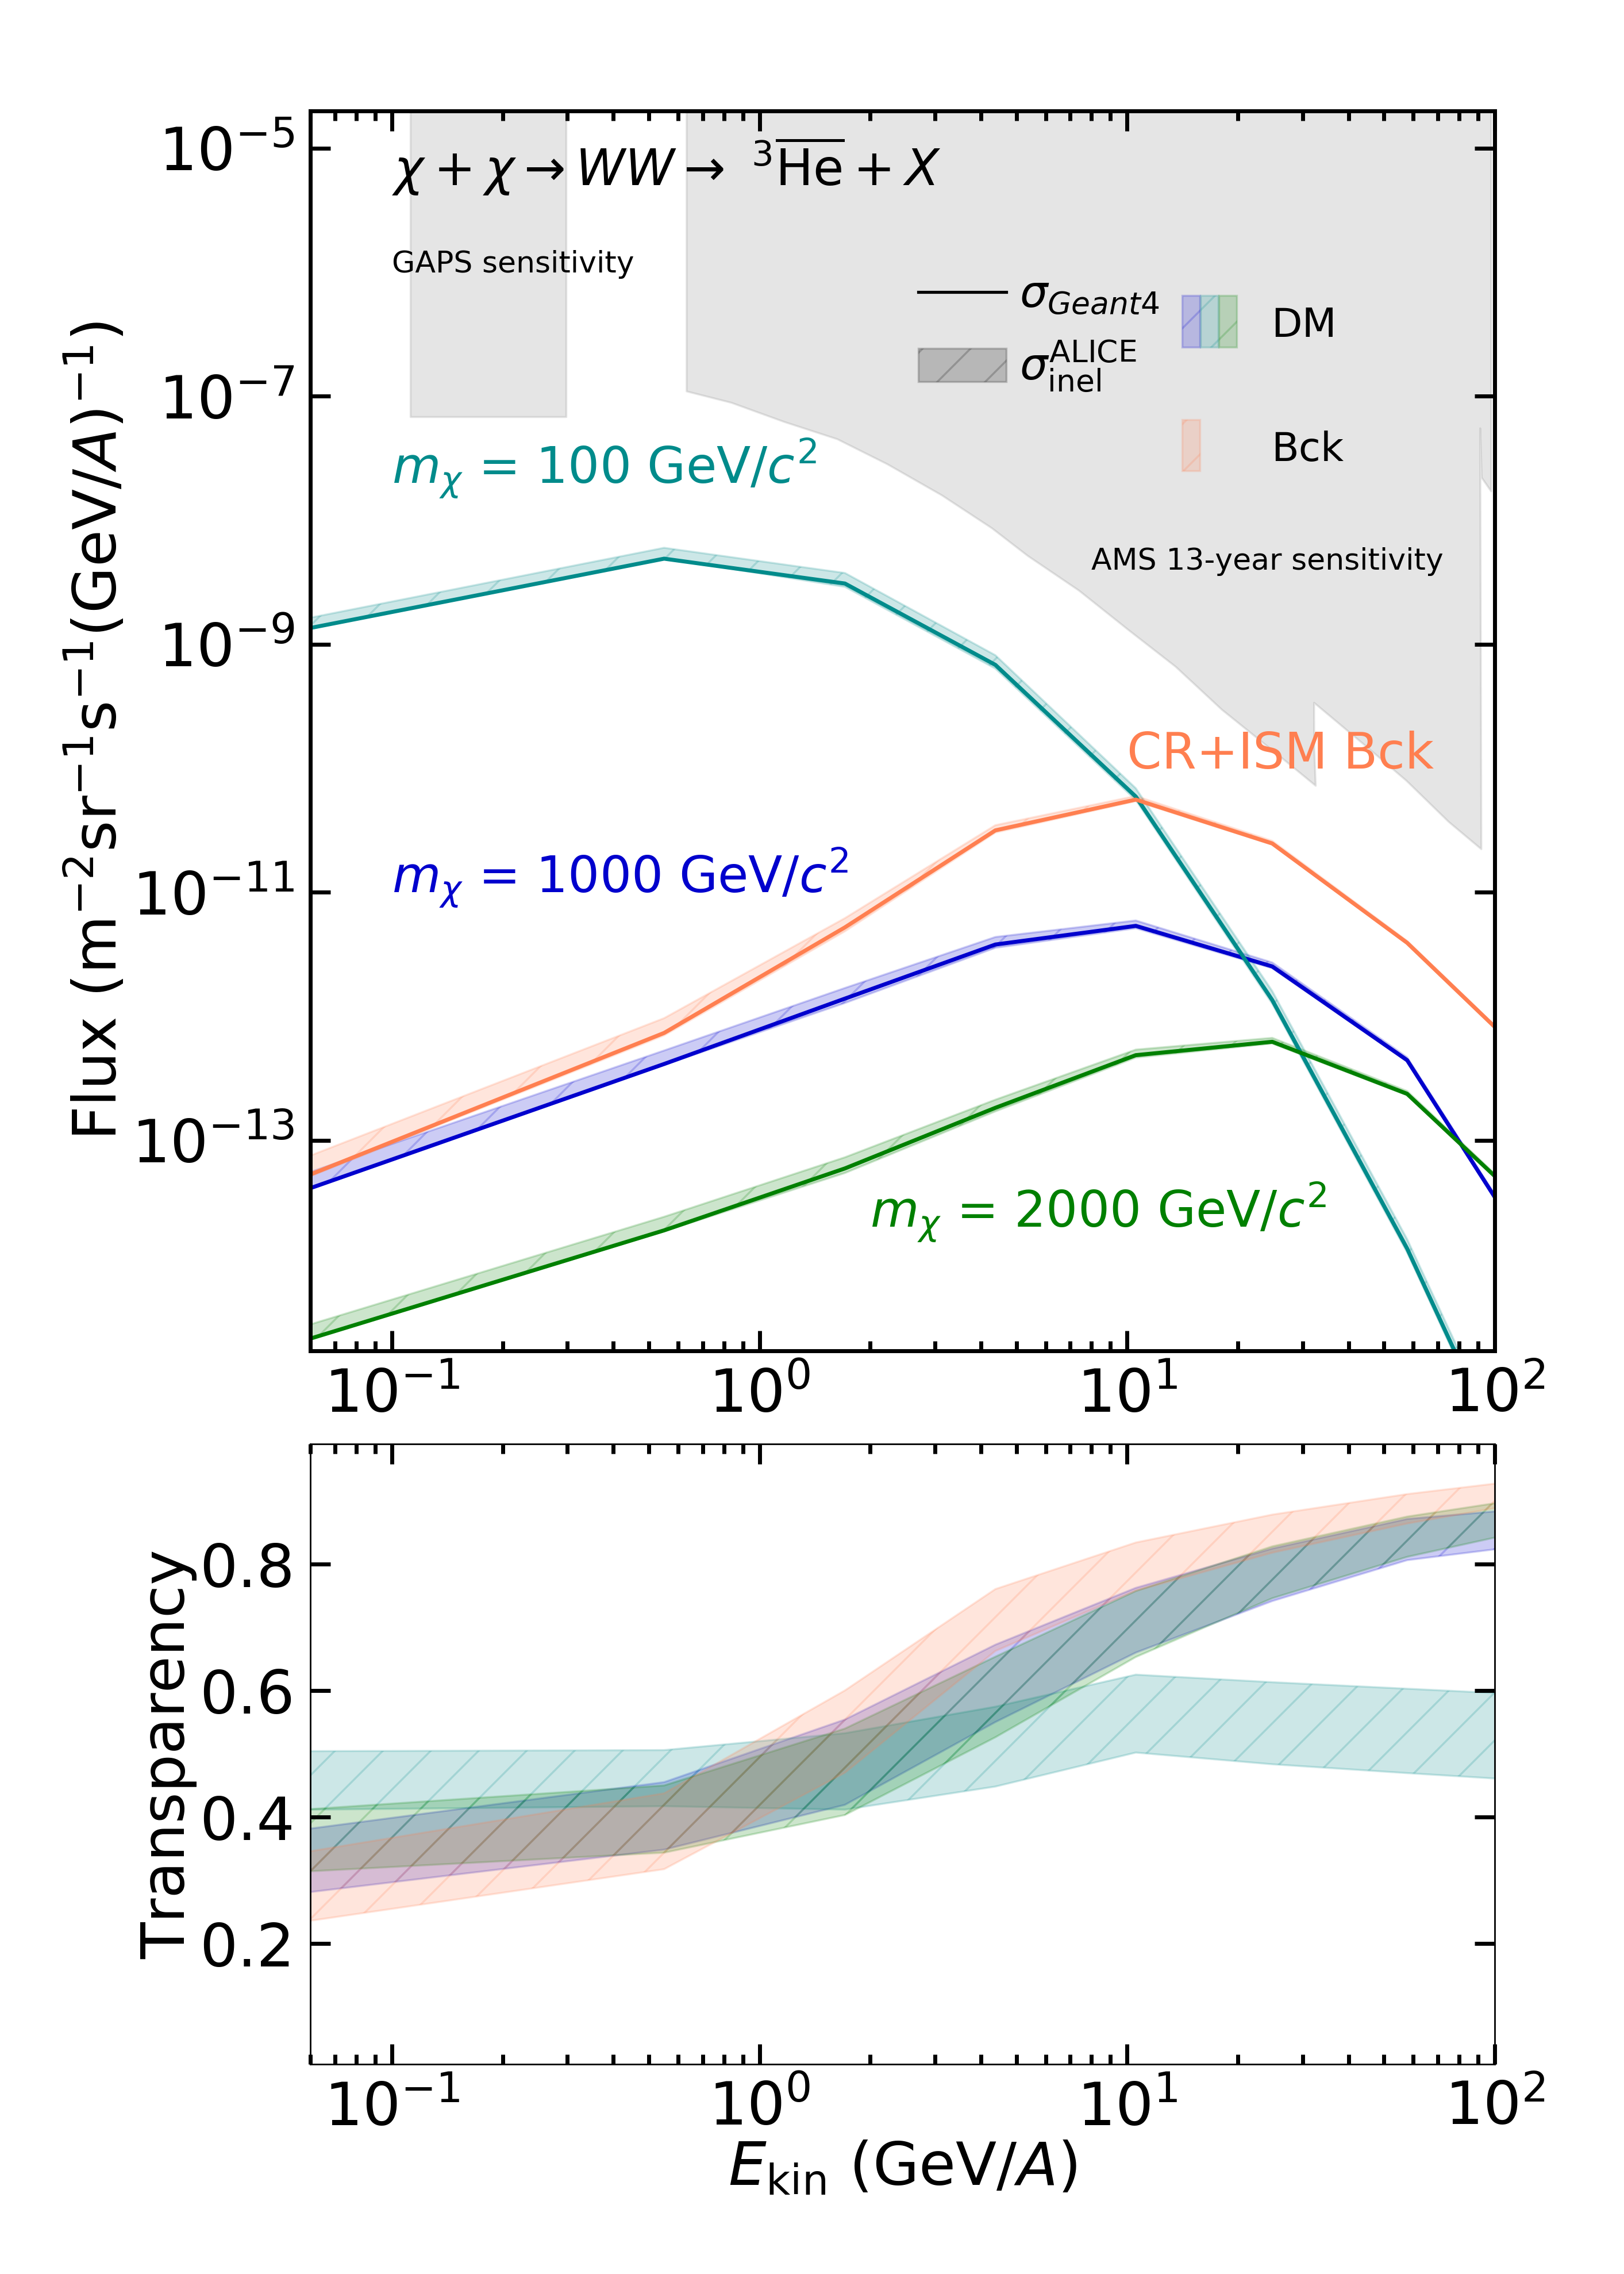
\includegraphics[width=0.49\textwidth]{figures/he3bar_WW_SM.png}
    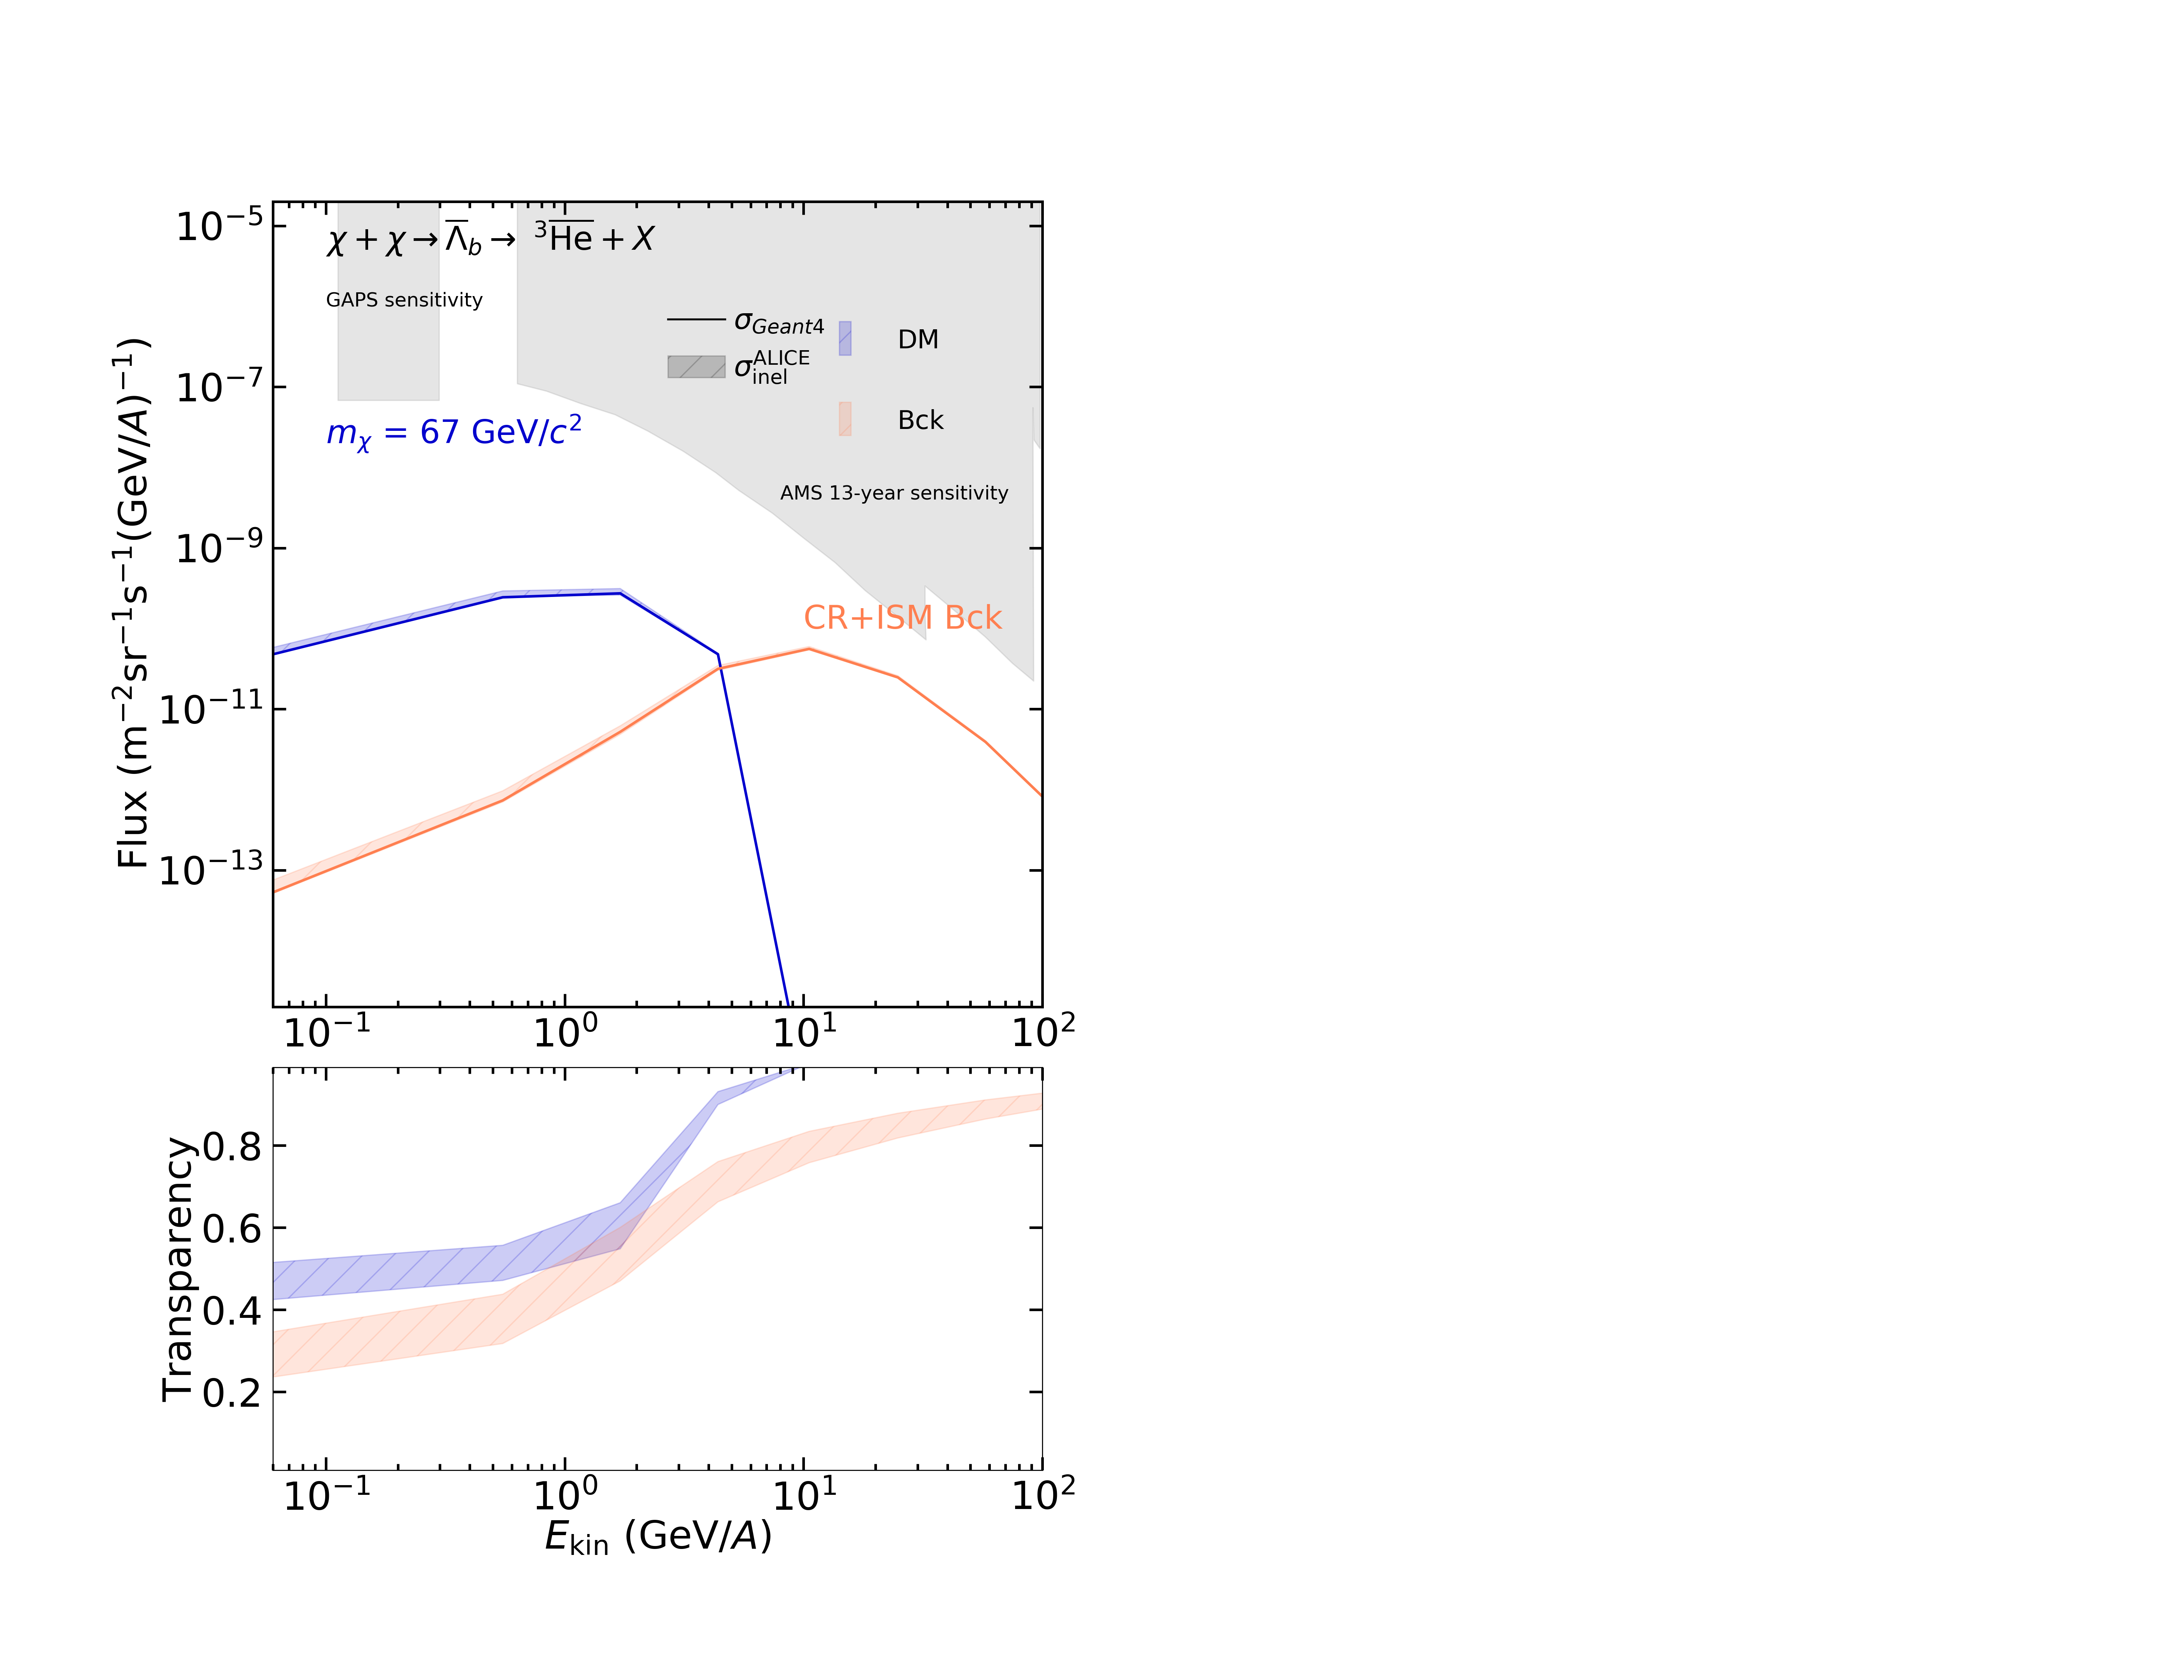
\includegraphics[width=0.49\textwidth]{figures/he3bar_LambdaB_LIS.png}
    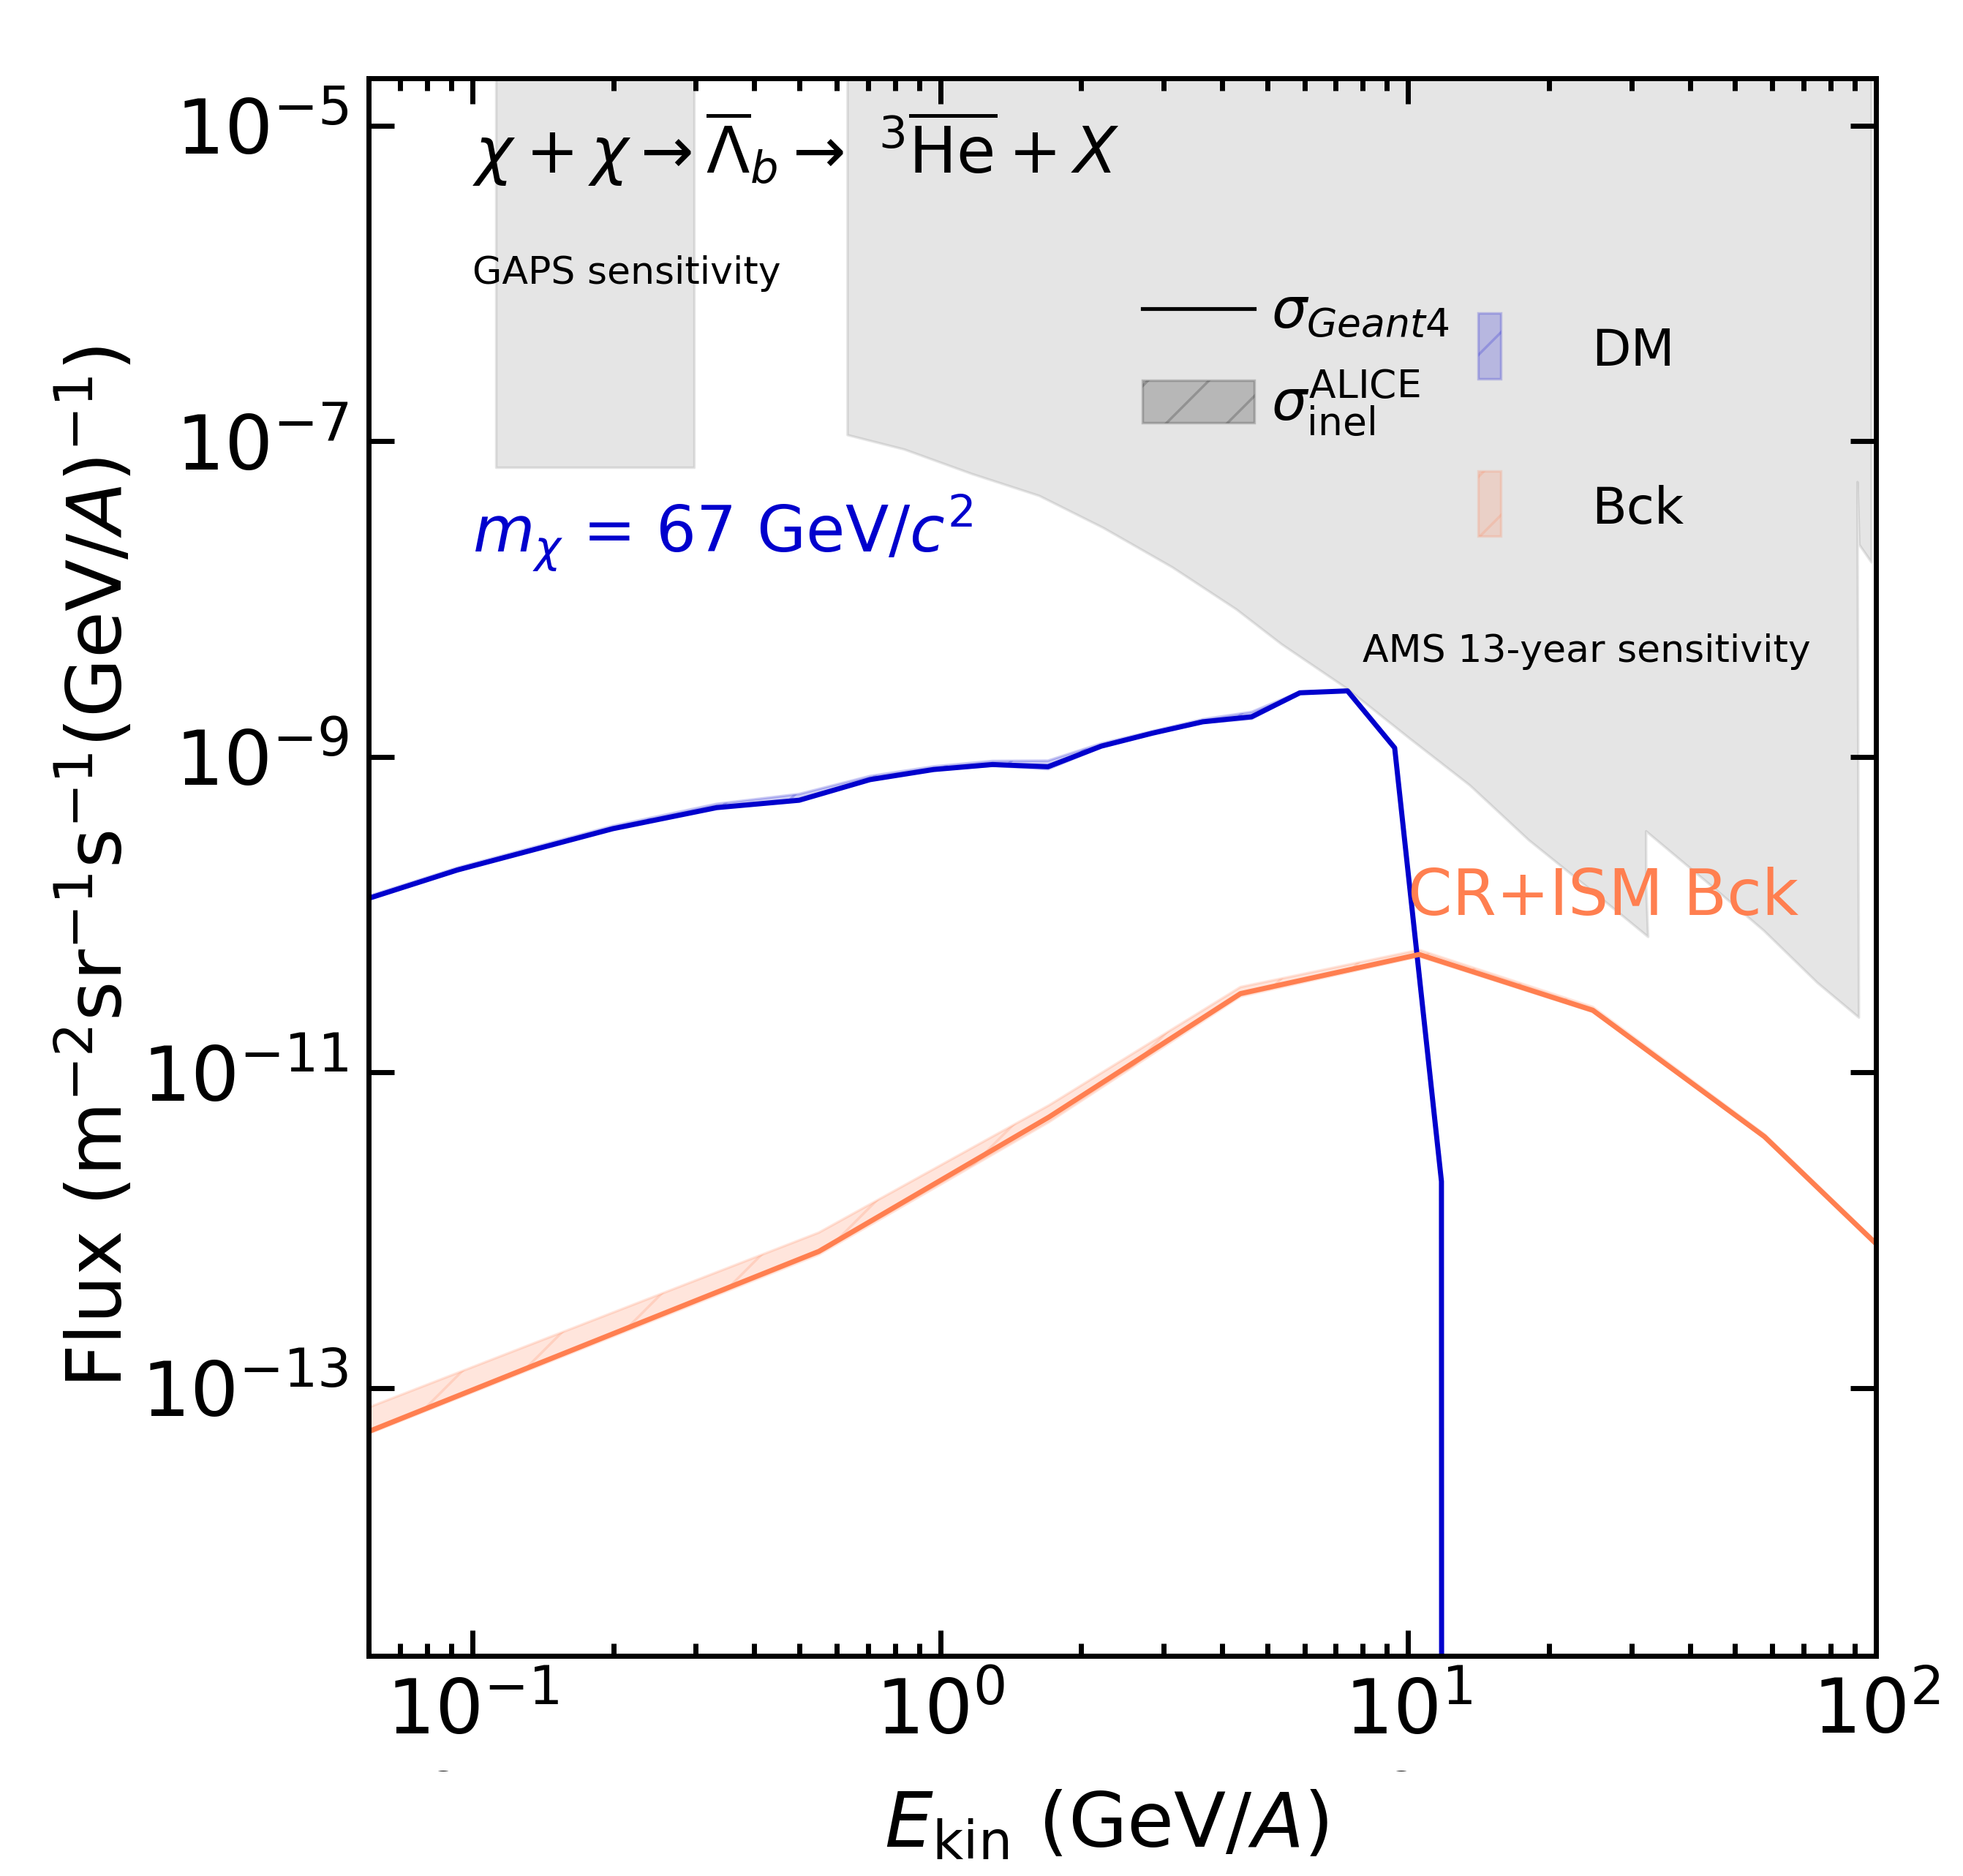
\includegraphics[width=0.49\textwidth]{figures/he3bar_LambdaB_TOA_fine.png}
    \caption{Expected \ahe\ fluxes for different \dmm\ ranging from 1GeV to 2TeV. They are compared to an expected spectrum of secondary \ahe\ from high energy cosmic ray collisions. The results are shown for the position of the solar system. The figures on the left show the results without solar modulation, and on the right with solar modulation included by means of a force field model, as is discussed in section \ref{sec:Propagation}. The results are also shown for different possible annihilation channels of dark matter, either through \WW\ (top), through \bb\ (middle) or through $\overline{\Lambda}_b$ decays (bottom).}
    \label{fig:Results_He3_fluxes_diff_DM_masses}
\end{figure}

\subsection{Results for different dark matter profiles}\label{sec:ResDMProfiles}
The effect of the different dark matter profiles is shown only on one channel and one dark matter mass, since it has similar effects on all channels/masses. The absolute normalization is degenerate with bounds from antiproton measurements, as was discussed in section \ref{sec:WIMPS}. However, more insight can be gained from the bottom panels of figure \ref{fig:different_DM_profiles_and_transparencies}, where the transparency is shown. The transparency of the Milky Way shows a significant shift between the three different profiles. This can be understood as the mean distance that antinuclei from dark matter have to traverse in order to get to earth. The more peaked the profile is towards the center, the longer the mean path. This in turn reduces the transparency. Thus, the transparency of the galaxy to antinuclei is lowest for the Einasto profile, which is the most peaked, as can be seen in figure \ref{fig:DM_profiles}. It is highest for the isothermal profile, which is relatively flat towards the centre of the Milky Way. 

\begin{figure}[hbtp]
    \centering
    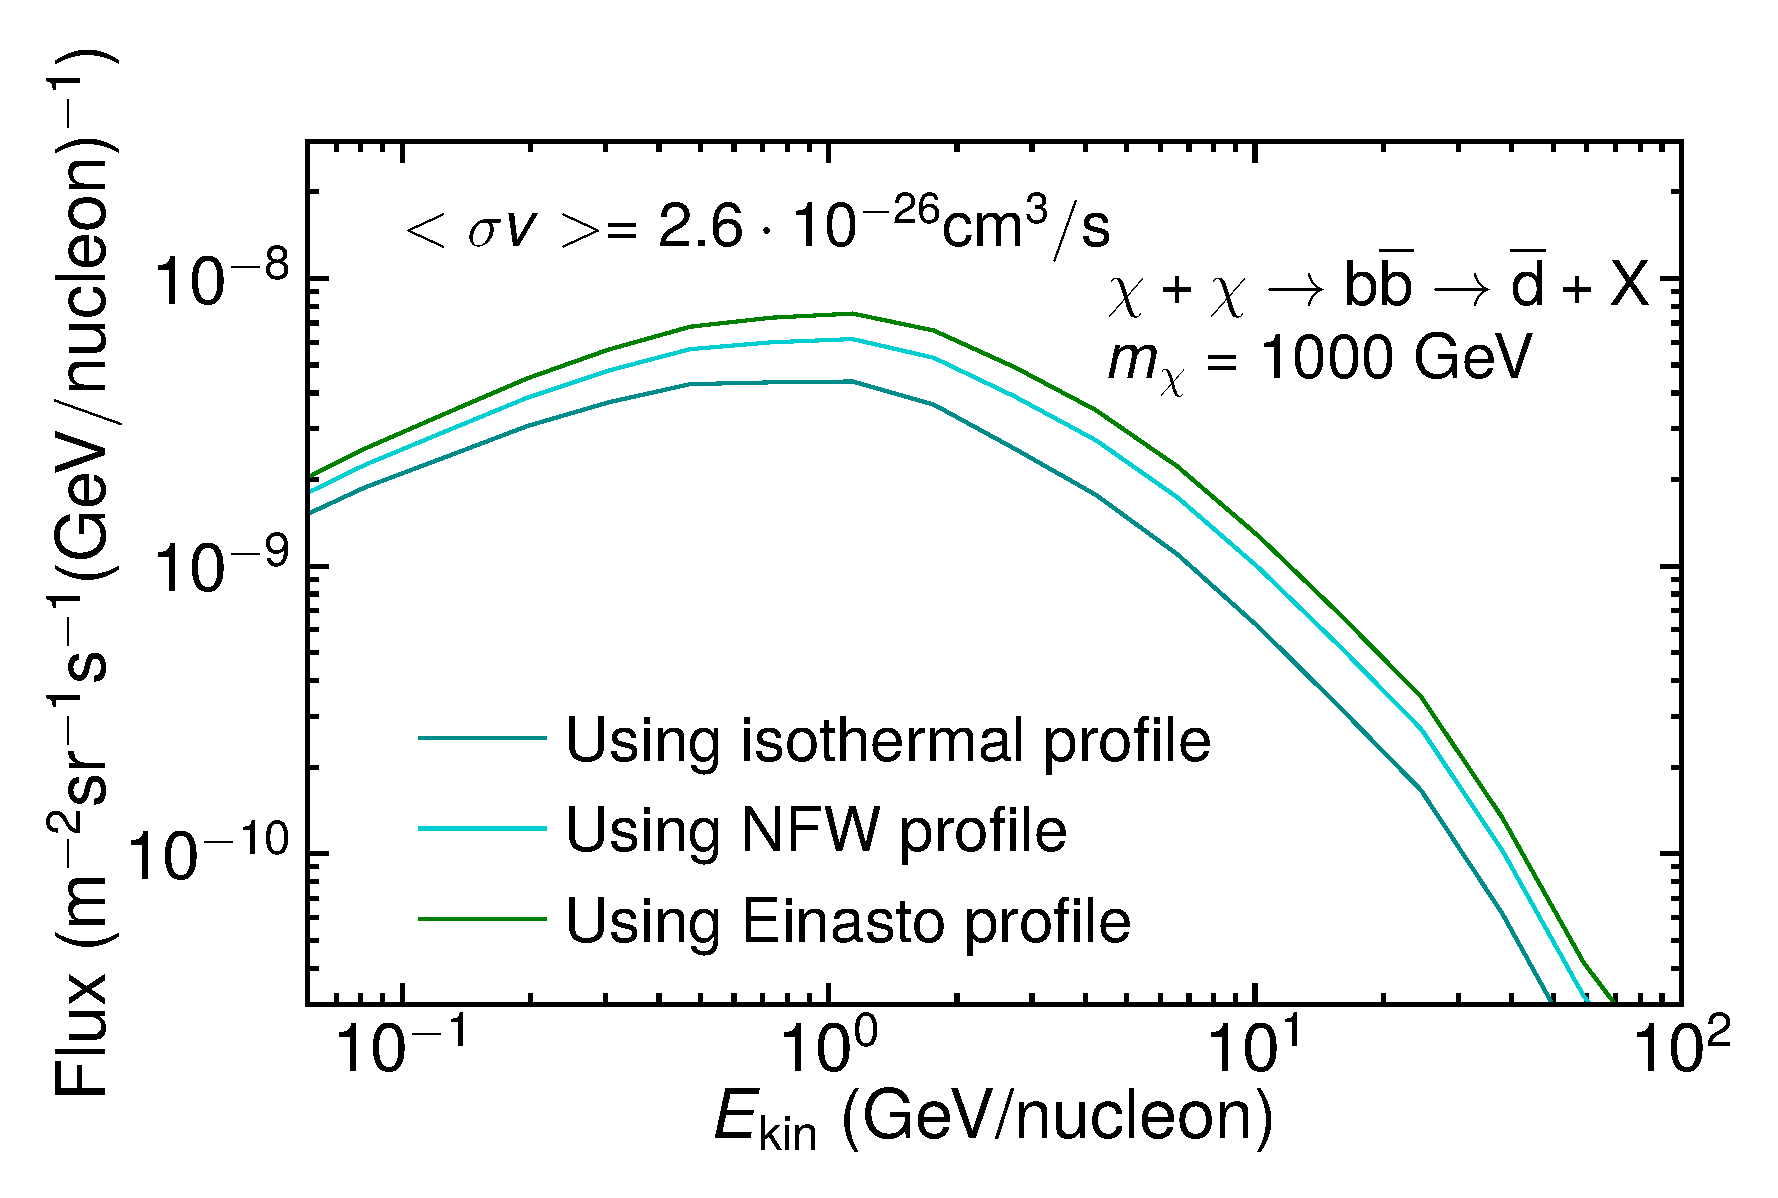
\includegraphics[width=0.48\textwidth]{figures/bbdbarPaperLISDiffProfiles.pdf}
    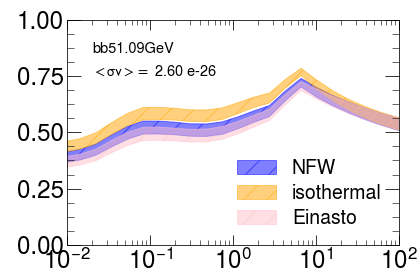
\includegraphics[width=0.48\textwidth]{figures/Transparency_comparison_DM_profiles_bb51GeV_DMXs_option_nominal.png}
    \caption{Antideuteron fluxes for different dark matter profiles (left) and the corresponding transparencies (right), for antideuterons from dark matter annihilation through the \bb\ channel.}
    \label{fig:different_DM_profiles_and_transparencies}
\end{figure}

\subsection{Discussion of the uncertainties on antinuclei fluxes and transparencies}
Presented in this chapter are the experimental uncertainties on the effect of inelastic interactions on antinuclei fluxes in cosmic rays, as well as on the transparency of the galaxy to antinuclei from different sources. It is important to note that these uncertainties are now quantified based on experimental data for the first time, and that they uncertainties are much smaller than other uncertainties in the field, as can be seen by comparing the values given in table \ref{tab:uncertaintiesFluxes}. \\


\begin{table}[htpb]
    \centering
    \begin{tabular}{|c|c|c|c|}
        \hline
        Source of effect & Effect for CR  & Effect for DM & Source \\
        \hline 
        Inelastic interactions $\mathrm{\overline{d}}$ (\ahe\ )& $\pm$20\% (15\%) & $\pm 10 $\% (15\%) & This thesis, \cite{dbar_prop_paper, he3_absorption_paper}\\
        \hline
        Propagation parameters & $\approx$20\% & $\approx$200\% & This thesis, \cite{dbar_prop_paper}\\
        \hline
        Production  $\mathrm{\overline{d}}$ (\ahe\ )& $^{+27}_{-42}$\% ($\pm$ 10-20x) &  $^{+63}_{-70}$\% ($\pm$ 10-30x) & \cite{dbar_prop_paper, Ibarra2014, Korsmeier:2017xzj}\\
        \hline
        DM model uncertainties & N/A & $\approx$ 1000\% & \cite{dbar_prop_paper} \\
        \hline
    \end{tabular}
    \caption{A list of the sizes of uncertainties involved in making predictions for antinuclei fluxes. The second and third column are describing the size of the effect on antinuclei from high energy cosmic ray collisions and from potential dark matter annihilations, respectively.}
    \label{tab:uncertaintiesFluxes}

\end{table}


Another important uncertainty is the model dependence of the transparency, specifically the dark matter mass and annihilation channel dependence. This effect can be seen in the bottom panels of figure \ref{fig:Results_He3_fluxes_diff_DM_masses}. When comparing the transparencies associated with different dark matter mass assumptions for the \WW\ channel, the momentum dependence of the transparency at high energies varies greatly. For higher dark matter masses, the shape of the \ahe\ flux is more similar to the secondary flux than to the flux with the standard \dmm\ assumption of $\approx$100GeV/$c^2$. This results in a transparency which is very similar in both shape and magnitude to the one for secondaries. For the \bb\ channel, the difference in \dmm\ causes a much reduced difference in spectral shape, and the transparencies change shape more slowly with increasing \dmm\ . In particular for the \bb\ channel, a significant difference still remains at low energies, which are the most interesting for indirect dark matter searches. This effect can change the transparencies at high energies from $\approx$50\% for \dmm\ = 100GeV/$c^2$ to almost 90\% at 2 TeV/$c^2$. \\
Another parameter which affects the transparency is the dark matter profile considered. This effect can be seen in figure \ref{fig:different_DM_profiles_and_transparencies}, which shows transparencies for antideuterons from dark matter with different dark matter profiles. It shows that there is an effect depending on the dark matter profile chosen, which can be understood as the mean path length the antinuclei travel before getting to earth. The more peaked Einasto and NFW profiles have lower transparencies, since a larger amount of antinuclei is produced close to the centre of the galaxy (i.e. further away), and this the chance of antinuclei interacting inelastically increases. This effect causes a difference in the transparency between the profiles of about 10\%. 
%Todo
\subsection{Summary of propagation of antinuclei through the galaxy}
From the results in this section several conclusions can be drawn. The most impactful are the novel experimental uncertainties on the effect of the inelastic cross section on antinuclei propagation, i.e. on the transparency. These uncertainites are of the order of 15\% for antihelium, and 10\% for antideuterons, and thus significantly below the uncertainites from other effects, dominantly the uncertainty on the production of these antinuclei. The second conclusion is that the exact shape of the dark matter profile is a minor component in determining the normalization of antinuclei, even before possible degeneracies with antiproton limits are taken into account. This means that even though the dark matter profile is a free choice in current models, the final antinuclei fluxes are not sensitive to this.  The choice of the dark matter mass however has an important effect, both on the shape and the normalization of the resulting antinuclei spectrum. In particular for large WIMP masses, approaching or exceeding masses of 1 TeV, the shape of the spectrum becomes very similar to the shape of the secondary spectrum, which would make differentiation between them difficult. From the considered channels, only the $\Lambda_b$ boosted channel significantly deviated from the others, and only for \ahe\ , which however leaves open the possibility that other not thoroughly considered channels might influence the production of one antinucleus over another. If one were to speculate about the tentative antihelium events seen by the AMS collaboration, which are predominantly at high energies, they might originate from a heavy WIMP, with the \ahe\ production significantly boosted relative to antiproton and antideuteron productions, through some unknown mechanism. What is clear however, is that unraveling the mysteries of such a signal could do wonders for our understanding of antinuclei sources in our galaxy, and might even expose new physics.   



\subsection{Experiments to detect antinuclei in the cosmos}
Given their rarity, antinuclei in cosmic rays are difficult to detect. 

%\subsubsection{Balloon and space bourne experiments}
Detecting antinuclei in cosmic rays has to be done near the top of our atmosphere, since antinuclei would annihilate well before reaching any ground-based detector. This leaves either space bourne experiments or high-altitude balloon flights. Currently there are two promising experiments either currently or soon to be deployed: the Alpha Magnetic Spectrometer (AMS)\cite{} on the international space station (ISS), and the General AntiParticle Spectrometer (GAPS)\cite{}, which is a planned balloon flight experiment. The two are shortly discussed below.\\

The experiment which currently has the best sensitivity for detecting antinuclei is AMS-02, which is a magnetic spectrometer on the international space station. As a magnetic spectrometer, AMS-02 is more sensitive to charge differences, and therefore more sensitive to \ahe\ nuclei than to antideuterons, since the latter need to be distinguished from the significalty more abundant antiprotons. However, it is still a big surprise that AMS has reported potential signals consistent with multiple \ahe\ nuclei, given that none of the currently available models predict a flux within the sensitivity of AMS, much less an order of magnitude above. These reports have cause a large amount of effort from both experimental and theoretical communities to come up with theories which might explain this signal, while also taking into account the lack of evidence for an antideuteron signal. It is currently unclear which process would produce such a large \ahe\ flux without boosting the antideuteron flux in a similar amount, with some suggested options being a boost to \ahe\ production via $\Lambda_b$ decays\cite{}. \\
The current generation of the AMS experiment -- AMS-02 -- has been studying cosmic rays since 2011, having analyzed over 200 billion cosmic-ray events. It consists of several detector systems, including a Time-of-Flight detector, a silicon tracker, a star tracker (to determine its orientation), a transition radiation detector, a permanent magnet to curve charged particle tracks, a Cherenkov detector and an electromagnetic calorimeter. AMS has delivered incredibly precise data on cosmic ray spectra of nuclei up to heavy elements, as well for electrons, positrons and antiprotons. In particular the antiproton spectra have been studies extensively for hints of WIMP dark matter decays, as was already discussed in section \ref{sec:WIMPS}. \\
The "smoking gun" signal which AMS could detect from exotic physics such as dark matter would of course be an antinuclei signal. However, as can be seen from the fluxes in figure \ref{fig:Results_He3_fluxes_diff_DM_masses}, it is not yet clear what source could feasibly reach AMS-02 sensitivities, although several models could do so within all their uncertainties. Therefore it is extremely interesting that AMS has repeatedly reported the observation of multiple possible high-energy \ahe\ and $^4\mathrm{\overline{He}}$ events \cite{}, but as of now these findings have not been published, only presented in talks. The results from one such talk are shown in figure \ref{fig:AMS_MIAPP_talk_ahe}. These events have kinetic energies per nucleon above 10 GeV/c. Should the observed signals indeed be from antihelium nuclei, it comes with a few puzzling questions. Why is the flux so much greater than expected? This increase is possible within uncertainties to be the result of high-energy cosmic-ray collisions, but only under the most favorable conditions. They are also significantly above the expected flux of most dark matter models, however as shown by the study of the $\overline{\Lambda}_b$ boosted \ahe\ flux from dark matter annihilations, some dark matter models could feasibly reproduce these results. One study has concluded that the only standard model process that could plausibly produce such a flux would be an antistar within 1 kpc of earth\cite{}. This would however be very visible from gamma-ray observations, as the large amounts of antimatter--matter annihilations would produce a distinct signal in the gamma-ray spectrum\cite{}. As such, a confirmation of the reported signals would suggest a source beyond the standard model. One possible explanation would be dark matter, where the production of antinuclei is boosted by channels not yet considered. One such example is the recent study on antinuclei production through the $\overline{\Lambda_b}$ channel \cite{}. The second question these findings raise is the scaling of the antinuclei production with each additional nucleon. The number of \ahe\ to $^4\mathrm{\overline{He}}$ events observed suggest a ratio close to 1:3, whereas for production in small systems at the LHC the penalty factor is 1:1000\cite{}. The final question -- and perhaps the easiest to answer -- is why ~10 possible \ahe\ events have been observed while AMS has so far only seen ~7 possible antideuteron events\cite{MIAPP_AMS_talk}. The most likely explanation for this question is simply that differentiating antideuterons from antiprotons is very difficult, as they have the same charge. The background from the antiproton signal might therefore simply cover the sensitivity to an antideuteron flux.\\
\begin{figure}
    \centering
    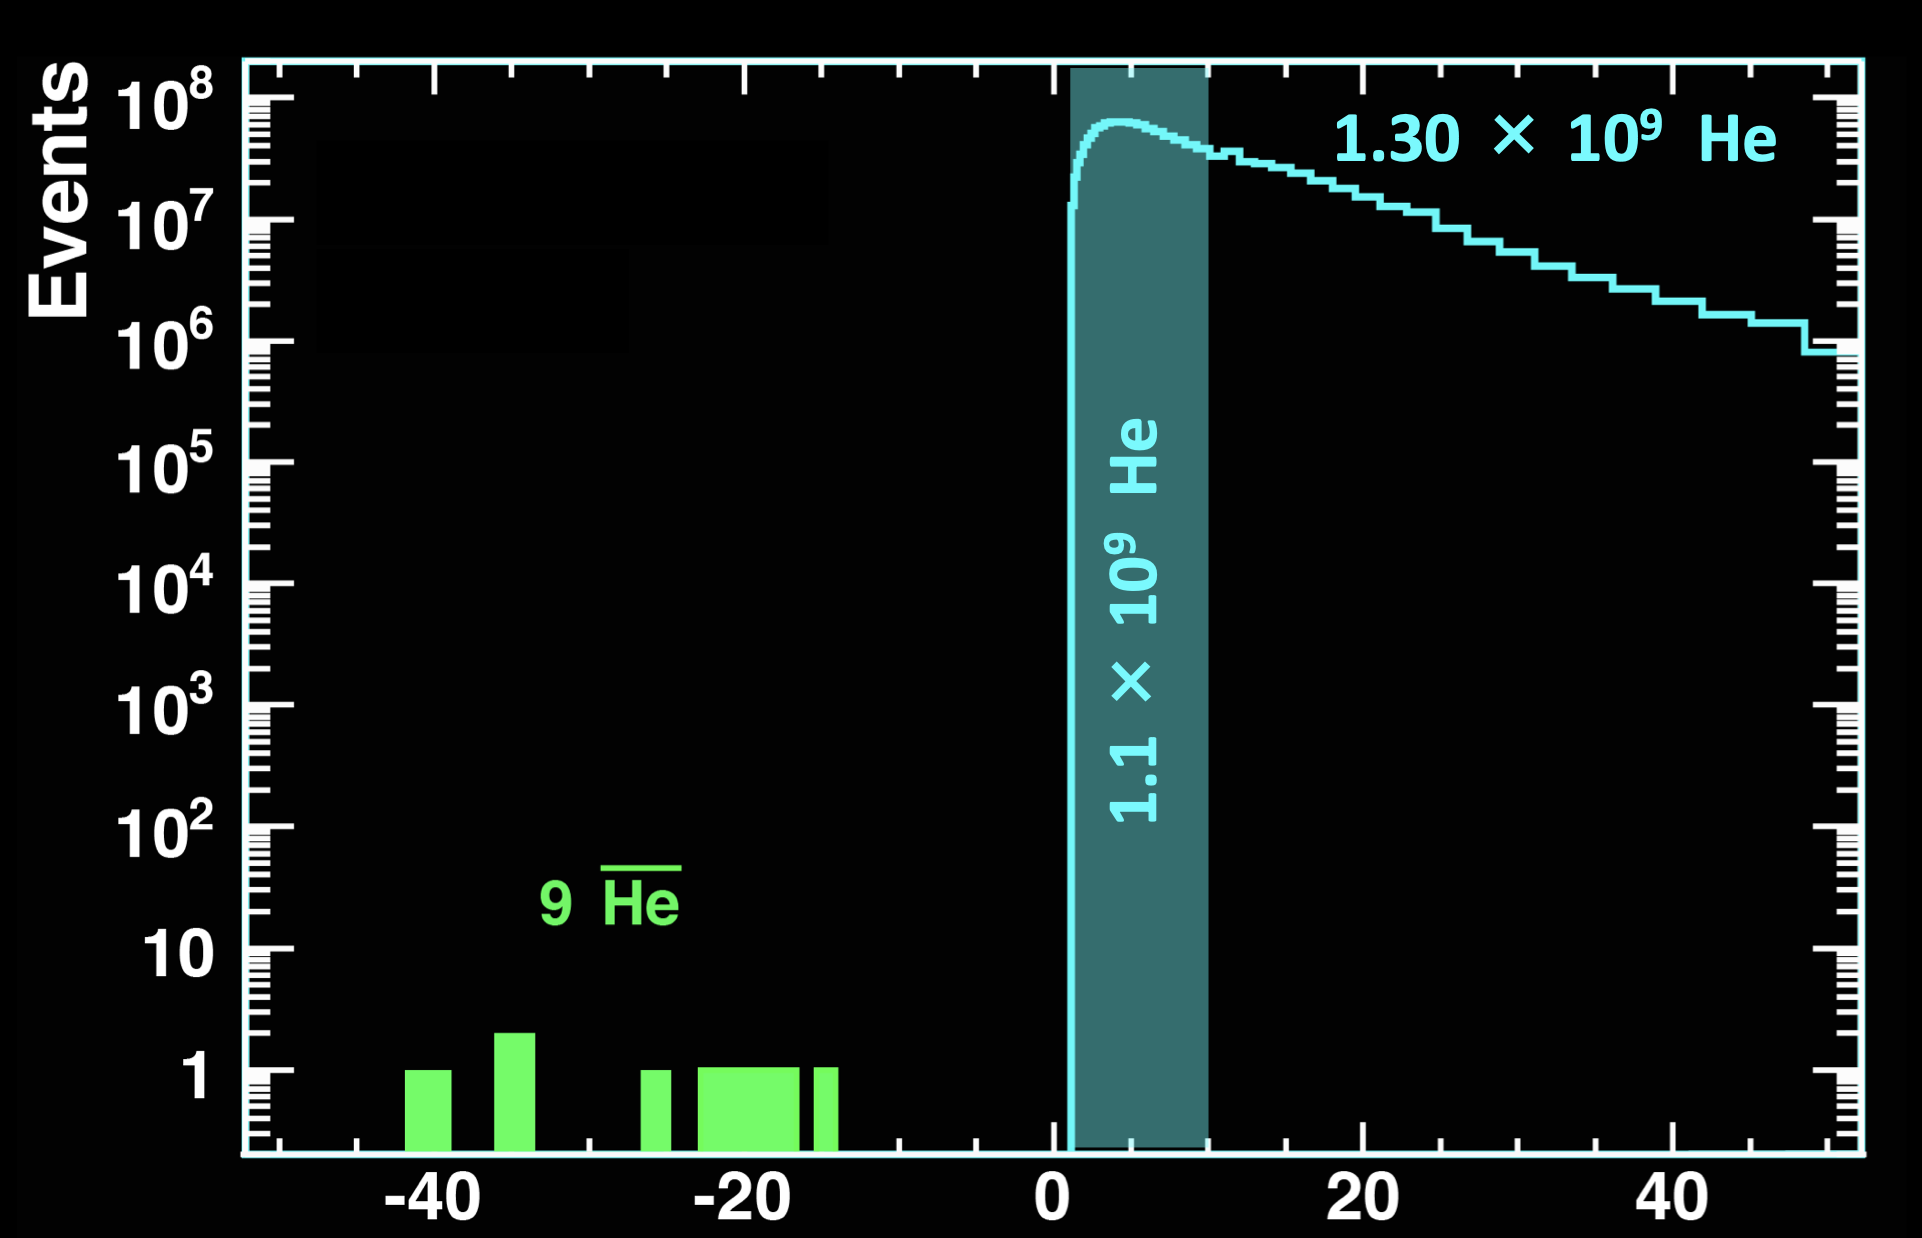
\includegraphics[width=\textwidth]{figures/AMS_he3bar_events_MIAPP.png}
    \caption{Plot of the rigidity resolution of AMS for comparing \ahe\ and $^3\mathrm{He}$ signals. 9 possible \ahe\ events are shown. These findings have not yet been published and this figure is taken from a talk \cite{}.}
    \label{fig:AMS_MIAPP_talk_ahe}
\end{figure}

The current generation of the AMS experiment will hopefully continue to deliver data for years to come - and is even currently being upgraded in order to improve the accuracy of their antiproton measurements - however, planning for the next generation is already ongoing. This next generation experiment is called AMS-100, due to its planned acceptance of 100m$^2$sr \cite{}. It will be a satellite experiment located at Lagrange point 2 of the Sun--Earth system, using many of the same technologies and systems as the James Webb Space Telescope (JWST). AMS-100 would have a 1000 fold increase in acceptance compared to AMS-02, and be able to deal with rigidities up to 100 TV (AMS-02 up to 2 TV). It will also employ a greater magnetic field, using high-temperature superconductors \cite{}. As such, it is expected to deliver more precise measurements of antinuclei in cosmic rays, and thus to shine light on the questions posed by current measurements.\\

GAPS is a more specialised detector, focused less on measuring all kinds of cosmic rays but rather specializing on detecting annihilation events of antimatter. It works based on an outer "umbrella" of TOF detectors around a Si tracker, in order to identify such annihilation events. The setup is shown in figure \ref{fig:GAPS_setup}. A novel technique is used to detect annihilations, called the "exotic atom" technique, which is outlines in figure \ref{fig:GAPS_measurement_technique}. The antiparticle travelling through the detector will loose energy due to Bethe--Bloch ionization until it stops, at which point it will displace an electron in an atom to form an exotic atom with near unit probability. The radiative decay of such an exited atom can be uniquely matched to the components of the exotic atom \cite{}. GAPS will fly over the south pole, where the effects from earth's magnetic field are minimal. The benefit of antinuclei detection via balloon bourne experiments over satellite bourne ones is the much reduced costs.\\

\begin{figure}[hbtp]
    \centering
    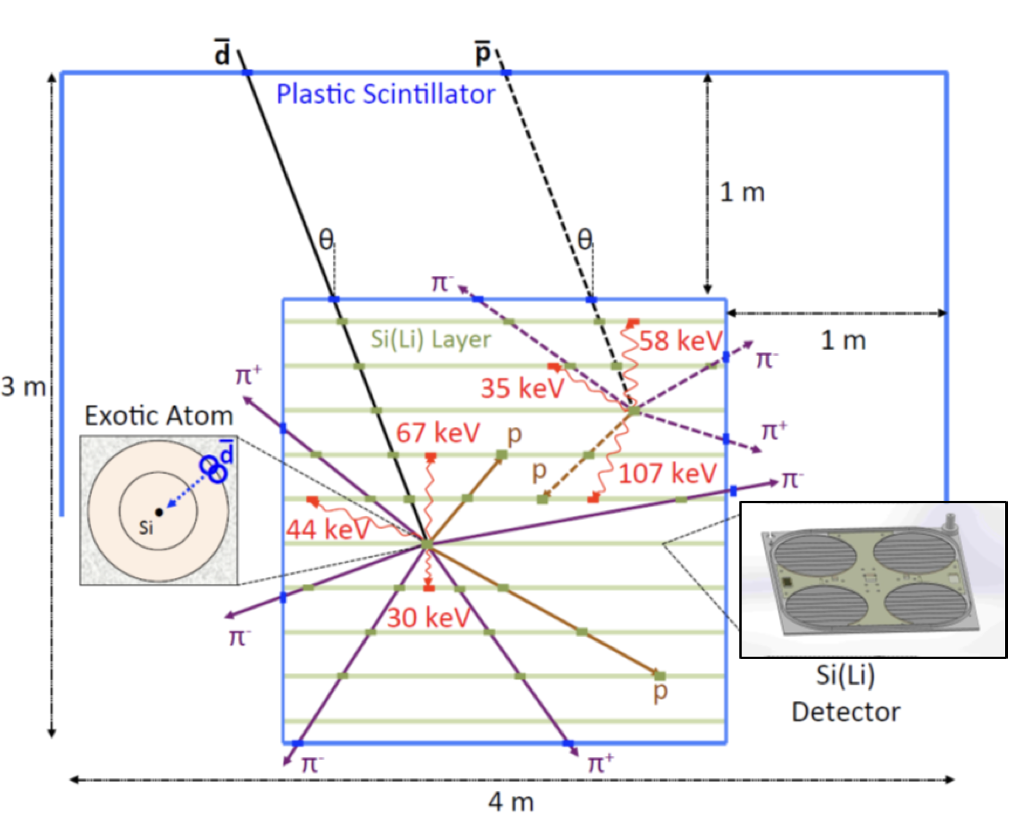
\includegraphics[width=\textwidth]{figures/GAPS_detection_technique.png}
    \caption{GAPS antiparticle detection method: antiparticles slow down and stop in the Si(Li) target, forming an exotic atom. Atomic X-rays will be emitted as it de-excites, followed by the pion (and proton) emission from nuclear annihilation. $\overline{\mathrm{d}}/\overline{\mathrm{p}}$ identification is based on (1) the stopping range, (2) the pion and proton multiplicity, (3) the atomic X-rays energies. Figure and caption taken from \cite{GAPS_method_Vanuccini}.}
    \label{fig:GAPS_measurement_technique}
\end{figure}

\begin{figure}[hbtp]
    \centering
    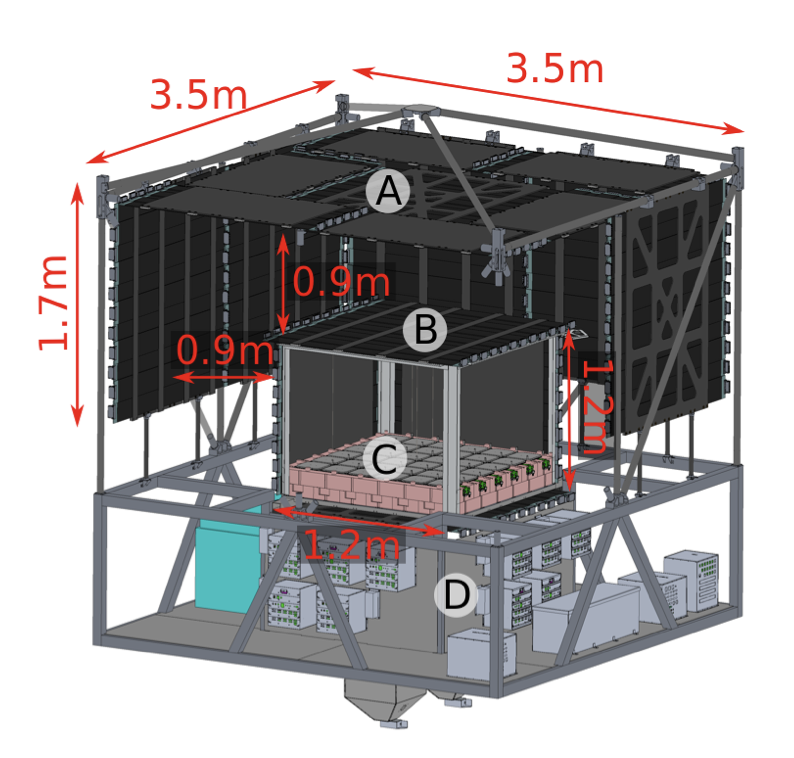
\includegraphics[width=\textwidth]{figures/GAPS_setup.png}
    \caption{The GAPS detector, the central tracker (C) is surrounded by the inner (“cube”, B) and outer (“umbrella”, A) TOF layers. The readout electronics, flight computer, ballast and other support infrastructure are located underneath the tracker (D). Solar panels, cooling systems, antennae and thermal insulation are not shown for clarity. Figure and description taken from \cite{GAPS_setup_Bird}.}
    \label{fig:GAPS_setup}
\end{figure}
The main goal of GAPS is to measure low-energy antideuteron flux, or to improve on the current upper limit, and to follow up on the potential antihelium events seen by the AMS Collaboration. GAPS reach extends to lower energies than those probed by AMS, making such searches complementary. The expected sensitivity to antideuterons of GAPS is shown in figure \ref{fig:Results_dbar_fluxes_diff_DM_masses}, compared with AMS upper limits. As can be seen, the sensitivities are comparable, but GAPS reaches much lower momenta, while AMS covers a much larger momentum span. GAPS is also acting as a pathfinder for future balloon experiments by demonstrating such new technologies, and their usefulness for specific searches. 


%\subsubsection{Developing a cubesat for detecting antiprotons}

